% Options for packages loaded elsewhere
\PassOptionsToPackage{unicode}{hyperref}
\PassOptionsToPackage{hyphens}{url}
\PassOptionsToPackage{dvipsnames,svgnames,x11names}{xcolor}
%
\documentclass[
  12pt,
  a4paperpaper,
]{article}

\usepackage{amsmath,amssymb}
\usepackage{setspace}
\usepackage{iftex}
\ifPDFTeX
  \usepackage[T1]{fontenc}
  \usepackage[utf8]{inputenc}
  \usepackage{textcomp} % provide euro and other symbols
\else % if luatex or xetex
  \usepackage{unicode-math}
  \defaultfontfeatures{Scale=MatchLowercase}
  \defaultfontfeatures[\rmfamily]{Ligatures=TeX,Scale=1}
\fi
\usepackage{lmodern}
\ifPDFTeX\else  
    % xetex/luatex font selection
  \setmainfont[]{Arial}
\fi
% Use upquote if available, for straight quotes in verbatim environments
\IfFileExists{upquote.sty}{\usepackage{upquote}}{}
\IfFileExists{microtype.sty}{% use microtype if available
  \usepackage[]{microtype}
  \UseMicrotypeSet[protrusion]{basicmath} % disable protrusion for tt fonts
}{}
\makeatletter
\@ifundefined{KOMAClassName}{% if non-KOMA class
  \IfFileExists{parskip.sty}{%
    \usepackage{parskip}
  }{% else
    \setlength{\parindent}{0pt}
    \setlength{\parskip}{6pt plus 2pt minus 1pt}}
}{% if KOMA class
  \KOMAoptions{parskip=half}}
\makeatother
\usepackage{xcolor}
\usepackage[top=25mm,left=25mm,right=25mm,bottom=20mm,heightrounded]{geometry}
\setlength{\emergencystretch}{3em} % prevent overfull lines
\setcounter{secnumdepth}{5}
% Make \paragraph and \subparagraph free-standing
\ifx\paragraph\undefined\else
  \let\oldparagraph\paragraph
  \renewcommand{\paragraph}[1]{\oldparagraph{#1}\mbox{}}
\fi
\ifx\subparagraph\undefined\else
  \let\oldsubparagraph\subparagraph
  \renewcommand{\subparagraph}[1]{\oldsubparagraph{#1}\mbox{}}
\fi


\providecommand{\tightlist}{%
  \setlength{\itemsep}{0pt}\setlength{\parskip}{0pt}}\usepackage{longtable,booktabs,array}
\usepackage{calc} % for calculating minipage widths
% Correct order of tables after \paragraph or \subparagraph
\usepackage{etoolbox}
\makeatletter
\patchcmd\longtable{\par}{\if@noskipsec\mbox{}\fi\par}{}{}
\makeatother
% Allow footnotes in longtable head/foot
\IfFileExists{footnotehyper.sty}{\usepackage{footnotehyper}}{\usepackage{footnote}}
\makesavenoteenv{longtable}
\usepackage{graphicx}
\makeatletter
\def\maxwidth{\ifdim\Gin@nat@width>\linewidth\linewidth\else\Gin@nat@width\fi}
\def\maxheight{\ifdim\Gin@nat@height>\textheight\textheight\else\Gin@nat@height\fi}
\makeatother
% Scale images if necessary, so that they will not overflow the page
% margins by default, and it is still possible to overwrite the defaults
% using explicit options in \includegraphics[width, height, ...]{}
\setkeys{Gin}{width=\maxwidth,height=\maxheight,keepaspectratio}
% Set default figure placement to htbp
\makeatletter
\def\fps@figure{htbp}
\makeatother
% definitions for citeproc citations
\NewDocumentCommand\citeproctext{}{}
\NewDocumentCommand\citeproc{mm}{%
  \begingroup\def\citeproctext{#2}\cite{#1}\endgroup}
\makeatletter
 % allow citations to break across lines
 \let\@cite@ofmt\@firstofone
 % avoid brackets around text for \cite:
 \def\@biblabel#1{}
 \def\@cite#1#2{{#1\if@tempswa , #2\fi}}
\makeatother
\newlength{\cslhangindent}
\setlength{\cslhangindent}{1.5em}
\newlength{\csllabelwidth}
\setlength{\csllabelwidth}{3em}
\newenvironment{CSLReferences}[2] % #1 hanging-indent, #2 entry-spacing
 {\begin{list}{}{%
  \setlength{\itemindent}{0pt}
  \setlength{\leftmargin}{0pt}
  \setlength{\parsep}{0pt}
  % turn on hanging indent if param 1 is 1
  \ifodd #1
   \setlength{\leftmargin}{\cslhangindent}
   \setlength{\itemindent}{-1\cslhangindent}
  \fi
  % set entry spacing
  \setlength{\itemsep}{#2\baselineskip}}}
 {\end{list}}
\usepackage{calc}
\newcommand{\CSLBlock}[1]{\hfill\break#1\hfill\break}
\newcommand{\CSLLeftMargin}[1]{\parbox[t]{\csllabelwidth}{\strut#1\strut}}
\newcommand{\CSLRightInline}[1]{\parbox[t]{\linewidth - \csllabelwidth}{\strut#1\strut}}
\newcommand{\CSLIndent}[1]{\hspace{\cslhangindent}#1}

\let\oldsection\section
\usepackage[font=it,labelfont=bf]{caption}
\usepackage{sectsty}
\sectionfont{\centering}
\subsectionfont{\raggedright}
\subsubsectionfont{\raggedright\itshape}
\usepackage{etoolbox}
\AtBeginEnvironment{longtable}{\small}
\pretocmd{\section}{\clearpage}{}{}
\usepackage{romannum}
\makeatletter
\makeatother
\makeatletter
\makeatother
\makeatletter
\@ifpackageloaded{caption}{}{\usepackage{caption}}
\AtBeginDocument{%
\ifdefined\contentsname
  \renewcommand*\contentsname{Table of contents}
\else
  \newcommand\contentsname{Table of contents}
\fi
\ifdefined\listfigurename
  \renewcommand*\listfigurename{List of Figures}
\else
  \newcommand\listfigurename{List of Figures}
\fi
\ifdefined\listtablename
  \renewcommand*\listtablename{List of Tables}
\else
  \newcommand\listtablename{List of Tables}
\fi
\ifdefined\figurename
  \renewcommand*\figurename{Figure}
\else
  \newcommand\figurename{Figure}
\fi
\ifdefined\tablename
  \renewcommand*\tablename{Table}
\else
  \newcommand\tablename{Table}
\fi
}
\@ifpackageloaded{float}{}{\usepackage{float}}
\floatstyle{ruled}
\@ifundefined{c@chapter}{\newfloat{codelisting}{h}{lop}}{\newfloat{codelisting}{h}{lop}[chapter]}
\floatname{codelisting}{Listing}
\newcommand*\listoflistings{\listof{codelisting}{List of Listings}}
\makeatother
\makeatletter
\@ifpackageloaded{caption}{}{\usepackage{caption}}
\@ifpackageloaded{subcaption}{}{\usepackage{subcaption}}
\makeatother
\makeatletter
\makeatother
\ifLuaTeX
\usepackage[bidi=basic]{babel}
\else
\usepackage[bidi=default]{babel}
\fi
\babelprovide[main,import]{english}
\ifPDFTeX
\else
\babelfont{rm}[]{Arial}
\fi
% get rid of language-specific shorthands (see #6817):
\let\LanguageShortHands\languageshorthands
\def\languageshorthands#1{}
\ifLuaTeX
  \usepackage{selnolig}  % disable illegal ligatures
\fi
\IfFileExists{bookmark.sty}{\usepackage{bookmark}}{\usepackage{hyperref}}
\IfFileExists{xurl.sty}{\usepackage{xurl}}{} % add URL line breaks if available
\urlstyle{same} % disable monospaced font for URLs
\hypersetup{
  pdftitle={Socioeconomic Disruption by Artificial Intelligence},
  pdfauthor={Fynn Jonas Rieg},
  pdflang={en},
  colorlinks=true,
  linkcolor={black},
  filecolor={Maroon},
  citecolor={black},
  urlcolor={black},
  pdfcreator={LaTeX via pandoc}}

\title{Socioeconomic Disruption by Artificial Intelligence}
\usepackage{etoolbox}
\makeatletter
\providecommand{\subtitle}[1]{% add subtitle to \maketitle
  \apptocmd{\@title}{\par {\large #1 \par}}{}{}
}
\makeatother
\subtitle{A comparative analysis on labor effects between industries in
the European Union}
\author{Fynn Jonas Rieg}
\date{2023-11-27}

\begin{document}
\maketitle
\setstretch{1.5}
\section*{Abstract}\label{sec-abstract}
\addcontentsline{toc}{section}{Abstract}

Artificial Intelligence technology has seen major breakthroughs in
recent years and is expected to have a significant impact on society.
However, the current literature on the possibly negative effects of AI
on labor is still inconclusive. This paper aims to add to the current
corpus of literature by assessing the relationship between AI innovation
and labor conditions within European industries by looking at European
patent application data and Eurostat's Structural Business Statistics.
The results suggest a decline in the number of employees and their gross
value added for the mining and quarrying industry, positive effects for
labor productivity and gross value added in the information and
communication industry, and mixed effects for the manufacturing
industry, with the number of enterprises and labor costs rising and wage
adjusted labor productivity declining. However, the majority of results
are statistically insignificant. Retrieved data also entail limitations
and need to be interpreted with caution. Consequently, more research is
needed to assess the true relationship between AI innovation and labor
effects.

\newpage{}

\pagenumbering{Roman}

\newpage{}

\setstretch{1}
\renewcommand{\contentsname}{Table of Contents}
\tableofcontents

\newpage{}

\listoffigures

\newpage{}

\listoftables

\newpage{}

\pagenumbering{arabic}
\setstretch{1.5}

\section{Introduction}\label{sec-introduction}

In the last few years, Artificial Intelligence has seen major
breakthroughs in its capabilities and applicable domains
(\citeproc{ref-michael_l_littman_gathering_2021}{Michael L. Littman et
al., 2021, p. 12}). The popular AI chatbot ChatGPT has set a historical
record in its user acquisition pace (\citeproc{ref-hu_chatgpt_2023}{Hu,
2023}), and internet searches for the term ``AI'' are on an all time
high (\citeproc{ref-google_google_2023}{Google, 2023}). This trend has
also arrived in the scientific community, with AI related papers
exploding in popularity in recent years
(\citeproc{ref-catherine_cheung_growth_2022}{Catherine Cheung et al.,
2022}). However, undeniably, the introduction of new technology, this
time, Artificial Intelligence, does raise concerns about its potential
implications on various aspects of society
(\citeproc{ref-gries_artificial_2018}{Gries and Naudé, 2018, p. 1}; see
\citeproc{ref-joint_research_centre_artificial_2018}{Joint Research
Centre, 2018, p. 77}; \citeproc{ref-lu_review_2021}{Lu and Zhou, 2021,
p. 1055}). And even OpenAI's co-founder and chief scientist Ilya
Sutskever admits that ``for every positive application of AGI there will
be a negative as well''\footnote{AGI stands for Artificial General
  Intelligence, which is a form of AI that is capable of performing any
  intellectual task a human can (\citeproc{ref-naude_race_2019}{Naudé,
  2019, p. 4}).} (\citeproc{ref-sutskever_exciting_2023}{Sutskever,
2023}). While AI is not the first technology to raise such concerns
(\citeproc{ref-martens_will_2018}{Martens and Tolan, 2018, p. 5}), the
pace at which AI evolves and advances into various domains is unseen.
Mokyr et al. (\citeproc{ref-mokyr_history_2015}{2015, p. 32}) identifies
two forms of technological anxiety, the fear of labor displacement
through technology and the fear of morally negative applications
resulting in declining welfare. This technological anxiety seems to be
increasing again in recent times, with the majority of the US population
assessing the potential impact of automation as generally unfavorable
rather than beneficial
(\citeproc{ref-anderson_automation_2017}{Anderson, 2017}). Because of
the recent advances in Artificial Intelligence, and its increasing
presence in the media, everyday life, and work, there is a growing need
for research to meticulously scrutinize AI technology's accompanying
concerns to objectively assess its true potential and risks. Given the
seemingly ubiquitous applicability of AI, there is a correspondingly
vast number of possible effects and side effects which AI might induce.
This paper specifically focuses on the aforementioned technological
anxiety of labor displacement. Specifically, Artificial Intelligence's
effects on labor displacement, which in this context also relate to
partial displacements induced by a reduction in labor wages and labor
bargaining power.

The paper is structured as follows: Section~\ref{sec-introduction}
provides an overview about the current literature on automation induces
labor effects. Section~\ref{sec-methodology} introduces the
methodological approach used to assess AI's impact on labor with an
overview of the data sources (Section~\ref{sec-data-sources}), the data
acquisition process (Section~\ref{sec-data-acquisition}) and
preproccessing methods (Section~\ref{sec-preprocessing}), along with the
chosen model (Section~\ref{sec-model}) and its hypotheses
(Section~\ref{sec-hypotheses}). Results are then presented in
Section~\ref{sec-results}, followed by a discussion
(Section~\ref{sec-discussion}) which includes the models' results'
implications (Section~\ref{sec-implications}), important limitations
(Section~\ref{sec-limitations}), and suggestions for future research
(Section~\ref{sec-further-research}). Finally,
Section~\ref{sec-conclusion} concludes the paper and
\nameref{sec-appendix} provides additional tables and figures
accompanying this research.

\subsection{Effects of Artificial Intelligence}\label{sec-effects-of-ai}

Brynjolfsson et al. (\citeproc{ref-brynjolfsson_what_2018}{2018a, p.
46}) found that machine learning affects different types of tasks than
earlier forms of automation. A year later, in a study comparing the
impact of AI on the job market between industries, Webb
(\citeproc{ref-webb_impact_2019}{2019, p. 46}) shows that AI affects
mostly the highly educated workforce and that this group is affected
significantly more by AI than the presence of software or robots. Under
the assumption that the current trend in technological evolution is set
to continue, the speed of labor displacement through technological
innovation is found likely to outpace the speed at which labor can be
relocated (\citeproc{ref-mokyr_history_2015}{Mokyr et al., 2015, p.
43f}.). By constructing impact scores of Artificial Intelligence on
occupations, Felten et al. (\citeproc{ref-felten_effect_2019}{2019})
found low-income occupations to experience a decline in wage growth that
is attributed to the increased presence of AI and middle and high-income
occupations to experience an increase in wage growth (p.~6).
Furthermore, the authors found that occupations with a medium and high
degree of automation (degree of automation being the presence of
automation technologies --- not just AI) positively correlate with
employment when exposed to Artificial Intelligence, while they did not
find any relationship for occupations already exhibiting a low degree of
automation (p.~5). Damioli et al.
(\citeproc{ref-damioli_impact_2021}{2021, p. 14}) linked small and
medium-sized enterprises (SMEs), having previously filed patents related
to AI, to significant increases in labor productivity. The same effect,
however, could not be found once SMEs and large firms were studied
together, nor when only considering large firms (p.14).

It has also been noted that the presence of Artificial Intelligence does
not have a linear impact on labor but depends on influencing factors,
such as price elasticity, complementaries, or elasticity of labor that
govern the implementation of these technologies
(\citeproc{ref-brynjolfsson_what_2017}{Brynjolfsson and Mitchell, 2017,
p. 1533f}.). Additionally, the adoption of AI technology is found to
significantly alter the skill-demand distribution of firms, with the
number of previously highly demanded skills declining while
simultaneously creating demand for new skills
(\citeproc{ref-acemoglu_ai_2020}{Acemoglu et al., 2020a, p. 19}). By
surveying 203 attendees at three AI conferences, Gruetzemacher et al.
(\citeproc{ref-gruetzemacher_forecasting_2020}{2020, pp. 4, 9}) found
attendees, on average, to evaluate 22\% of human tasks being prone to
replacement, with the number rising to 40\% in the next five years.
Researchers have also argued that AI technology can be seen as a new
general purpose technology (GPT) which has implications in every aspect
of society as had other GPTs before, such as the steam engine or
computers (\citeproc{ref-brynjolfsson_artificial_2018}{Brynjolfsson et
al., 2018b, p. 39}). In a meta analysis of the current literature, Lu
and Zhou (\citeproc{ref-lu_review_2021}{2021, p. 1263}) came to the
conclusion that the general consensus among researchers is a definite
concern about AI's implications as well as expected labor displacement,
although unsure about the extent of displacement and whether these
effects are offset elsewhere.

Given the yet small body of empirical literature about the effects of AI
(\citeproc{ref-seamans_ai_2018}{Seamans and Raj, 2018, p. 3}), which is
due to the fact that AI is still a fairly new topic, with real increase
in dominance and interest only seen in recent years
(\citeproc{ref-acemoglu_ai_2020}{Acemoglu et al., 2020a, p. 23f}.), it
is worth noting the effects of previous technologies. The adoption of
machines (specifically often industrial robots
(\citeproc{ref-acemoglu_robots_2020}{Acemoglu and Restrepo, 2020a}; see
\citeproc{ref-graetz_robots_2018}{Graetz and Michaels, 2018})) and
software --- also referred to as computerization
(\citeproc{ref-autor_growth_2013}{Autor and Dorn, 2013};
\citeproc{ref-frey_future_2017}{Frey and Osborne, 2017}; see
\citeproc{ref-pajarinen_computerization_2015}{Pajarinen et al., 2015})
--- have been seen as previous stages in the evolution of automation,
with AI composing the next stage
(\citeproc{ref-acemoglu_harms_2021}{Acemoglu, 2021, p. 19}).
Furthermore, all of these technologies have been summarized under the
umbrella term ``automation'' (\citeproc{ref-mann_benign_2018}{Mann and
Püttmann, 2018, p. 40}) indicating common characteristics and thereby
--- possibly --- common effects.

\subsection{Effects of
Automation}\label{sec-effects-of-automation-on-labor}

In a 2018 study, the introduction of automation technology was found to
have positive effects on employment gains, but only within the same
commuting zone (\citeproc{ref-mann_benign_2018}{Mann and Püttmann, 2018,
p. 26}). These findings contradict the results from Autor et al.
(\citeproc{ref-autor_untangling_2015}{2015, p. 632}), who found no
relation between exposure to automation and employment as a whole but
found a significant decline in employment related to routine tasks in
the non-manufacturing sector (p.~641). Graetz and Michaels
(\citeproc{ref-graetz_robots_2018}{2018, p. 766}) found no relationship
between the usage of industrial robots and net employment. However,
usage of industrial robots was found to lower employment of low-skilled
workers. A later study, also looking at employment effects induced by
usage of industrial robots, found a significant decline of employment as
well as a reduction in wages related to robot exposure within a
commuting zone (\citeproc{ref-acemoglu_robots_2020}{Acemoglu and
Restrepo, 2020a, pp. 2215f, 2218}). Dauth et al.
(\citeproc{ref-dauth_german_2017}{2017, p. 25}) found no relation
between robot exposure and employment in the German market. A few years
later, Dauth et al. (\citeproc{ref-dauth_adjustment_2021}{2021, p.
3126ff}) found robot exposure to lead to within-firm and between-firm
job displacement, with displaced workers having difficulties
reallocating their jobs within the same industry, leading to a migration
of workers from manufacturing (where robot exposure is most present) to
the service sector. They also exhibited that a lack of worker
protections (for example unionization or tenure) is related to greater
displacement. These results were also confirmed by Boustan et al.
(\citeproc{ref-boustan_automation_2022}{2022, pp. 21, 23}) who observed
that displaced workers acquire new skills and concluded job displacement
by automation to be less discernible among unionized and high-skilled
workers. Similarily, Acemoglu and Restrepo
(\citeproc{ref-acemoglu_robots_2020}{2020a, p. 2215f}., 2218) provided
evidence showing automation (adoption of industrial robots) within a
commuting zone (local labor market) relating to significant declines in
employment as well as wages. By studying 53 developing countries, Cirera
and Sabetti (\citeproc{ref-cirera_effects_2019}{2019, p. 172}) did not
find a relationship between exposure to automation and firm level
employment. However, while a net effect on employment was absent, in
line with the aforementioned literature, they did find automation to
alter the composition of tasks and skills within firms (p.~172).

In a purely theoretical approach to the effects of automation on labor,
Acemoglu and Restrepo (\citeproc{ref-acemoglu_low-skill_2018}{2018a, pp.
220, 224}) concluded that automation leads to labor displacement and
that the displacement of low skilled-labor leads to an increase in the
wage gap (pay gap between low-skilled and high-skilled workers) while
the displacement of high-skilled labor is followed by a reduction in the
wage gap as high-skill labor reallocates into medium- and low-skilled
occupations. This reallocation from displaced high-skill labor into
lower skilled occupations has also been shown by Beaudry et al.
(\citeproc{ref-beaudry_great_2016}{2016, p. 21}), who studied the
effects on labor when prices for specific types of labor fall, as is
induced when substitution (through technology) becomes economically
viable. While labor displacement induced by the introduction of
automation is followed by increased inequality between low-skill and
high-skilled labor in the short run
(\citeproc{ref-acemoglu_race_2018}{Acemoglu and Restrepo, 2018b, p.
1519}), the creation of new tasks --- that is followed by increased
productivity gains from automation --- is seen to reduce this gap in the
long run (p.~1521). However, this positive outlook of a net positive on
employment only holds true as long as the productivity effects, which
accompany the adoption of automation technologies, offset the
displacement effects incurred in the first place. And should the offset
be insufficient, automation is found to negatively impact the demand for
labor and its wages (\citeproc{ref-acemoglu_artificial_2018}{Acemoglu
and Restrepo, 2018c, p. 227}). There is also growing evidence suggesting
automation to cause a decline in real wages of low-skilled workers, for
example, Acemoglu and Restrepo
(\citeproc{ref-acemoglu_unpacking_2020}{2020b, p. 360f}.) found strong
relationships between the adoption of automation technology and wages.
Acemoglu and Restrepo (\citeproc{ref-acemoglu_tasks_2022}{2022, p.
1993}) found a relationship between labor displacement and a decrease in
relative wages, concluding automation to cause an increase in wage
inequality (p.~1998). Automation is also attributed to the decline in
the demand for labor in the US over recent decades
(\citeproc{ref-acemoglu_automation_2019}{Acemoglu and Restrepo, 2019, p.
21}).

Furthermore, Arntz et al. (\citeproc{ref-arntz_risk_2016}{2016, p. 14f})
studying 21 OECD countries found 9\% in the US, and 6-12\% across
countries of overall employment to be substitutable for automation,
while Acemoglu and Autor (\citeproc{ref-acemoglu_skills_2011}{2011, p.
61}) came to the conclusion that labor displacement by machines mostly
affects routine tasks.

\subsection{Effects of
Computerization}\label{sec-effects-of-computerization}

In a Finnish study, Pajarinen et al.
(\citeproc{ref-pajarinen_computerization_2015}{2015}) came to the
conclusion that computerization is likely to place high risk of
displacement on 35\% of the Finnish labor market (p.~5), 33\% of
Norwegian labor (p.~5) as well as 49\% in the US (p.~5). Frey and
Osborne (\citeproc{ref-frey_future_2017}{2017, p. 41}) found 47\% of US
employment to have a a high risk suitability for substitution by
computerization. They further classify the process of automation into
two ``waves'' with the first wave affecting routine tasks
(transportation, logistics, office and administration) (p.~41) followed
by a second wave that, once technological obstacles are overcome, will
affect the jobs involving creative or abstract tasks (p.~43). Evidence
also suggests computerization to significantly induce labor displacement
from occupations relying on routine tasks into higher-skilled
occupations as well as low-skilled service occupations
(\citeproc{ref-autor_growth_2013}{Autor and Dorn, 2013, p. 1573})

\subsection{Changes in Occupational
Composition}\label{sec-changes-of-occupational-composition}

Furthermore, it is important to note that previous research on the
effects of robots, software and AI --- that have been summarized under
the umbrella term ``automation'' (\citeproc{ref-mann_benign_2018}{Mann
and Püttmann, 2018, p. 40}) --- in general may not have found net
negative effects on employment but a restructuring of composition of
occupations. The aforementioned study from Autor et al.
(\citeproc{ref-autor_untangling_2015}{2015, p. 644}) found automation,
while having no aggregate effects on employment, led to a decline in
occupations involving routine tasks and an increase in non-routine
(abstract) tasks. Graetz and Michaels
(\citeproc{ref-graetz_robots_2018}{2018, p. 766}) found the same effect
studying the introduction of industrial robots. Furthermore, using
weighted patents and firm level data together with Eurostat's Structural
Business Statistics, Van Roy et al.
(\citeproc{ref-van_roy_technology_2018}{2018, p. 7}) reasoned
technological innovation to only have positive effects on employment on
firm level as well as in high-tech and medium-tech sectors, and found no
relationship between technology innovation and employment in the service
sector. These effects remain only harmless as long as the assumption
holds true that displaced labor can in fact always reallocate itself to
new tasks. Should this assumption be contradicted, and the negative
effects of automation on employment are no longer offset by the positive
effects of reallocation, the phenomenon of occupational migration would
turn into an observation of job destruction.

\subsection{Changes in Labor Share}\label{changes-in-labor-share}

The introduction of capital, whether to complement or substitute labor,
inehrently leads to a decline of a firm's profits paid to labor as the
share of labors input relative to the output value decreases (assuming
all else equal). And in fact Karabarbounis and Neiman
(\citeproc{ref-karabarbounis_global_2014}{2014, p. 99}) show that the
observed decline in capital prices explains almost half the decline in
global labor share that has been observed in recent decades. This might
seem problematic as an increasing portion of a firm's revenue remains as
corporate profits and savings (given that the capital invested leads to
a decrease in marginal costs through substitution of labor and/ or
increased production) rather than being redistributed to labor.
Karabarbounis and Neiman (\citeproc{ref-karabarbounis_global_2014}{2014,
p. 102}) further show that the observed decline in labor share is
accompanied by an increase in corporate revenue and savings. This is
also brought forward from Acemoglu and Restrepo
(\citeproc{ref-acemoglu_automation_2019}{2019, p. 27}) who conclude that
``{[}\ldots{]} automation always reduces the labor share and may reduce
labor demand {[}\ldots{]}'' but also mention that the creation of new
tasks necessarily increases the labor share. These results where further
solidified by Acemoglu et al.
(\citeproc{ref-acemoglu_competing_2020}{2020b, p. 387}) who investigated
the French manufacturing market and found firms exposed to automation
(in this study measured by the introduction of robots) to experience
significant declines in their labor share.

\subsection{Definitions of AI}\label{sec-definitions-of-ai}

Lastly, research on Artificial Intelligence's implication has been
intrinsically difficult due to the fact that there is no consensus in
the definition of AI yet (\citeproc{ref-damioli_impact_2021}{Damioli et
al., 2021, p. 7}; see \citeproc{ref-lu_review_2021}{Lu and Zhou, 2021,
p. 1063}). The classification of Artificial Intelligence remains also
difficult due to the fact that there is yet no widespread agreement on
the definition of intelligence itself (see
\citeproc{ref-legg_collection_2007}{Legg and Hutter, 2007}). While AI
and machine learning are sometimes regarded as two different terms, the
former applying to the industry and the latter applying to the
technology (\citeproc{ref-crawford_atlas_2021}{Crawford, 2021, p. 9}),
in this research, the term Artificial Intelligence refers to the
underlying technologies and its applications.

\subsection{Summary}\label{sec-summary-of-effects}

To conclude, the net impact assessment of automation on socioeconomic
factors widely differs in the aforementioned literature (see also
\citeproc{ref-frank_toward_2019}{Frank et al., 2019, p. 6532}). Some
research has focused on mircoeconomic data (see
\citeproc{ref-seamans_ai_2018}{Seamans and Raj, 2018}) or local labor
markets (commuting zones) (see
\citeproc{ref-acemoglu_robots_2020}{Acemoglu and Restrepo, 2020a};
\citeproc{ref-autor_untangling_2015}{Autor et al., 2015};
\citeproc{ref-autor_growth_2013}{Autor and Dorn, 2013}), while other
research has focused on national effects (see
\citeproc{ref-furman_ai_2019}{Furman and Seamans, 2019}) and
international effects (see \citeproc{ref-graetz_robots_2018}{Graetz and
Michaels, 2018}). While one would expect to see the same relationship
between the chosen variables on all levels, apart from differences in
research design, it may be difficult to assess effects on a greater
aggregate level as the number of variables that would need to be
included to account for differences between and within groups becomes
unfeasible. Given the various contradicting results on the relationship
between automation and labor effects and the increasing presence of AI,
this research aims to add to the current corpus of literature by
assessing the relationship between AI innovation and socioeconomic
factors. Specifically, the research question is as follows: How does AI
innovation across industries impact labor displacement and labor
conditions?

\section{Methodology}\label{sec-methodology}

The following section introduces the methodology adopted in this
research along with the data sources used, the data acquisition process,
the data preprocessing methods as well as an overfiew of the data, the
chosen model and its hypotheses. Note that the data acquisition,
preprocessing, as well as the statistical models, figures and tables
presented in this research have been implemented in Python and are
available in the GitHub repository accompanying this research
(\citeproc{ref-rieg_bt_ai_2023}{Rieg, 2023}). The repository also
contains the source code for this paper as a Quarto
(\citeproc{ref-allaire_quarto_2022}{Allaire et al., 2022}) document as
well as seperate source code for most tables and figures provided in
this paper. To keep domain specific technicalities about the
implimentation of the following methdology to a minimum, methods are
mostly described in their characteristics and not in their
implementation. While the GitHub repository contains the source code,
for attribution purposes, it should be noted that the data acquisition
process via EPO'S API was implemented using Python's Requests module
(\citeproc{ref-chandra_python_2015}{Chandra and Varanasi, 2015}),
processing and table creation was done using Pandas
(\citeproc{ref-the_pandas_development_team_pandas-devpandas_2023}{The
pandas development team, 2023}), Numpy
(\citeproc{ref-harris_array_2020}{Harris et al., 2020}) and SciPy
(\citeproc{ref-virtanen_scipy_2020}{Virtanen et al., 2020}). Regressions
and statistical tests were implemented with the Statsmodels module
(\citeproc{ref-seabold_statsmodels_2010}{Seabold and Perktold, 2010})
and figures were created using Plotly
(\citeproc{ref-plotly_technologies_inc_collaborative_2015}{Plotly
Technologies Inc, 2015}).

A key problem to current AI research is the lacking availability of
precise data about the usage and implementation of AI technologies
(\citeproc{ref-seamans_ai_2018}{Seamans and Raj, 2018, p. 5f}.).
Therefore, this research adopts an approach which has similarities to
Mann and Püttmann (\citeproc{ref-mann_benign_2018}{2018, p. 13}) who
used patent counts as a proxy for estimating the level of automation
present within a US commuting zone and Van Roy et al.
(\citeproc{ref-van_roy_technology_2018}{2018}) who used firm-level
citation-weighted patent counts to measure effects on employment.
However, the here presented method of patent selection differs. While
Mann and Püttmann (\citeproc{ref-mann_benign_2018}{2018}) classified
texts based on the tasks they may effect within occupations, the
presented approach here uses API query composition to preselect patents
whose titles or abstracts match keywords reserved to an industry. It
should be noted that there have been other approaches to measure the
presence of AI, such as using the AI Progress Measurement from the
Electronic Frontier Foundation (EFF), job postings
(\citeproc{ref-acemoglu_ai_2020}{Acemoglu et al., 2020a, p. 12}) and
surveys (\citeproc{ref-gruetzemacher_forecasting_2020}{Gruetzemacher et
al., 2020, p. 4}). However, the EFF project, while being a promising
source of data, has been discontinued in 2017
(\citeproc{ref-electronic_frontier_foundation_ai_2017}{Electronic
Frontier Foundation, 2017}).

\subsection{Data Sources}\label{sec-data-sources}

Data about patent publications is obtained from the European Patent
Office's Open Patent Services (OPS) API
(\citeproc{ref-european_patent_office_open_2023}{European Patent Office,
2023}) as well as the Annual Structural Business Statistics (SBS) by
Eurostat
(\citeproc{ref-european_commission_eurostat_structural_nodate}{European
Commission, Eurostat, n.d.a}). Furthermore, Eurostat's code lists of
Statistical classification of economic activities in the European
Community (NACE Revision 2)
(\citeproc{ref-european_commission_eurostat_statistical_2023}{European
Commission, Eurostat, 2023a}) (henceforth ``NACE'') and economic
indicators for Eurostat's SBS
(\citeproc{ref-european_commission_eurostat_economical_2023}{European
Commission, Eurostat, 2023b}) are retrieved to map codes to their
respective definition. Additionally Cooperative Patent Classification
(CPC) codes are retrieved manually from the European Patent Office's
Espacenet website
(\citeproc{ref-european_patent_office_classification_nodate}{European
Patent Office, n.d.a}).

\subsubsection{Patents}\label{patents}

Cooperative Patent Classification is a classification system by the
European Patent Office and the US Patent and Trademark Office that
allows for a structural hierarchical classification of patents
(\citeproc{ref-european_patent_office_cooperative_nodate}{European
Patent Office, n.d.b}). As seen in Table~\ref{tbl-cpc-codes}, CPC codes
are composed of a section (alphabetical), class (numerical), subclass
(alphabetical), and main group (numerical). The CPC codes are used to
retrieve patents that utilize artificial intelligence technology. The
European Patent Office's OPS API allows for programmatic access to the
Patent Office's database
(\citeproc{ref-european_patent_office_open_2023}{European Patent Office,
2023}). With it, one can retrieve data on individual patents, such as
--- among others --- their title and abstract, date of application,
place of application, the names of the applicants, the patents
classification (CPC), and a patent's references to other patents and
documents. The OPS is used to systematically retrieve patents that
contain specified attributes (see Section~\ref{sec-data-acquisition}).
Retrieved patents are used as a proxy for the current level of interest
and level of innovation in AI, which in turn is assumed to be an
indicator for the extent to which AI is present within an industry.

\subsubsection{Structural Business
Statistics}\label{structural-business-statistics}

Eurostat's Structural Business Statistics (SBS) are annually composed
statistics about the economic structure and performance of businesses
across the EU as well as aggregates on EU level. It currently holds data
for the years 2005 to 2020
(\citeproc{ref-european_commission_eurostat_structural_nodate-1}{European
Commission, Eurostat, n.d.b}).\footnote{At the time of writing, the
  Eurostat has released its latest data on the SBS for the year 2021
  (\citeproc{ref-eurostat_enterprises_2023}{Eurostat, 2023a}).
  Unfortunately, the new statistics uses new indicators that do not
  align with previous ones
  (\citeproc{ref-european_commission_commission_2020}{European
  Commission, 2020, p. 131}).} It gathers data from national sources and
calculates EU wide aggregates on the level of NACE sections and groups
about a variety of indicators, such as the number of enterprises present
in an industry, the number of employees, and monetary value produced
(\citeproc{ref-european_commission_commission_2009}{European Commission,
2009}). While the SBS offers a variety of indicators (see
\citeproc{ref-european_commission_commission_2009}{European Commission,
2009}), this research focuses on the following. First, the number of
enterprises present within an industry. This variable has been chosen to
describe a possible relationship between the current number of AI patent
applications and a possible trend towards a monopolistic market
structure. The intuition here being that a market trending towards
monopoly (not actually exhibiting monopoly) gains increasing leverage
(bargaining power) over labor.

Second, the number of Employees. Given the literature introduced in the
previous section, one would expect two possible relationships between
the number of patents retrieved and the number of employees. Either
technology acts as a complementary input, enhancing labor productivity
and leading to industry growth, which further induces demand in labor.
Here one would expect to see a positive relationship between the
endogenous and exogenous variables. Or technology acts as a substitute
for labor, i.e., displacing labor at a rate higher than new occupations
are introduced into the industry. In this case, one expects a negative
relationship between the introduction of technology and the number of
employees.

Third, the wage adjusted labor productivity. It is expressed as a ration
of value added over average personnel expenses
(\citeproc{ref-european_commission_eurostat_wage_2023}{European
Commission, Eurostat, 2023c}). This variable has been chosen to describe
a possible relationship between the current number of AI patent
applications and the productivity of labor. Given the two possibilities
that new technology either displaces labor completely or complements
labor (which may include some displacement that is fully offset by the
creation of new jobs), the expectation is that the introduction of
technology always enhances labor productivity (either through
displacement or complementation). Both ways should exhibit a rise in
wage adjusted labor productivity as the numerator of the ratio
increases. Of course, there may be scenarios in which simultaneously the
denominator --- wages --- increases too.

Fourth, gross value added per employee. This variable was chosen on the
assumption of increased productivity through the adoption of new
technology. As capital (in this case AI technology) aids to increase
output production on a marginal (per employee) basis, one would expect
the ratio to grow with increased adoption of technology.

Fifth, the percentage of personnel costs in production, which is a
derived value from production costs and personnel costs, calculated by
Eurostat
(\citeproc{ref-european_commission_eurostat_derived_nodate}{European
Commission, Eurostat, n.d.c, p. 1}). One would expect --- all else equal
--- the percentage share of labor costs in the production process to
decrease with the adoption through technology. Either because capital
spending is increased, or marginal costs of capital is decreased, or
production quantity (and value ) is increased by adoption of new
technology. The SBS data's indicators are used as the endogenous
variables to be explained by the number of retrieved patent
applications.

\subsubsection{Definition of AI}\label{definition-of-ai}

To retrieve patents that relate or incorporate to AI technology, the
selection of correct CPC codes is crucial. While there are a variety of
possible technologies that may fall under the umbrella term ``Artificial
Intelligence'', this research aims to assess AI's socioeconomic impact,
which, if negative, falls into the governmental realm. Therefore, a
legal definition of AI is preferable as a classifier on which basis CPC
codes are selected. Furthermore, it is arguable that the political
definition is likely to have the greatest (socio)economic impact in the
near future due to possible (and probable) regulation. However, as there
is no legal definition yet --- at least in the EU --- technologies
listed in the European Commision's latest proposal for the ``Artificial
Intelligence Act{[}'s{]}''
(\citeproc{ref-european_commission_proposal_2021}{European Commission,
2021a}) annex (\citeproc{ref-european_commission_annexes_2021}{European
Commission, 2021b}) will be used.\footnote{The European Commission's
  proposal for the ``Artificial Intelligence Act'' is currently in the
  legislative process. At the time of writing, the European Parliament
  has made amendments to this proposal, one of which --- unfortunately
  --- is the removal of the list of technologies classified as AI from
  the initial proposal's annex
  (\citeproc{ref-european_parliament_texts_2023}{European Parliament,
  2023, p. 326f}.). For the time being, the EU Parliament's new
  definition (amendment 165, p.~111f.) of Artificial Intelligence is
  rather vague, which is why the European Comission's initial proposal's
  definition will be used.} In its annex \Romannum{1}, the European
Commsission suggests the following definition for AI.

\setstretch{1}

\begin{quote}
``(a) Machine learning approaches, including supervised, unsupervised
and reinforcement learning, using a wide variety of methods including
deep learning;\\
(b) Logic- and knowledge-based approaches, including knowledge
representation, inductive (logic) programming, knowledge bases,
inference and deductive engines, (symbolic) reasoning and expert
systems;\\
(c) Statistical approaches, Bayesian estimation, search and optimization
methods.'' (\citeproc{ref-european_commission_annexes_2021}{European
Commission, 2021b, p. 2})
\end{quote}

\setstretch{1.5}

As there is no clear mapping between the European Commission's
definition and available Cooperative Patent Classification codes, CPC
codes are chosen to the author's best knowledge.

\setstretch{1}

\phantomsection\label{tbl-cpc-codes}
\begin{longtable}[]{@{}ll@{}}
\caption{\label{tbl-cpc-codes}Selected CPC Codes}\tabularnewline
\toprule\noalign{}
Class & CPC \\
\midrule\noalign{}
\endfirsthead
\toprule\noalign{}
Class & CPC \\
\midrule\noalign{}
\endhead
\bottomrule\noalign{}
\endlastfoot
Machine Learning & G06N20/00, G06N20/10, G06N20/20 \\
Supervised Learning & G06N3/09 \\
Unsupervised Learning & G06N3/088 \\
Reinforcement Learning & G06N3/092 \\
Deep Learning & G06N3/08 \\
\end{longtable}

\setstretch{1.5}

\subsection{Data Acquisition}\label{sec-data-acquisition}

In order to retrieve data from the European Patent Office's Open Patent
Services (OPS) API, queries are composed to link retrieved patents to
their respective industry. The query composition is based on the
selected CPC codes displayed in Table~\ref{tbl-cpc-codes}, as well as
keywords from the list of NACE codes that have been retrieved from
Eurostat. Each NACE code is composed of section (alphabetical), division
(numerical), group (numerical) and class (numerical) of a particular
economic activity. Sections relate to the overall industry, while
divisions, groups and classes relate to more specific activities within
the industry (\citeproc{ref-eurostat_nace_2023}{Eurostat, 2023b}). For
each industry, keywords are extracted from the NACE code's description.
This is done on the division level (the second level of NACE codes). As
a result, keywords are extracted and grouped by their respective
division. For example, for NACE industry ``A'', which relates to
``agriculture, forestry and fishing''
(\citeproc{ref-european_commission_eurostat_economical_2023}{European
Commission, Eurostat, 2023b}), keywords are extracted for its three
divisions, ``crop and animal production, hunting and related service
activities'' (A01), ``forestry and logging'' (A02), and ``fishing and
aquaculture'' (A03). To ensure only relevant keywords are used, each
description is cleaned of common characters and unrelated words (e.g.,
``,'', ``and'', ``or'', ``to'') as well as duplicate words. Descriptions
for each industry are then split into lists of single keywords that will
be used in the API query. As a result, extracted keywords are
identifiable by their section as well as division.

Because some industries contain a variety of different activities (e.g.,
NACE industry (section) ``A'' relates to ``Agriculture, forestry and
fishing''
(\citeproc{ref-european_commission_eurostat_economical_2023}{European
Commission, Eurostat, 2023b})), main (industry) keywords that relate to
the section as a whole are manually selected (see
Table~\ref{tbl-nacemainkeywords} in the \nameref{sec-appendix}). In
other words, while general (division) keywords are selected from the
descriptions of groups within a division, main keywords are extracted
from the description of a section. For each division within a section
(industry), queries are then build using the (manually selected) main
(industry) keywords, the general (division) keywords, as well as the
chosen CPC codes. The general structure of a query is as follows.
Queries are build on the level of divisions. For each division, a query
is composed that retrieves patents that have at least one of the main
keywords of the respective section (industry) in its title or abstract,
at least one keyword of the division's general keywords in its title or
abstract, at least one of the chosen CPC codes in the patent's list of
CPC codes, and an application number starting with ``EP'', relating to
the European Patent Office.\footnote{To be precise, because of the API's
  restrictions, there can be multiple queries for the same division. The
  OPS API allows for a maximum number of 20 ``terms'' (keywords, such as
  a single CPC code or industry keyword) but also only a maximum number
  of 10 terms per argument (such as keywords that must be contained in
  the patent's title or abstract; the argument is ``title or
  abstract''). Given that each query contains seven CPC codes and one
  application number, if there are together more than 12 main keywords
  and general keywords, the general keywords are subdivided into smaller
  chunks across multiple queries. Therefore, each query contains all
  main keywords, CPC codes and the application number, while the
  remaining terms are filled with the general keywords.}

The resulting query is then used to retrieve patents from the OPS API.
Initially, queries were created not only for the European Patent Office
but all patent offices within the European Union to retrieve patent data
on a national level. This approach would have resulted in a much richer
dataset and enabled better aggregates while also allowing for
between-country comparisons. However, initial tests showed that most of
the patents filed with a national patent office contain only patent
titles and abstracts in their native language which renders the chosen
keywords in the query language (English) ineffective. As a result, the
decision was made to only retrieve patents filed with the European
Patent Office. This approach disregards patents filed with national
patent offices. The query is composed of the following elements:

\setstretch{1.0}

\begin{quote}
\textbf{(ta = Main Keywords) AND (ta = Description Keywords) AND (cpc =
CPC Codes) AND (ap = ``EP'')}\\
\emph{Note: ta = title or abstract; ap = Application Number, referring
to the Patent Office the patent was filed at. In this case, ``EP''
refers to the European Patent Office. See Table~\ref{tbl-queryexample}
for example queries.}
\end{quote}

\setstretch{1.5}

The queries are then posted to the OPS API's Published Data Keywords
Search with Variable Constituents endpoint
(\citeproc{ref-european_patent_office_published_nodate}{European Patent
Office, n.d.c}). The API's response, containing the data --- which is
provided in JSON format --- is first enriched with meta data, such as
the section and division for which the query was posted, to allow a
mapping from the returned patents to the industry to which they belong.
Next, the data is converted from JSON format into a table (Pandas
DataFrame). Given the structure of JSON files, this is not a linear
process. Therefore, only relevant information, such as the patent office
of application, the industry (section) and division, the CPC codes, the
patents filing dates, names of inventors, and citation, have been
extracted from the JSON file. The resulting table contains individual
patents and their attributes together with the meta data of the query's
section and division through which each patent has been retrieved.

\subsection{Preprocessing}\label{sec-preprocessing}

Since Eurostat's SBS data only includes codes to refer to given
indicators as well as industries, data retrieved from Eurostat (SBS, and
Code Lists about NACE and SBS codes) is merged. This is done by matching
the NACE codes and SBS indicator codes to the respective NACE code and
indicator in the SBS data. The economic indicators ``Enterprises'' and
``Persons employed'' are reported as totals. ``Wage adjusted labor
productivity (Apparent labor productivity by average personnel costs)''
and ``Share of personnel costs in production'' are reported as
percentages, and ``Gross value added per employee'' is reported in
Euros. Because the number of employees is rather large for each
industry, the number of employees is divided by 1000 to reduce the scale
of the data. This increases readability of tables in the following
regression results while being still large enough that it is unlikely
for coefficients (coef.) and standard errors (SE) to remain too far in
the decimals.\footnote{Note that this is done to ensure readability and
  does not affect the regression results. Defactoring data by more than
  a thousand might lead to coefficients and standard errors falling into
  the decimals, which in turn may show up --- due to rounding --- as
  zeros despite having large scale effects.\label{note3}}

Next, patent data retrieved from the OPS API, which returns data in JSON
format, is converted into a table. As multiple queries for the same
industry --- but with different keywords --- have been posted to the
API, duplicates in the patent data are removed. Specifically, duplicate
patent data (indicated by the patent application number) are removed in
each industry subset of the data. This ensures that each industry only
contains unique patents while patents can still appear in more than one
industry (as their applicable usage may not be restricted to only one
industry). Furthermore, as the SBS data only spans from 2011 to 2020,
patents that have been filed before or after this period are removed
from the data. As a next step, patents are grouped by their respective
industry and year of application and the patent count for each subgroup
is recorded. Furthermore, industries for which patents have been
retrieved in less than four years within 2011-2020 are removed from the
data to ensure a minimum sample size for the following statistics. The
sum of patents for each industry and year composes the exogenous
variable ``Sum patents'' that will be used in the regression analyses.

Additionally, the SBS data is merged with the patent data by matching
the industry and year of application with the industry and year of the
SBS data. This ensures that each industry and year combination in the
SBS data has a corresponding patent count. Then the data is grouped for
each industry to retrieve the earliest and latest year for which patent
counts are available. For each industry, SBS data is removed for the
years before and after the first and last patent retrieval for the
respective industry. This is done to ensure that the regression analyses
are only conducted for years in which patent counts are
available.\footnote{There are valid arguments to be made for and against
  excluding these data. For once, the lack of patent retrieval for any
  given year implies no patent filing within that year, making null
  values a good control instance to check for variation in SBS data that
  is definitely not affected by patent filings. On the other hand, for a
  few industries, this would result in many null values, giving the data
  series of patent counts a definite trend. Furthermore, patent counts
  have also been removed for years in which SBS data is unavailable. To
  reduce potential bias produced by imputing and keeping the data's
  integrity, removing the missing values has been chosen over the data's
  precision.} However, in some cases, patents were discontinuously
retrieved for industries. In other words, if patents are retrieved for
an industry in 2016, 2018, 2019 and 2020 but not in 2017, the SBS data
for 2017 with its respective indicators do not have a corresponding
patent count. In order to account for missing values within a series of
definite patent retrieval, the patent count for the missing year is set
to zero. This is done for each industry and year combination in which
patent counts are missing.\label{cleaning-missing-values}

Lastly, in some rare cases, SBS data is missing for a given year and
industry. In these cases, rows of the respective year and industry are
removed from the data. This is done to ensure that the regression
analyses are only conducted for years in which SBS data is available.
The resulting data is then used for the regression analyses. In summary,
data for each year and industry will be used further if the following
conditions are met:

\begin{enumerate}
\def\labelenumi{\arabic{enumi}.}
\tightlist
\item
  Patents have been retrieved for the industry in at least four years
  within 2011-2020
\item
  Patents have been retrieved for this or an earlier year
\item
  Patents have been retrieved for this or a later year
\item
  SBS data is available for this year and industry
\end{enumerate}

The resulting data contains 211 data points across six industries, each
with five economic indicators. Industries considered in this research
are mining and quarrying (NACE code ``B''), manufacturing (C),
Electricity, gas, steam and air cinditioning supply (D), construction
(F) and transportation and storage (H). Given the relatively short time
period in which data could have been collected, paired with the fact
that the retrieved patents are aggregated for each year, the resulting
data size for each industry and economic indicator is relatively small.
The average number of years in which patent counts have been recorded
--- according to the methods above --- is only seven years, ranging from
a minimum of four years up to ten years. Since each year's industry and
indicator are used as a data point in the following regression analyses,
it is necessary to note that results may be biased due to the small
sample size (see Section~\ref{sec-limitations} for limitations).
Furthermore, given the small dataset --- which may diminish the accuracy
with which a regression can be fitted (i.e., fewer ``anchor points'')
--- assumptions about the extent to which patent counts affect the
chosen economic indicators will not be made. Instead, the regression
analyses will be used to assess whether a relationship between the
number of patents and the chosen economic indicators exists at all. That
is, the interest lies in whether AI patent counts yield any explanatory
power over the chosen economic indicators.

\begin{figure}[H]

{\centering 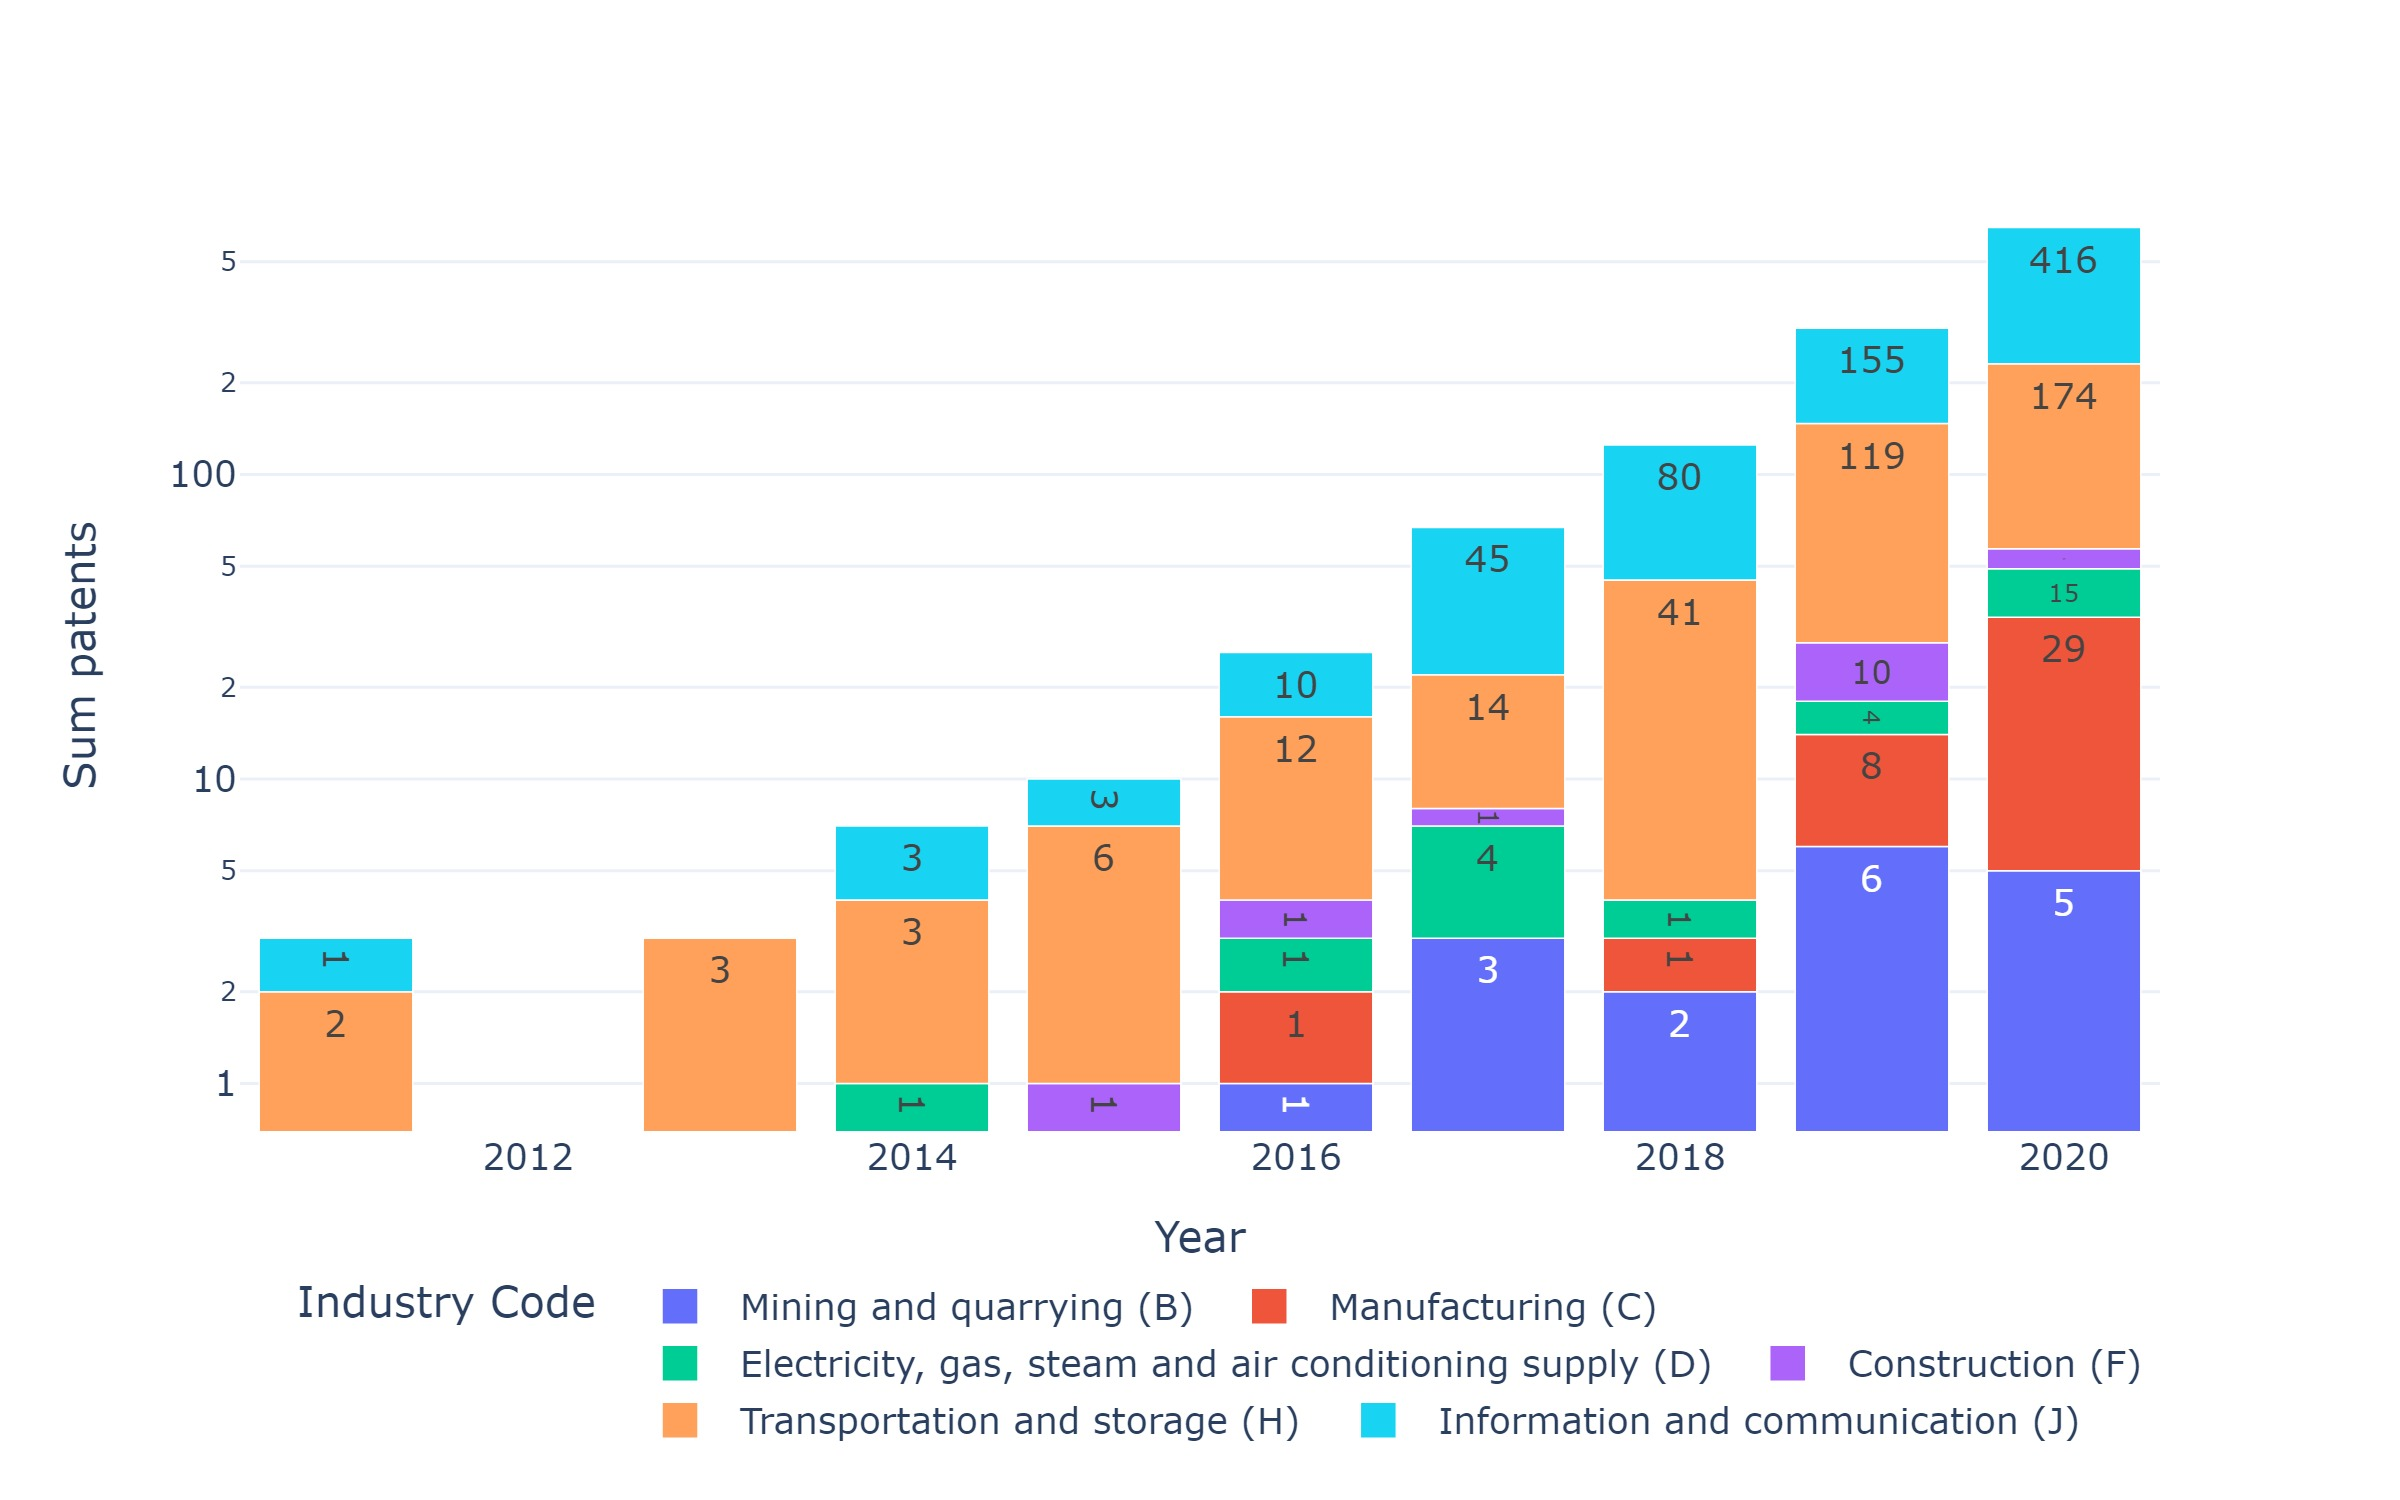
\includegraphics{rieg2023_files/figure-pdf/fig-sum-patents-retrieved-output-1.jpeg}

}

\caption{\label{fig-sum-patents-retrieved}Number of patents retrieved
for each industry and year - log scale}

\end{figure}

As each industry's patent application counts as well as the SBS data
have been retrieved for multiple years, the collected data comprises a
time-series. As shown in Figure~\ref{fig-untransformed-data-example},
data on SBS indicators (blue) as well as the number of patents retrieved
each year (red) clearly does not exhibit stationarity. In order to
account for any trends, the collected data is transformed using linear
detrending method. This is done by utilizing SciPy's detrending method
(\citeproc{ref-virtanen_scipy_2020}{Virtanen et al., 2020}), which fits
a linear least-squares regression to the data and subtracts the
resulting trend of the regression line from the data
(\citeproc{ref-the_scipy_community_scipysignaldetrend_2023}{The SciPy
community, 2023}). Note that other detrending options, such as
logarithmic transformation or differencing have been considered but
deemed insufficient. Logarithmic transformation is not applicable as the
data contains zero values. While there are methods to circumvent this,
for example taking the logarithm \(log(x+1)\), this would lead to
non-null values where null values are expected to control for variance
in the endogenous variable in the absence of patent counts. Furthermore,
as seen in Figure~\ref{fig-untransformed-data-example}, many data series
exhibit a continuous positive or negative trend (lack of fluctuation).
In this case, differencing would merely reverse the trend, and
logarithmic detrending would lead to a compression of the y-scale.
Resulting data transformed by either of these methods, however, would
still exhibit a definite trend. The resulting data, of which an example
is shown in Figure~\ref{fig-transformed-data-example}, is then used for
the regression analyses.

\begin{figure}[H]

{\centering 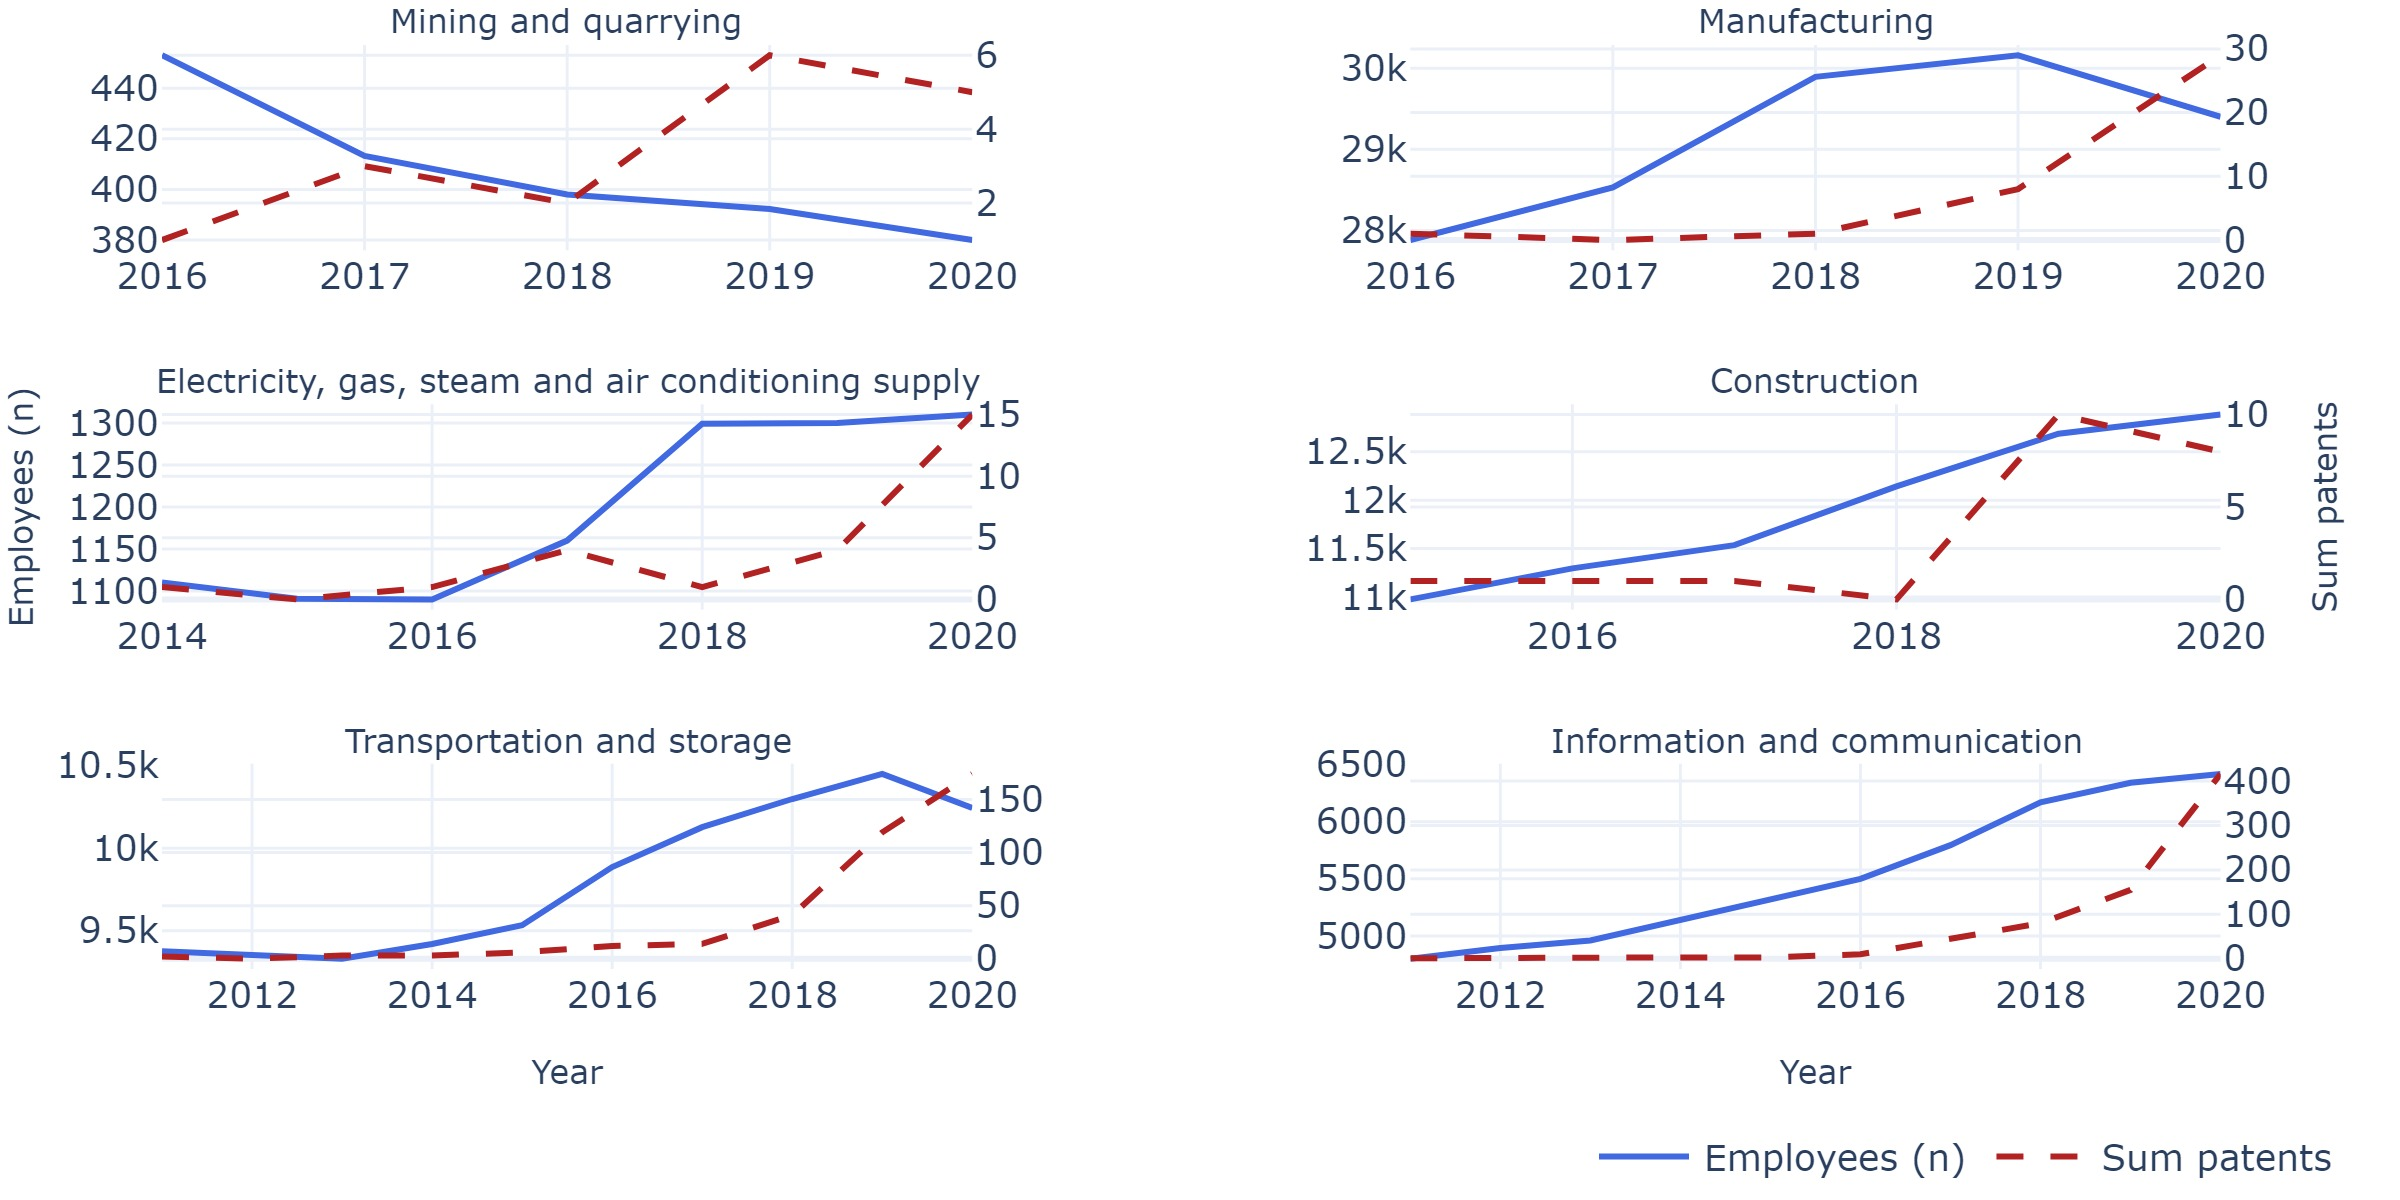
\includegraphics{rieg2023_files/figure-pdf/fig-untransformed-data-example-output-1.jpeg}

}

\caption{\label{fig-untransformed-data-example}Example of untransformed
data for all Industries and NACE Code `Number of Employees' plotted over
years}

\end{figure}

\begin{figure}[H]

{\centering 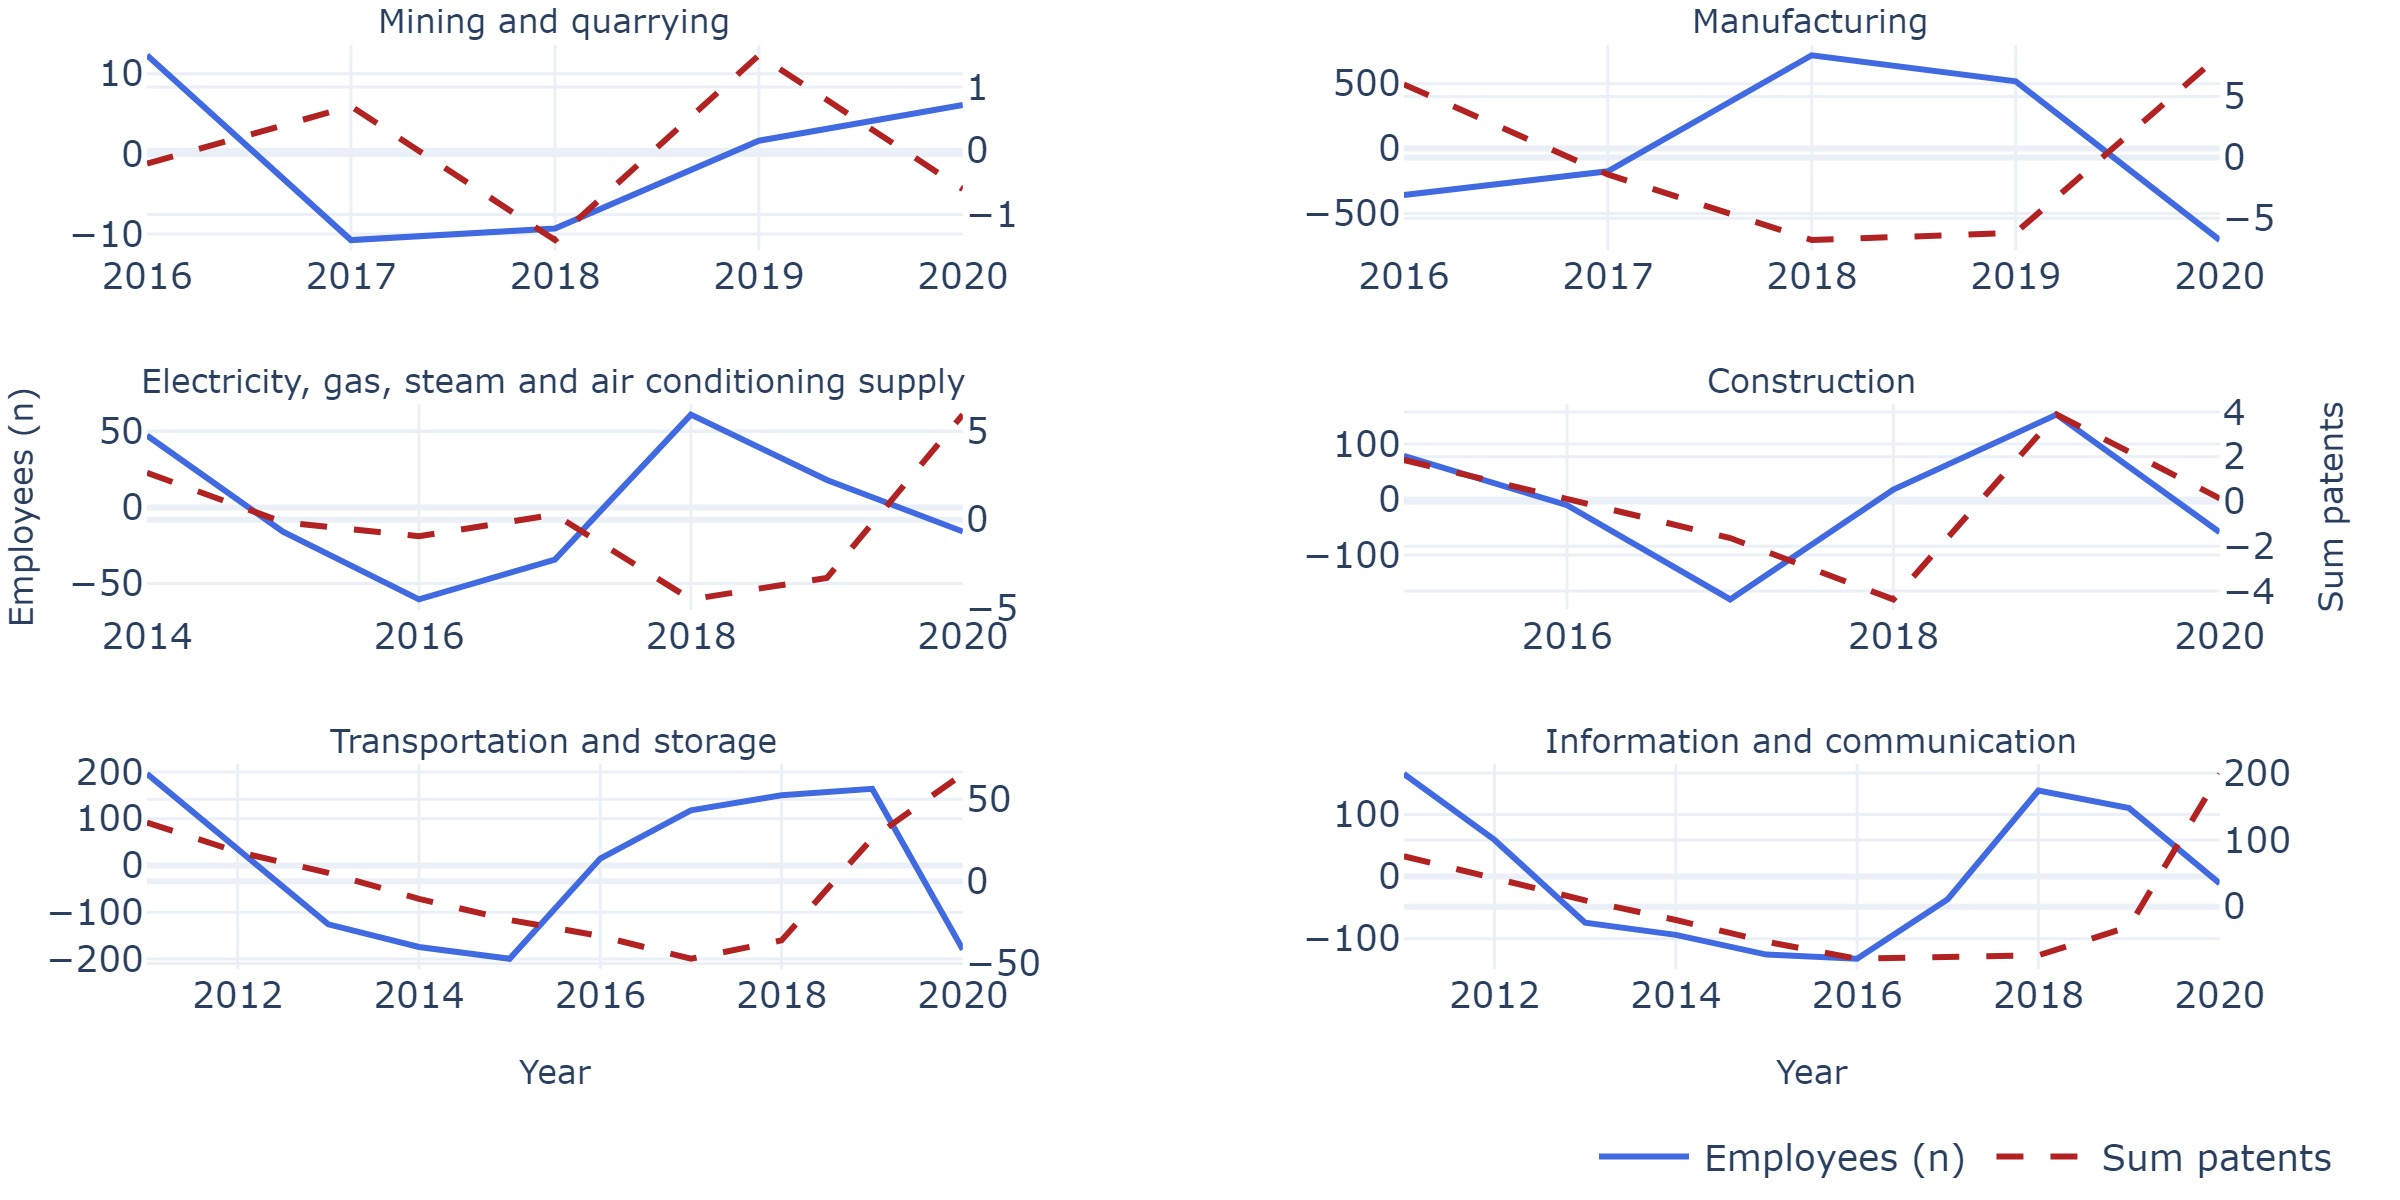
\includegraphics{rieg2023_files/figure-pdf/fig-transformed-data-example-output-1.jpeg}

}

\caption{\label{fig-transformed-data-example}Example of linear detrended
data for all Industries and NACE Code `Number of Employees' plotted over
years}

\end{figure}

Because data has been linearly detrended, to account for any remaining
trend left in the data, the control variable ``Year'' is added to the
regression analyses. This is done to ensure that any remaining trend in
the data is accounted for and does not bias the regression results.
Furthermore, the control variable ``Year'' is also added to the
regression analyses to account for any time dependent macroeconomic
effects that may have affected the chosen economic indicators but are
not considered in the model. Lastly, note that the SBS data contains one
economic indicator, gross value added per employee, that is denoted in
each year's currency value. The (monetary) value has not been adjusted
for inflation, as any trend in the data has been already removed by the
linear detrending method.

\subsection{Model}\label{sec-model}

This research aims to answer the question of how innovation in AI across
industries impact labor conditions. To answer this question, a multiple
linear regression model is used. For each industry, the number of
patents retrieved for each year is used as the exogenous variable to
explain the endogenous variables, which are the chosen economic
indicators. Given five economic indicators across 6 industries, 30
regressions are modeled. The relationship between the number of patents
and the chosen economic indicators are assumed to be linear. While other
relationships may be plausible too, given the small sample size, the
assumption of linearity is made to ensure against possible overfitting
(see Section~\ref{sec-limitations}).

\subsection{Hypotheses}\label{sec-hypotheses}

To determine whether a relationship between the number of patents and
the chosen economic indicators exists, the following hypotheses are
tested. Given a standard multiple linear regression model of the form
\(\hat{y}_{i,j} = \beta_0 + \beta_1x_i + \beta_2x_t\), where
\(\hat{y}=\text{esitmated response, }i=\text{industry, }j=\text{economic indicator }\text{and }t=\text{time}\).
The coefficient \(\beta_1\) is assumed to be \(0\). Specifically, the
following five hypotheses are tested.

\begin{align}
H_{0, i, j}: \beta_1 = 0\text{ for }j=e=\text{number of enterprises, } i\in\{B, C, D, F, H, J\} \\
H_{0, i, j}: \beta_1 = 0\text{ for }j=L=\text{number of employees, } i\in\{B, C, D, F, H, J\}\\
H_{0, i, j}: \beta_1 = 0\text{ for }j=l=\text{wage adjusted labor productivity, } i\in\{B, C, D, F, H, J\}\\
H_{0, i, j}: \beta_1 = 0\text{ for }j=v=\text{gross value added per employee, } i\in\{B, C, D, F, H, J\}\\
H_{0, i, j}: \beta_1 = 0\text{ for }j=c=\text{personnel costs in production, } i\in\{B, C, D, F, H, J\}
\end{align}

\section{Results}\label{sec-results}

The following section presents the main findings from the regression
analyses. Results are summarized by industry, allowing a sectional
comparison of patent counts' influence on economic indicators within an
industry. Note that detailed data about regression results as well as
tests for multiple regression assumptions can be found in the
\nameref{sec-appendix} in Table~\ref{tbl-summary-reg-results-b} to
Table~\ref{tbl-summary-reg-results-j}.

\setstretch{1}

\phantomsection\label{tbl-regression-results-ind-b}
\begin{longtable}[]{@{}
  >{\raggedright\arraybackslash}p{(\columnwidth - 10\tabcolsep) * \real{0.1404}}
  >{\raggedright\arraybackslash}p{(\columnwidth - 10\tabcolsep) * \real{0.1667}}
  >{\raggedright\arraybackslash}p{(\columnwidth - 10\tabcolsep) * \real{0.1491}}
  >{\raggedright\arraybackslash}p{(\columnwidth - 10\tabcolsep) * \real{0.1667}}
  >{\raggedright\arraybackslash}p{(\columnwidth - 10\tabcolsep) * \real{0.1754}}
  >{\raggedright\arraybackslash}p{(\columnwidth - 10\tabcolsep) * \real{0.2018}}@{}}
\caption{\label{tbl-regression-results-ind-b}Regression results - Mining
and Quarrying (B)}\tabularnewline
\toprule\noalign{}
\begin{minipage}[b]{\linewidth}\raggedright
\end{minipage} & \begin{minipage}[b]{\linewidth}\raggedright
Enterprises (n)
\end{minipage} & \begin{minipage}[b]{\linewidth}\raggedright
Employees (n)
\end{minipage} & \begin{minipage}[b]{\linewidth}\raggedright
Labor prod. (\%)
\end{minipage} & \begin{minipage}[b]{\linewidth}\raggedright
GVA/employee (€)
\end{minipage} & \begin{minipage}[b]{\linewidth}\raggedright
Personnel costs (\%)
\end{minipage} \\
\midrule\noalign{}
\endfirsthead
\toprule\noalign{}
\begin{minipage}[b]{\linewidth}\raggedright
\end{minipage} & \begin{minipage}[b]{\linewidth}\raggedright
Enterprises (n)
\end{minipage} & \begin{minipage}[b]{\linewidth}\raggedright
Employees (n)
\end{minipage} & \begin{minipage}[b]{\linewidth}\raggedright
Labor prod. (\%)
\end{minipage} & \begin{minipage}[b]{\linewidth}\raggedright
GVA/employee (€)
\end{minipage} & \begin{minipage}[b]{\linewidth}\raggedright
Personnel costs (\%)
\end{minipage} \\
\midrule\noalign{}
\endhead
\bottomrule\noalign{}
\endlastfoot
const & 0.0000 & 0.0000 & -0.0000 & -3878292.0523 & 0.0000 \\
& (119814.6603) & (8940.2460) & (32619.9298) & (20665152.7595) &
(998.5155) \\
Sum patents & -88.6471 & 0.3627 & -8.1451 & -1340.9907 & 0.6451 \\
& (83.1388) & (6.2036) & (22.6348) & (14778.9277) & (0.6929) \\
Year & -0.0000 & -0.0000 & 0.0000 & 1921.6113 & -0.0000 \\
& (59.3730) & (4.4302) & (16.1645) & (10239.1414) & (0.4948) \\
R-squared & 0.3624 & 0.0017 & 0.0608 & 0.0411 & 0.3024 \\
R-squared Adj. & -0.2751 & -0.9966 & -0.8784 & -1.8766 & -0.3952 \\
\end{longtable}

\vspace{-1.5em}\setstretch{1}\begin{flushleft}\footnotesize\textit{* p < 0.1, ** p < 0.05, *** p < 0.01. Standard errors in parentheses.}\end{flushleft}\setstretch{1.5}

\setstretch{1.5}

For patents classified as industry ``Mining and Quarrying'' (NACE code
``B''), depicted in Table~\ref{tbl-regression-results-ind-b}, the
regression results show no significant relation between the sum of
patents retrieved for each year and the chosen indicators. Furthermore,
the control variable ``Year'', too, does not exhibit any significant
relationships with the economic indicators. It should be noted, however,
that the number of patents retrieved for this industry is very low.
While, as discussed in \nameref{sec-data-acquisition}, industries for
which patents were retrieved in fewer than five years were eliminated
from the data, for Mining and Quarrying only 17 patents in five years
were retrieved. As a result, the nullhypotheses
\(H_{0, i, j}\text{ for }j\in \{e, L, l, v, c\}, i=B\) are not rejected.

\setstretch{1}

\phantomsection\label{tbl-regression-results-ind-c}
\begin{longtable}[]{@{}
  >{\raggedright\arraybackslash}p{(\columnwidth - 10\tabcolsep) * \real{0.1404}}
  >{\raggedright\arraybackslash}p{(\columnwidth - 10\tabcolsep) * \real{0.1667}}
  >{\raggedright\arraybackslash}p{(\columnwidth - 10\tabcolsep) * \real{0.1491}}
  >{\raggedright\arraybackslash}p{(\columnwidth - 10\tabcolsep) * \real{0.1667}}
  >{\raggedright\arraybackslash}p{(\columnwidth - 10\tabcolsep) * \real{0.1754}}
  >{\raggedright\arraybackslash}p{(\columnwidth - 10\tabcolsep) * \real{0.2018}}@{}}
\caption{\label{tbl-regression-results-ind-c}Regression results -
Manufacturing (C)}\tabularnewline
\toprule\noalign{}
\begin{minipage}[b]{\linewidth}\raggedright
\end{minipage} & \begin{minipage}[b]{\linewidth}\raggedright
Enterprises (n)
\end{minipage} & \begin{minipage}[b]{\linewidth}\raggedright
Employees (n)
\end{minipage} & \begin{minipage}[b]{\linewidth}\raggedright
Labor prod. (\%)
\end{minipage} & \begin{minipage}[b]{\linewidth}\raggedright
GVA/employee (€)
\end{minipage} & \begin{minipage}[b]{\linewidth}\raggedright
Personnel costs (\%)
\end{minipage} \\
\midrule\noalign{}
\endfirsthead
\toprule\noalign{}
\begin{minipage}[b]{\linewidth}\raggedright
\end{minipage} & \begin{minipage}[b]{\linewidth}\raggedright
Enterprises (n)
\end{minipage} & \begin{minipage}[b]{\linewidth}\raggedright
Employees (n)
\end{minipage} & \begin{minipage}[b]{\linewidth}\raggedright
Labor prod. (\%)
\end{minipage} & \begin{minipage}[b]{\linewidth}\raggedright
GVA/employee (€)
\end{minipage} & \begin{minipage}[b]{\linewidth}\raggedright
Personnel costs (\%)
\end{minipage} \\
\midrule\noalign{}
\endhead
\bottomrule\noalign{}
\endlastfoot
const & 0.0000 & 0.0000 & -0.0000 & -0.0000 & 0.0000 \\
& (15775939.2113) & (161822.0105) & (554.4693) & (306669.6590) &
(133.4932) \\
Sum patents & -14.6066 & -82.4888** & -0.1300 & -203.3126** & 0.0400 \\
& (1778.5677) & (18.2437) & (0.0625) & (34.5737) & (0.0150) \\
Year & -0.0000 & -0.0000 & 0.0000 & 0.0000 & -0.0000 \\
& (7817.6092) & (80.1893) & (0.2748) & (151.9671) & (0.0662) \\
R-squared & 0.0000 & 0.9109 & 0.6839 & 0.9453 & 0.7790 \\
R-squared Adj. & -0.9999 & 0.8218 & 0.3677 & 0.8907 & 0.5580 \\
\end{longtable}

\vspace{-1.5em}\setstretch{1}\begin{flushleft}\footnotesize\textit{* p < 0.1, ** p < 0.05, *** p < 0.01. Standard errors in parentheses.}\end{flushleft}\setstretch{1.5}

\setstretch{1.5}

For patents classified as industry ``Manufacturing'' (NACE code ``C''),
depicted in Table~\ref{tbl-regression-results-ind-c}, the regression
results show a statistically significant negative relationship between
the number of retrieved patents and the number of employees within the
Manufacturing sector (coef. -82.489, SE 18.243`). In particular, the
regression result's coefficient estimates a decrease of 82.489 employees
for each additional patent retrieved.\footnote{Note that while the
  coefficient's implications are mentioned, this merely refers to the
  slope of the regression line and should not be interpreted as valid
  result with real-world implications. The regression model is not
  intended to be used for prediction.} Furthermore, the control variable
``Year'' does not exhibit a statistically significant relationship with
the number of employees (coef. 0). The adjusted \(R^2\) of 0.82
indicates a high ratio of explainability for the model.

While there are no statistically significant relations between the
number of patents retrieved and the number of enterprises, wage adjusted
labor productivity (labor prod.) and the percentage of personnel costs
in production, the relationship between the number of patents and the
gross value added per employee is statistically significant and negative
(coef. -203.313, SE 34.574) with an adjusted \(R^2\) of 0.89. Lastly, it
should be noted that the control variable does not exhibit a
statistically significant relationship with any of the economic
indicators. As a result, the nullhypotheses
\(H_{0, i, j}\text{ for }j\in \{L, v\}, i=C\) are rejected and
\(H_{0, i, j}\text{ for }j\in \{e, l, c\}, i=C\) cannot be rejected.

\setstretch{1}

\phantomsection\label{tbl-regression-results-ind-d}
\begin{longtable}[]{@{}
  >{\raggedright\arraybackslash}p{(\columnwidth - 10\tabcolsep) * \real{0.1404}}
  >{\raggedright\arraybackslash}p{(\columnwidth - 10\tabcolsep) * \real{0.1667}}
  >{\raggedright\arraybackslash}p{(\columnwidth - 10\tabcolsep) * \real{0.1491}}
  >{\raggedright\arraybackslash}p{(\columnwidth - 10\tabcolsep) * \real{0.1667}}
  >{\raggedright\arraybackslash}p{(\columnwidth - 10\tabcolsep) * \real{0.1754}}
  >{\raggedright\arraybackslash}p{(\columnwidth - 10\tabcolsep) * \real{0.2018}}@{}}
\caption{\label{tbl-regression-results-ind-d}Regression results -
Electricity, gas, steam and air conditioning supply (D)}\tabularnewline
\toprule\noalign{}
\begin{minipage}[b]{\linewidth}\raggedright
\end{minipage} & \begin{minipage}[b]{\linewidth}\raggedright
Enterprises (n)
\end{minipage} & \begin{minipage}[b]{\linewidth}\raggedright
Employees (n)
\end{minipage} & \begin{minipage}[b]{\linewidth}\raggedright
Labor prod. (\%)
\end{minipage} & \begin{minipage}[b]{\linewidth}\raggedright
GVA/employee (€)
\end{minipage} & \begin{minipage}[b]{\linewidth}\raggedright
Personnel costs (\%)
\end{minipage} \\
\midrule\noalign{}
\endfirsthead
\toprule\noalign{}
\begin{minipage}[b]{\linewidth}\raggedright
\end{minipage} & \begin{minipage}[b]{\linewidth}\raggedright
Enterprises (n)
\end{minipage} & \begin{minipage}[b]{\linewidth}\raggedright
Employees (n)
\end{minipage} & \begin{minipage}[b]{\linewidth}\raggedright
Labor prod. (\%)
\end{minipage} & \begin{minipage}[b]{\linewidth}\raggedright
GVA/employee (€)
\end{minipage} & \begin{minipage}[b]{\linewidth}\raggedright
Personnel costs (\%)
\end{minipage} \\
\midrule\noalign{}
\endhead
\bottomrule\noalign{}
\endlastfoot
const & 0.0000 & 0.0000 & -0.0000 & 0.0000 & 0.0000 \\
& (7090398.8328) & (19752.8953) & (2819.3693) & (1493538.8451) &
(103.5974) \\
Sum patents & -2148.9258 & -3.4280 & 1.4361 & 581.8882 & 0.0439 \\
& (2160.2744) & (6.0182) & (0.8590) & (455.0454) & (0.0164) \\
Year & -0.0000 & -0.0000 & 0.0000 & -0.0000 & -0.0000 \\
& (3515.3175) & (9.7932) & (1.3978) & (740.4750) & (0.0513) \\
R-squared & 0.1983 & 0.0750 & 0.4113 & 0.2902 & 0.8780 \\
R-squared Adj. & -0.2025 & -0.3875 & 0.1170 & -0.0647 & 0.6341 \\
\end{longtable}

\vspace{-1.5em}\setstretch{1}\begin{flushleft}\footnotesize\textit{* p < 0.1, ** p < 0.05, *** p < 0.01. Standard errors in parentheses.}\end{flushleft}\setstretch{1.5}

\phantomsection\label{tbl-regression-results-ind-f}
\begin{longtable}[]{@{}
  >{\raggedright\arraybackslash}p{(\columnwidth - 10\tabcolsep) * \real{0.1404}}
  >{\raggedright\arraybackslash}p{(\columnwidth - 10\tabcolsep) * \real{0.1667}}
  >{\raggedright\arraybackslash}p{(\columnwidth - 10\tabcolsep) * \real{0.1491}}
  >{\raggedright\arraybackslash}p{(\columnwidth - 10\tabcolsep) * \real{0.1667}}
  >{\raggedright\arraybackslash}p{(\columnwidth - 10\tabcolsep) * \real{0.1754}}
  >{\raggedright\arraybackslash}p{(\columnwidth - 10\tabcolsep) * \real{0.2018}}@{}}
\caption{\label{tbl-regression-results-ind-f}Regression results -
Construction (F)}\tabularnewline
\toprule\noalign{}
\begin{minipage}[b]{\linewidth}\raggedright
\end{minipage} & \begin{minipage}[b]{\linewidth}\raggedright
Enterprises (n)
\end{minipage} & \begin{minipage}[b]{\linewidth}\raggedright
Employees (n)
\end{minipage} & \begin{minipage}[b]{\linewidth}\raggedright
Labor prod. (\%)
\end{minipage} & \begin{minipage}[b]{\linewidth}\raggedright
GVA/employee (€)
\end{minipage} & \begin{minipage}[b]{\linewidth}\raggedright
Personnel costs (\%)
\end{minipage} \\
\midrule\noalign{}
\endfirsthead
\toprule\noalign{}
\begin{minipage}[b]{\linewidth}\raggedright
\end{minipage} & \begin{minipage}[b]{\linewidth}\raggedright
Enterprises (n)
\end{minipage} & \begin{minipage}[b]{\linewidth}\raggedright
Employees (n)
\end{minipage} & \begin{minipage}[b]{\linewidth}\raggedright
Labor prod. (\%)
\end{minipage} & \begin{minipage}[b]{\linewidth}\raggedright
GVA/employee (€)
\end{minipage} & \begin{minipage}[b]{\linewidth}\raggedright
Personnel costs (\%)
\end{minipage} \\
\midrule\noalign{}
\endhead
\bottomrule\noalign{}
\endlastfoot
const & -0.0000 & -0.0000 & -0.0000 & 0.0000 & 0.0000 \\
& (21172494.6121) & (58291.4313) & (659.6442) & (476813.8504) &
(117.8279) \\
Sum patents & 9252.7110 & 23.4435 & -0.2356 & 16.5014 & 0.0191 \\
& (6911.8456) & (19.0295) & (0.2153) & (155.6578) & (0.0385) \\
Year & 0.0000 & 0.0000 & 0.0000 & -0.0000 & -0.0000 \\
& (10494.4174) & (28.8929) & (0.3270) & (236.3389) & (0.0584) \\
R-squared & 0.3740 & 0.3359 & 0.2851 & 0.0037 & 0.0756 \\
R-squared Adj. & -0.0434 & -0.1068 & -0.1915 & -0.6604 & -0.5407 \\
\end{longtable}

\vspace{-1.5em}\setstretch{1}\begin{flushleft}\footnotesize\textit{* p < 0.1, ** p < 0.05, *** p < 0.01. Standard errors in parentheses.}\end{flushleft}\setstretch{1.5}

\setstretch{1.5}

For patents classified as industry ``Electricity, gas, steam and air
conditioning supply'' (NACE code ``D''), depicted in
Table~\ref{tbl-regression-results-ind-d}, as well as for patents falling
into the ``Construction'' (``F'') industry in
Table~\ref{tbl-regression-results-ind-f}, the regression results show no
statistically significant relationship between the number of patents
retrieved and the chosen economic indicators. The control variable
``Year'', too, does not exhibit a statistically significant relationship
with the chosen indicators. Furthermore, the adjusted \(R^2\) is very
low (and often even negative) across all dependent variables, indicating
no explanatory power of the model. Therefore, the nullhypotheses
\(H_{0, i, j}\text{ for }j\in \{e, L, l v, c\}, i\in\{D, F\}\) cannot be
rejected.

\setstretch{1}

\phantomsection\label{tbl-regression-results-ind-h}
\begin{longtable}[]{@{}
  >{\raggedright\arraybackslash}p{(\columnwidth - 10\tabcolsep) * \real{0.1404}}
  >{\raggedright\arraybackslash}p{(\columnwidth - 10\tabcolsep) * \real{0.1667}}
  >{\raggedright\arraybackslash}p{(\columnwidth - 10\tabcolsep) * \real{0.1491}}
  >{\raggedright\arraybackslash}p{(\columnwidth - 10\tabcolsep) * \real{0.1667}}
  >{\raggedright\arraybackslash}p{(\columnwidth - 10\tabcolsep) * \real{0.1754}}
  >{\raggedright\arraybackslash}p{(\columnwidth - 10\tabcolsep) * \real{0.2018}}@{}}
\caption{\label{tbl-regression-results-ind-h}Regression results -
Transportation and storage (H)}\tabularnewline
\toprule\noalign{}
\begin{minipage}[b]{\linewidth}\raggedright
\end{minipage} & \begin{minipage}[b]{\linewidth}\raggedright
Enterprises (n)
\end{minipage} & \begin{minipage}[b]{\linewidth}\raggedright
Employees (n)
\end{minipage} & \begin{minipage}[b]{\linewidth}\raggedright
Labor prod. (\%)
\end{minipage} & \begin{minipage}[b]{\linewidth}\raggedright
GVA/employee (€)
\end{minipage} & \begin{minipage}[b]{\linewidth}\raggedright
Personnel costs (\%)
\end{minipage} \\
\midrule\noalign{}
\endfirsthead
\toprule\noalign{}
\begin{minipage}[b]{\linewidth}\raggedright
\end{minipage} & \begin{minipage}[b]{\linewidth}\raggedright
Enterprises (n)
\end{minipage} & \begin{minipage}[b]{\linewidth}\raggedright
Employees (n)
\end{minipage} & \begin{minipage}[b]{\linewidth}\raggedright
Labor prod. (\%)
\end{minipage} & \begin{minipage}[b]{\linewidth}\raggedright
GVA/employee (€)
\end{minipage} & \begin{minipage}[b]{\linewidth}\raggedright
Personnel costs (\%)
\end{minipage} \\
\midrule\noalign{}
\endhead
\bottomrule\noalign{}
\endlastfoot
const & 0.0000 & 0.0000 & 0.0000 & 0.0000 & 0.0000 \\
& (3846872.7673) & (39250.0211) & (706.0715) & (376987.6682) &
(124.3979) \\
Sum patents & 594.7790*** & -0.4540 & -0.1021** & -33.0649* &
0.0156** \\
& (159.0156) & (1.6225) & (0.0292) & (15.5833) & (0.0051) \\
Year & -0.0000 & -0.0000 & -0.0000 & -0.0000 & -0.0000 \\
& (1908.6425) & (19.4741) & (0.3503) & (187.0441) & (0.0617) \\
R-squared & 0.6665 & 0.0111 & 0.6362 & 0.3914 & 0.5673 \\
R-squared Adj. & 0.5712 & -0.2715 & 0.5322 & 0.2175 & 0.4436 \\
\end{longtable}

\vspace{-1.5em}\setstretch{1}\begin{flushleft}\footnotesize\textit{* p < 0.1, ** p < 0.05, *** p < 0.01. Standard errors in parentheses.}\end{flushleft}\setstretch{1.5}

\setstretch{1.5}

The regression models between number of patents allocated to the
transportation and storage industry (H) and the chosen endogenous
variables, depicted in Table~\ref{tbl-regression-results-ind-h}, show a
number of statistically significant relationships. First, the number of
filed patents is statistically significant in predicting the number of
enterprises present in any given year. The coefficient of 94.78 (SE
159.016) implies a positive relationship between the number of AI
patents and the number of Enterprises. The control variable remains
statistically insignificant. This holds also true for the remaining
indicators modeled within the transportation and storage industry. The
adjusted \(R^2\) of 0.57 indicates that over 50\% of the predictors'
variance is explained by the model. No statistically significant
relationship can be reported between the industries retrieved annual
patent counts and the number of employees and gross value added per
employee. However, wage adjusted labor productivity exhibits a
statistically negative relationship with a coefficient of -0.102 and a
standard error of 0.029 (Adj. \(R^2\) 0.532). The same relationship
occurs for the percentage of personnel costs in production which is
found to be significantly positively related to the number of patents
filed (coef. 0.005, SE 0.005). To conclude, hypotheses
\(H_{0, i, j}\text{ for }j\in \{e, l, c\}, i=H\) are rejected and
\(H_{0, i, j}\text{ for }j\in \{L, v\}, i=H\) cannot be rejected.

\setstretch{1}

\phantomsection\label{tbl-regression-results-ind-j}
\begin{longtable}[]{@{}
  >{\raggedright\arraybackslash}p{(\columnwidth - 10\tabcolsep) * \real{0.1404}}
  >{\raggedright\arraybackslash}p{(\columnwidth - 10\tabcolsep) * \real{0.1667}}
  >{\raggedright\arraybackslash}p{(\columnwidth - 10\tabcolsep) * \real{0.1491}}
  >{\raggedright\arraybackslash}p{(\columnwidth - 10\tabcolsep) * \real{0.1667}}
  >{\raggedright\arraybackslash}p{(\columnwidth - 10\tabcolsep) * \real{0.1754}}
  >{\raggedright\arraybackslash}p{(\columnwidth - 10\tabcolsep) * \real{0.2018}}@{}}
\caption{\label{tbl-regression-results-ind-j}Regression results -
Information and communication (J)}\tabularnewline
\toprule\noalign{}
\begin{minipage}[b]{\linewidth}\raggedright
\end{minipage} & \begin{minipage}[b]{\linewidth}\raggedright
Enterprises (n)
\end{minipage} & \begin{minipage}[b]{\linewidth}\raggedright
Employees (n)
\end{minipage} & \begin{minipage}[b]{\linewidth}\raggedright
Labor prod. (\%)
\end{minipage} & \begin{minipage}[b]{\linewidth}\raggedright
GVA/employee (€)
\end{minipage} & \begin{minipage}[b]{\linewidth}\raggedright
Personnel costs (\%)
\end{minipage} \\
\midrule\noalign{}
\endfirsthead
\toprule\noalign{}
\begin{minipage}[b]{\linewidth}\raggedright
\end{minipage} & \begin{minipage}[b]{\linewidth}\raggedright
Enterprises (n)
\end{minipage} & \begin{minipage}[b]{\linewidth}\raggedright
Employees (n)
\end{minipage} & \begin{minipage}[b]{\linewidth}\raggedright
Labor prod. (\%)
\end{minipage} & \begin{minipage}[b]{\linewidth}\raggedright
GVA/employee (€)
\end{minipage} & \begin{minipage}[b]{\linewidth}\raggedright
Personnel costs (\%)
\end{minipage} \\
\midrule\noalign{}
\endhead
\bottomrule\noalign{}
\endlastfoot
const & -0.0000 & 0.0000 & 0.0000 & 0.0000 & -0.0000 \\
& (2195739.8894) & (27234.7248) & (438.8221) & (225189.9648) &
(69.7770) \\
Sum patents & 2.9806 & 0.2962 & 0.0325*** & 22.0818*** & -0.0028* \\
& (37.9587) & (0.4708) & (0.0076) & (3.8930) & (0.0012) \\
Year & 0.0000 & -0.0000 & -0.0000 & -0.0000 & 0.0000 \\
& (1089.4258) & (13.5126) & (0.2177) & (111.7290) & (0.0346) \\
R-squared & 0.0009 & 0.0535 & 0.7242 & 0.8213 & 0.4411 \\
R-squared Adj. & -0.2846 & -0.2169 & 0.6454 & 0.7703 & 0.2815 \\
\end{longtable}

\vspace{-1.5em}\setstretch{1}\begin{flushleft}\footnotesize\textit{* p < 0.1, ** p < 0.05, *** p < 0.01. Standard errors in parentheses.}\end{flushleft}\setstretch{1.5}

\setstretch{1.5}

Lastly, the regression models' results, as shown in
Table~\ref{tbl-regression-results-ind-j}, yield similar results for the
information and communication industry (NACE code ``J''). Here no
significant relationship was found between the number of patents
retrieved and the number of enterprises, with a negative adjusted
\(R^2\), showing independent variables yielding no explanatory power
over the dependent variable. The same results can be reported for the
model on the number of employees. However, the number of patents
retrieved is found to be significantly and positively related to wage
adjusted labor productivity (coef. 0.033, SE 0.008) and results show an
adjusted \(R^2\) of 0.645. The same relationship can be reported for the
gross value added per employee (coef. 22.082, SE 3.893), which yields
the highest adjusted \(R^2\) (0.770) of all models in this analysis. The
number of AI patents does not significantly explain the percentage share
of personnel costs in production. Therefore,
\(H_{0, i, j}\text{ for }j\in \{l, v\}, i=J\) are rejected and
\(H_{0, i, j}\text{ for }j\in \{e, L, c\}, i=J\) are accepted.

In summary, the models' results paint a rather mixed picture with the
majority of models tested showing statistically insignificant
relationships between the number of AI patents retrieved for an
industry, and the chosen economic indicators reported within each
industry. Only seven out of the 30 models tested exhibit statistically
significant relationships. The results are further exacerbated, when one
considers the fact that the chance of a rare event occurring increases
with repeated exposure to that probability.\footnote{A good analogy
  would be that the chance of winning the lottery increases with
  repeated playing. Or that the chance of rolling a six on a die is more
  likely in four rolls than in one roll.} A common method to correct for
the possibility of false positives is the Bonferroni Correction
(\citeproc{ref-mittelhammer_econometric_2000}{Mittelhammer et al., 2000,
p. 73f}.). Given the above chosen \(\alpha\)-level of 0.05, the
Bonferroni Correction counterbalances the increased likelihood of rare
events (in this case, the Type I error) occurring when exposed to a
plurality of situations in which they could occur (e.g., running a
multitude of regressions). The Bonferroni Correction is calculated by
dividing the chosen \(\alpha\)-level by the number of tests conducted.
In this case, the Bonferroni Correction would be
\(\frac{0.05}{30}=0.00167\). This means that accounting for the number
of models evaluated in this section, adjusted \(\alpha\)-level would
need to be set to 0.00167 to diminish the chance of false positives in
the models' results.

\setstretch{1}

\phantomsection\label{tbl-pvalues}
\begin{longtable}[]{@{}lllllll@{}}
\caption{\label{tbl-pvalues}Retrieved significant p values for
coefficients of number of patents by industry and
indicator}\tabularnewline
\toprule\noalign{}
Indicator & B & C & D & F & H & J \\
\midrule\noalign{}
\endfirsthead
\toprule\noalign{}
Indicator & B & C & D & F & H & J \\
\midrule\noalign{}
\endhead
\bottomrule\noalign{}
\endlastfoot
Employees (n) & & 0.04559 & & & & \\
Enterprises (n) & & & & & 0.00726 & \\
GVA/employee (€) & & 0.02772 & & & & 0.00076 \\
Labor prod. (\%) & & & & & 0.01001 & 0.00362 \\
Personnel costs (\%) & & & & & 0.01913 & \\
\end{longtable}

\vspace{-1.5em}\setstretch{1}\begin{flushleft}\hspace{3cm}\footnotesize\textit{Note: p values for regression models smaller than 0.05.}\end{flushleft}\setstretch{1.5}

\setstretch{1.5}

Table~\ref{tbl-pvalues}, depicts only the number of patents'
coefficient's p values that lie beneath the unadjusted \(\alpha\)
threshold of 0.05. When considering the adjusted \(\alpha\) value of
0.00167, one can see that merely one regression result's p value
fulfills the new criterion (wage adjusted labor productivity in industry
J). To conclude, the presented regression results vary in their
significance and explanatory power to such extent, that it is doubtful
in how far relationships, while being statistically significant,
actually exist. Additionally, the Bonferroni Correction shows that the
at least some of the presented results are likely to be false positives.

\section{Discussion}\label{sec-discussion}

\subsection{Implications}\label{sec-implications}

This research aims to answer the question if and how AI innovation
impacts labor. Given the mixed results presented in
Section~\ref{sec-results}, it is difficult to deduce clear implications
of the findings. While there are significant relationships between some
of the numbers of AI patents filed and industries and indicators, the
vast majority depicts - if any - insufficiently strong links between the
main predictor and predicted variable. Furthermore, as discussed in
Section~\ref{sec-results}, when adjusting the p value threshold for the
number of models fitted, only one model out of 30 fulfills this new
threshold. Furthermore, as this research utilized a to some degree novel
approach to assess the relationship between AI innovation and labor, the
absence of significant findings still aids to enrich the current corpus
of literature by providing evidence that the relationship between AI
patents filed and the chosen economic indicators is not as clear as one
might expect. Nevertheless, when looking at between-industry and
between-indicator results, a few interesting findings can be reported.

\setstretch{1}

\phantomsection\label{tbl-pvalues-extended}
\begin{longtable}[]{@{}
  >{\raggedright\arraybackslash}p{(\columnwidth - 16\tabcolsep) * \real{0.2165}}
  >{\raggedright\arraybackslash}p{(\columnwidth - 16\tabcolsep) * \real{0.0515}}
  >{\raggedright\arraybackslash}p{(\columnwidth - 16\tabcolsep) * \real{0.0928}}
  >{\raggedright\arraybackslash}p{(\columnwidth - 16\tabcolsep) * \real{0.0515}}
  >{\raggedright\arraybackslash}p{(\columnwidth - 16\tabcolsep) * \real{0.0515}}
  >{\raggedright\arraybackslash}p{(\columnwidth - 16\tabcolsep) * \real{0.1031}}
  >{\raggedright\arraybackslash}p{(\columnwidth - 16\tabcolsep) * \real{0.1031}}
  >{\raggedright\arraybackslash}p{(\columnwidth - 16\tabcolsep) * \real{0.1753}}
  >{\raggedright\arraybackslash}p{(\columnwidth - 16\tabcolsep) * \real{0.1546}}@{}}
\caption{\label{tbl-pvalues-extended}Significant p values with
coefficient sign, sample size and total number of
patents}\tabularnewline
\toprule\noalign{}
\begin{minipage}[b]{\linewidth}\raggedright
\end{minipage} & \begin{minipage}[b]{\linewidth}\raggedright
B
\end{minipage} & \begin{minipage}[b]{\linewidth}\raggedright
C
\end{minipage} & \begin{minipage}[b]{\linewidth}\raggedright
D
\end{minipage} & \begin{minipage}[b]{\linewidth}\raggedright
F
\end{minipage} & \begin{minipage}[b]{\linewidth}\raggedright
H
\end{minipage} & \begin{minipage}[b]{\linewidth}\raggedright
J
\end{minipage} & \begin{minipage}[b]{\linewidth}\raggedright
Patents (sum)
\end{minipage} & \begin{minipage}[b]{\linewidth}\raggedright
Sample size
\end{minipage} \\
\midrule\noalign{}
\endfirsthead
\toprule\noalign{}
\begin{minipage}[b]{\linewidth}\raggedright
\end{minipage} & \begin{minipage}[b]{\linewidth}\raggedright
B
\end{minipage} & \begin{minipage}[b]{\linewidth}\raggedright
C
\end{minipage} & \begin{minipage}[b]{\linewidth}\raggedright
D
\end{minipage} & \begin{minipage}[b]{\linewidth}\raggedright
F
\end{minipage} & \begin{minipage}[b]{\linewidth}\raggedright
H
\end{minipage} & \begin{minipage}[b]{\linewidth}\raggedright
J
\end{minipage} & \begin{minipage}[b]{\linewidth}\raggedright
Patents (sum)
\end{minipage} & \begin{minipage}[b]{\linewidth}\raggedright
Sample size
\end{minipage} \\
\midrule\noalign{}
\endhead
\bottomrule\noalign{}
\endlastfoot
Employees (n) & & 0.04559 & & & & & 1190.0 & 43.0 \\
Enterprises (n) & & & & & 0.00726* & & 1190.0 & 43.0 \\
GVA/employee (€) & & 0.02772 & & & & 0.00076* & 1187.0 & 42.0 \\
Labor prod. (\%) & & & & & 0.01001 & 0.00362* & 1190.0 & 43.0 \\
Personnel costs (\%) & & & & & 0.01913* & & 1188.0 & 40.0 \\
Patents (sum) & 17 & 39 & 26 & 21 & 374 & 713 & & \\
Sample size & 5 & 5 & 7 & 6 & 10 & 10 & & \\
\end{longtable}

\vspace{-1.5em}\setstretch{1}\begin{flushleft}\footnotesize\textit{Note: p values for regression models smaller than 0.05. * indicates a positive coefficient.}\end{flushleft}\setstretch{1.5}

\setstretch{1.5}

Table~\ref{tbl-pvalues-extended} builds upon Table~\ref{tbl-pvalues} and
depicts the significant regression results from
Section~\ref{sec-results} that fall beneath the unadjusted \(\alpha\)
threshold of 0.05 in conjunction with the sign of the sum of patent's
coefficients (``*'' for a positive coefficient) as well as the total
number of individual patents retrieved by industry and indicator
(``Patents (sum)'') and the sample size by industry and indicator
(``Sample size''). The sum of patents here is the aggregate sum of
individual patents retrieved. The sample size denotes the number of
aggregates that are contained in each group.\footnote{Since patents have
  been aggregated by industry and year, the sample size also depicts the
  number of years for which patent counts have been recorded. Note that
  this does not mean that patents have been retrieved for each year (see
  Section~\ref{sec-preprocessing},
  p.~\pageref{cleaning-missing-values}).} The first cross-industry
finding is that significant relationships have only been found in groups
that lay in the upper half of the total number of patents retrieved.
While for industries B, D and F no statistically significant
relationships were found, these industries also had the lowest number of
total patents retrieved with 17, 26, and 21 respectively. The industries
with the highest number of patents retrieved, C, H and J, in turn all
exhibit at least two statistically significant relationships.
Furthermore, besides wage adjusted labor productivity in industry H
(Transportation and storage), if effects where present in an industry,
they do exhibit the same relationship within one industry. For example,
in industry C (Manufacturing), the significant effects of AI patent
applications on the number of employees, as well as the gross value
added per employee are both negative. While, as discussed in
\nameref{sec-introduction}, automation tends to always displace labor
(whether on a macro or micro level), the displacement of labor, which is
depicted here on an EU-wide industry level, should intuitively relate to
higher marginal productivity per employee and therefore higher gross
value added. However, the results show that the number of employees, as
well as the amount of gross value added per employee decreases with an
increasing number of AI patent applications. This suggests that the
manufacturing industry is contracting with an increased number of AI
patents filed.\footnote{Note that because the data has been detrended
  (see Section~\ref{sec-preprocessing}), statements about the
  regression's coefficients do not reflect the actual trend of an
  industry. Instead, it estimates the effects in the presence of
  stationarity.} Nevertheless, it should be noted that this does not
mean that the manufacturing industry is contracting \emph{because} of
increased AI patent applications. In fact, it may even be the case,
theoretically, that AI patent applications curb the severity of
contraction but that its effects are not strong enough to offset outside
forces.

The opposite holds true for the information and communication industry
(J), which exhibits a positive relationship between AI patent filings
and gross value added per employee as well as wage adjusted labor
productivity. Regarding the gross value added, the positive relationship
was anticipated, and it is surprising that only the information and
communication industry (J) as well as the manufacturing industry (C)
exhibit significant relationships. As automation either displaces labor
or aids labor productivity, one would expect the produced gross value as
a ratio over the number of employees to grow with increased exposure to
any type of technology. However, for the manufacturing industry (C),
this relationship is negative.

To conclude, while there are indications in the results that suggest the
possible existence of a relationship between AI applications and the
chosen economic indicators, more research is needed to verify these
results. For now, the validity of the present results above should be
taken with caution. Neither are there clear patterns in the results
across industries, nor across indicators. One of the few solid
observations from a cross-result view is the fact that results only
appear once the number of total patents filed in an industry crosses a
certain threshold. This does not mean, however, that indicators of
industries, which are not considered in this research, should
necessarily hold significant relationships to the number of filed AI
patents. Rather, it is likely that a higher number of patents helps
averaging out the disproportional effects between each individual
patent. This will be discussed further in the \nameref{sec-limitations}
(Section~\ref{sec-limitations}). For now, the results suggest that the
relationship between AI patent applications and the chosen economic
indicators is not as clear as one might expect.

\subsection{Limitations}\label{sec-limitations}

Given the to some degree novel approach in the data collection process
that this research adopted, a few limitations must be considered to
assess the validity of the presented results above. First, the data
acquisition process. Since patents have been retrieved from the EPO API
via keyword search and not --- like previous research --- via patent
text classification (see \citeproc{ref-mann_benign_2018}{Mann and
Püttmann, 2018}) or occupational classification (see
\citeproc{ref-acemoglu_ai_2020}{Acemoglu et al., 2020a}), the retrieved
patents may not be representative of the actual number of AI patents
filed. For once, keywords used to map a patent's title or abstract to
its industry were only retrieved from the NACE codes' description. While
keywords have been retrieved not only for the overall industry but also
for each group within each division, the keywords extracted from these
descriptions are likely not fully representative for the industry as a
whole. Occupations and tasks within each industry as well as
characteristics of an industry are manifold. Furthermore, a patents
applicable use may not be concealed to one specific industry but rather
to a type of task that occurs across industries or occupations. These
patents have likely not been retrieved and, therefore, lowered the data
quality and size of the data set. In addition, as discussed in
Section~\ref{sec-data-acquisition}, due to language restrictions, only
patents with an application number for the European Patent Office have
been retrieved. While economic data retrieved from Eurostat represents
aggregate country levels, patent applications filed with the EPO are not
necessarily filed with their respective national patent office and vice
versa. In other words, the patents filed with the EPO are not aggregates
of the national patent offices' applications. This is further
exacerbated by the fact that the EPO is not an official institution of
the European Union. While all EU member states are also members of the
EPO, the EPO counts member states that are not in turn members of the
European Union
(\citeproc{ref-european_patent_office_member_nodate}{European Patent
Office, n.d.d}). As it is difficult to assess the origin of a patent,
let alone its geographical applicability, it is likely that the
retrieved patents are not representative of the actual number of AI
patents filed within the EU. Here, patent data on a national level
together with native language keywords would likely yield more precise
results. It may also be the case that some industries tend to file
patent applications generally with national patent offices rather than
the EPO. Assuming that this is the case, it would mean that the
distribution of retrieved patents between industries is biased. Lastly,
the chosen Cooperative Patent Classification (CPC) codes may not capture
all patents that are related to AI. While the CPC codes have been chosen
to be as broad as possible, it is likely that some patents have been
missed. As mentioned in Section~\ref{sec-data-sources}, there are valid
arguments to choose a legal definition of AI on which CPC code selection
is based. However, a legal definition may fail to capture the whole
spectrum of AI technologies, or capture more than what others may
consider to be Artificial Intelligence. Here, the lack of a clear
definition of what AI encapsulates inhibits a precise selection of AI
technologies. Additionally, while a legal definition has been chosen,
there is no precise mapping between the chosen definition and the CPC
codes. As a result, CPC codes have been chosen as good as possible but
may not be a complete set. Even with the same definition of AI, it is
likely that the mapping from the definition to the CPC codes would
differ from person to person as many definitions often leave room for
interpretation. Regarding the CPC codes, it may also be the case that
patent classification codes do not exist for certain technologies yet,
which would inhibit the precision with which patents can be retrieved.

A second limitation regards the nature and characteristics of the patent
applications themselves. More specifically, the date of patent
application does not relate to the date that a patent gains economic
traction. Since patent application is a time consuming process (which,
according to the EPO, takes between three to four years
(\citeproc{ref-european_patent_office_patenting_nodate}{European Patent
Office, n.d.e})), the time a patent becomes economically applicable is
shifted from the time a patent application is filed. Previous research
has incorporated such shifts, or lags, to account for the time delay
between patent application and implementation (see
\citeproc{ref-van_roy_technology_2018}{Van Roy et al., 2018, p. 5}).
This, however, is not necessarily a severe limitation as the number of
patent applications filed serves merely as a proxy for the interest and
innovation in AI applications at any given time. It can be assumed, that
increased inventorship in AI, as approximated by AI related patent
applications, is accompanied by an increased interest in currently
available AI technologies. This, of course, is merely an assumption and
would need to be verified. It would be possible to shift the retrieved
patent data by any given number of years, but as Eurostat's Structural
Business Statistic currently only captures economic activity until 2020,
most retrieved patent applications would have been pushed out of the
data set, making it even smaller. It would be interesting to see future
research, once additional data becomes available, to reproduce a
modified version of this research with retrieved patent applications'
dates being shifted by the average time a patent application takes to be
granted. Furthermore, as pointed out by Trajtenberg
(\citeproc{ref-trajtenberg_penny_1990}{1990}), the plain number of
patent counts disregards the fact that patents do not carry equal
economical weight. That is, the effect which a patent might have on a
market or industry cannot be inferred by the presence of a patent
without incorporating weights. Since this research did not aim to
establish a clear link between patent applications and economic
indicators, but rather used patent applications as a proxy for the
interest in AI, this limitation is of lesser severity. Nevertheless,
weighted patent counts (see \citeproc{ref-van_roy_technology_2018}{Van
Roy et al., 2018, p. 5}) may yield different results as not every patent
application is, first, granted, and second, also of economic value.
There are a variety of weighting methods that may yield better results
in estimating a patent's economic value and impact, such as
forward-citation count, backward-citation count, and number of
non-patent references (\citeproc{ref-bronwyn_h_hall_market_2005}{Bronwyn
H. Hall et al., 2005}; \citeproc{ref-gambardella_value_2008}{Gambardella
et al., 2008}; \citeproc{ref-harhoff_citations_2003}{Harhoff et al.,
2003}; \citeproc{ref-neuhausler_patents_2011}{Neuhäusler et al., 2011};
see \citeproc{ref-squicciarini_measuring_2013}{Squicciarini et al.,
2013}). Lastly, the patent data retrieved from the EPO API does not
contain any information on the patent's country of origin. As mentioned
above, it is almost certain that not all patents have been filed by
EU-based companies or inventors. While some patents carry a company as
the applicant's name, any inventor may file a patent with the European
Patent Office, even if the inventor never intends to make economic use
of the patent in the EPO's jurisdiction. Therefore, it may be the case
that at a significant share of the patents filed with the EPO do not
serve as a proxy for the interest and innovation in AI within the EU but
rather outside it.

A third limitation is the number of data points in the final data set on
which the overall analysis is build. While almost ten thousand patents
have been retrieved from the API, only 4347 were unique in each
industry, and only 1190 patents fulfilled the criteria listed in
\nameref{sec-preprocessing} Section~\ref{sec-preprocessing}. Given that
Eurostat's Structural Business Statistics (SBS) does not include all
industries, many retrieved patents could not be used in the analysis.
Furthermore, the SBS currently carries data until 2020 which excludes
the last two years in which interest in AI increased significantly.
Furthermore, given the small subsets of data on which regressions were
modeled, linearity was assumed. This may not accurately represent the
actual relationship between the interest in, or implementation of, AI
technologies. In fact, intuitively it is likely that the relationship
between AI patent applications and the chosen economic indicators are
overall better represented by a polynomial regression of second order.
One argument for such a relation is the counterintuitive implication
that the application of linear regression involves. It is doubtful
whether there can exist such a linear relationship indefinitely as it
would approximate the same unit change (slope) in the dependent variable
for any given unit change in the independent variable. However,
economically speaking, one would expect that the marginal economic
impact that additional presence of technologies has is decreasing with
each additional unit (diminishing marginal returns to scale).\footnote{Mathematically
  speaking, this represents a quadratic function with a positive first
  order derivative and a negative second order derivative.} But the
opposite may also be true. As the number of AI patent applications does
not describe one technology but the evolutionary path of technology, an
increase in patent applications is not equal to the introduction of more
of the same technology. Rather, it describes the introduction of new
technology that may or may not be a substitute, complementary, or
inferior product to existing technology. Therefore, as the given data is
a time series, technology developed later in time has the ability to
build upon (evolve from) earlier technologies. This holds true, even
when considering the legal protection granted by patent rights as new
novel technology is likely to spark new ideas and inventions. Hence,
while the relationship between the two variables may still be
assimilating the polynomial shape of order two, it may actually
represent a convex shape where the marginal returns increase to
scale.\footnote{In other words, a quadratic function with positive first
  and second order derivatives.} Here, the question remains whether
invention is inexhaustible or not. Nevertheless, given the small size of
sampes which are a result of the small time range for which data has
been collected, it would be difficult to confidently assess such a
relation without exposing the model to the risk of overfitting. The
shape of the relationship may only appear clearly once more data is
present. In other words, once one can ``zoom out'' of the window that
has been considered in this research, and examine more attributes of the
relationship, it may be possible to assess the shape of the relationship
more accurately. Additionally, all regressions have been tested for
normality, heteroscedasticity, and autocorrelation. Despite detrending
the time series data, autocorrelation (see
Table~\ref{tbl-summary-reg-results-b} to
Table~\ref{tbl-summary-reg-results-j}) still remains a problem among a
few of the statistically significant results. This further limits the
validity of the presented results above.

Lastly, a fourth limitation regards the omitted variables. The
methodology applied in this research did not include any control
variables other than time, which was chosen to control for any residual
trend in the detrended data. But as the statistics provided by the SBS
are the result of a complex web of economic activity, which in turn is
influenced by an almost incomprehensible number of factors, there is a
high probability that additional control variables would yield different
results. Furthermore, it is not unlikely to think that the relationship
between AI patent applications and the chosen economic indicators may
have a common factor that explains both. Since research and development
is a costly undertaking for many firms, it may be that other economic
factors define the chosen dependent variables as well as the number of
AI applications filed.

\subsection{Further Research}\label{sec-further-research}

Given the ambiguous results presented in this study, further research is
needed to confirm or falsify the results presented here. In particular,
future research could build upon the approach presented here and extend
its methodology by including additional control variables and further
improving keyword related patent extraction. Future research could also
include additional data sources as proxies for the advancement in
Artificial Intelligence. Perhaps, patent counts may be used not as a
definite proxy for the interest or presence of technologies but as a
weighting factor that accompanies additional sources of data. In
addition, it would be valuable to define a clear definition of what
Artificial Intelligence entails in order to build further research in
this field upon a homogeneous definition that allows for cross-research
comparison of results. Lastly, it would be interesting to see future
research that builds upon the presented approach but extends the time
range for which data has been collected. This would allow for a more
accurate assessment of the relationship between AI patent applications
and the chosen economic indicators. Additionally, it would allow for a
more accurate assessment of the shape that this relationship takes on.

In addition, to truly assess the relationship between any type of
technology and its effects on labor, it is important to also consider
second and perhaps third order effects that may take place with the
adoption of technology. Specifically speaking, this research, for
example, considered only labor implications of industries that exhibit
an interest (innovation) in AI technologies. This, however, disregards
considerations about the production process of these technologies in the
first place and its implications on the AI technologies' production's
workforce. The huge amount of data required to train modern machine
learning models, which often involves tedious manual labor that is
outsourced to low-wage countries
(\citeproc{ref-nast_millions_2023}{Nast, 2023}), may be assessed as
negative effects of industries adopting these technologies on industries
producing these technologies. Therefore, the second order effects, i.e.,
effects indirectly resulting from a firm's technology adoption should be
considered to assess the true scope of effects on labor. Lastly, third
order effects --- while likely being intrinsically difficult to measure
--- such as the effects of technology induced changes in the environment
on labor would be interesting to study. What are perhaps changes in
behavior and well-being of a work force prone to automation? And what
skills should young people acquire to maintain their comparative
advantage in an ever-faster changing workplace? There are many open
questions, which in an increasingly connected world become progressively
more difficult to study in isolation. Nevertheless, these questions are
important to draw a sophisticated conclusion about Artificial
Intelligence's true net impacts.

In conclusion, disregarding specific fields or questions, the current
literature appears to have an unanimous opinion that the impact of AI,
whether negative or positive, will reach vast effects, and to truly
assess the benefits and disadvantages of this new type of technology,
additional and thorough research is needed (see
\citeproc{ref-gruetzemacher_forecasting_2020}{Gruetzemacher et al.,
2020, p. 13}; \citeproc{ref-seamans_ai_2018}{Seamans and Raj, 2018, p.
9}).

\subsection{Final Remarks}\label{final-remarks}

While the approach presented here did not yield clear results, it is
likely that this is due to the previously mentioned limitations rather
than an actual absence of evidence. Given that it is unlikely that any
intentional action taken, such as the adoption of new technology,
results only in the desired effects and does not entail side effects,
the presented results above should not be taken as proof for any absence
of positive or negative effects of AI technology on labor. Rather, it
should spark curiosity as to what methodological changes are necessary
to obtain a more precise conclusion of results. Additionally, it may be
wise to especially focus on the negative effects of AI technologies, a
perspective also labeled ``Doomsayer''
(\citeproc{ref-frank_toward_2019}{Frank et al., 2019, p. 6532}). This is
supported by the notion that the general idea that AI will not destroy
jobs in aggregate mainly rests on the idea that previous technology has
not done so either (see
\citeproc{ref-joint_research_centre_artificial_2018}{Joint Research
Centre, 2018, p. 77}), which is inherently illogical.\footnote{A good
  analogy would be a skier proudly claiming that he will always reach
  the end of the slope because he has never had an accident. The claim
  rests on mere extrapolation of the past, oblivious to increases in
  risk resulting from cumalative exposure.} Given that the pace with
which new technological milestones are reached has increased
dramatically in the past few centuries
(\citeproc{ref-max_roser_this_2023}{Max Roser, 2023}), the assumption
that labor displacement will always be offset by the creation of new
jobs (\citeproc{ref-agrawal_prediction_2018-1}{Agrawal et al., 2018, p.
98}) must hold under the condition that the acquisition of a new skill
set required for a new task can take place in an increasingly shorter
period. A purely optimistic perspective also disregards the constraint
of natural resources. Assuming that all labor displacement is fully
offset by the creation of new jobs, and that the displacement continues
with the future innovation of new technologies, as a result, one would
exhibit an ever-increasing quantity of produced goods and services. As
mentioned in the limitations, it is difficult to assess effects when the
time frame in which observations take place is limited. The
technological process over the last few decades and its likely positive
contribution to overall welfare may signal a false sense of stability
and endless continuation. On a historical scale, these past decades are
a minuscule time range and it may be improvident to extrapolate this
trend indefinitely. Furthermore, given the extraordinary amounts of data
and resources required (see \citeproc{ref-cockburn_impact_2018}{Cockburn
et al., 2018, p. 127}; \citeproc{ref-dario_amodei_ai_2018}{Dario Amodei
et al., 2018}; \citeproc{ref-ensmenger_computation_2013}{Ensmenger,
2013}), it should be of interest whether the development of AI
technologies results in a ``winner-takes-all market'', giving
comparative advantage to those able to afford the resources required,
and thereby leaving the market increasingly monopolized and its
customers dependent on a single (or few) provider(s). However, this does
not imply that the ``Doomsayer'''s perspective is right in any way.
Rather, it should urge research to critically investigate effects taking
place in the hope to falsify this perspective.

\section{Conclusion}\label{sec-conclusion}

Rapid technological advances in Artificial Intelligence technology have
sparked a debate about the future of labor. While some argue that AI
will destroy jobs in aggregate, others argue that AI will path the way
for new inventions and occupations, resulting in an aggegate surplus of
jobs. This research aimed to assess the relationship between AI
innovation and labor by analyzing the relationship between the number of
AI patent applications filed within a given industry and labor
conditions in the European Union. The methodology utilized economic
indicators as proxies for labor conditions, such as the number of
enterprises for labor bargaining power, the number of employees for the
number of occupations, and gross value added per employee, labor
productivity and personnel costs in production for labor productivity
and labor share. The results from regressing patent counts against these
indicators show that the relationship between AI related patent
applications and economic indicators is not as clear as one might
expect. The results suggest a decline in the number of employees and
their gross value added for the mining and quarrying industry, positive
effects for labor productivity and gross value added in the information
and communication industry, and mixed effects for the manufacturing
industry, with the number of enterprises and labor costs rising and wage
adjusted labor productivity declining. However, no systematic pattern of
AI patents' influence on the chosen variables could be found across
industries and most results are statistically insignificant. While there
are some indications that such a relationship might exhist, further
research and additional data is needed to confirm or falsify the results
presented here. Additionally, the research bears significant limitations
owing to the lack of a precise definition of the term AI and detailed
data on AI technology adopting firms and industries. Therefore, this
research also appends to the demand for a clear definition of Artificial
Intelligence, which would allow for a more precise selection of AI
related technology as well as cross-research comparisson of results.
Lastly, this paper urges future research to also consider second and
third order effects that may take place with the adoption of AI
technology. In conclusion, this research provides another step towards a
better understanding of the relationship between AI innovation and labor
as well as methodological approaches to its measurability.

\newpage{}

\section*{References}\label{sec-references}
\addcontentsline{toc}{section}{References}

\raggedright

\phantomsection\label{refs}
\begin{CSLReferences}{1}{0}
\bibitem[\citeproctext]{ref-acemoglu_harms_2021}
Acemoglu, D., 2021. Harms of {AI}. Working {Paper} {Series}.
\url{https://doi.org/10.3386/w29247}

\bibitem[\citeproctext]{ref-acemoglu_skills_2011}
Acemoglu, D., Autor, D., 2011. Skills, {Tasks} and {Technologies}:
{Implications} for {Employment} and {Earnings}.
\url{https://doi.org/10.1016/S0169-7218(11)02410-5}

\bibitem[\citeproctext]{ref-acemoglu_ai_2020}
Acemoglu, D., Autor, D., Hazell, J., Restrepo, P., 2020a. {AI} and
{Jobs}: {Evidence} from {Online} {Vacancies}. Working {Paper} {Series}.
\url{https://doi.org/10.3386/w28257}

\bibitem[\citeproctext]{ref-acemoglu_competing_2020}
Acemoglu, D., Lelarge, C., Restrepo, P., 2020b. Competing with {Robots}:
{Firm}-{Level} {Evidence} from {France}. AEA Papers \& Proceedings 110,
383--388. \url{https://doi.org/10.1257/pandp.20201003}

\bibitem[\citeproctext]{ref-acemoglu_tasks_2022}
Acemoglu, D., Restrepo, P., 2022. Tasks, {Automation}, and the {Rise} in
{U}.{S}. {Wage} {Inequality}. Econometrica 90, 1973--2016.
\url{https://doi.org/10.3982/ECTA19815}

\bibitem[\citeproctext]{ref-acemoglu_robots_2020}
Acemoglu, D., Restrepo, P., 2020a. Robots and {Jobs}: {Evidence} from
{US} {Labor} {Markets}. Journal of Political Economy 128, 2188--2244.
\url{https://doi.org/10.1086/705716}

\bibitem[\citeproctext]{ref-acemoglu_unpacking_2020}
Acemoglu, D., Restrepo, P., 2020b. Unpacking {Skill} {Bias}:
{Automation} and {New} {Tasks}. AEA Papers \& Proceedings 110, 356--361.
\url{https://doi.org/10.1257/pandp.20201063}

\bibitem[\citeproctext]{ref-acemoglu_automation_2019}
Acemoglu, D., Restrepo, P., 2019. Automation and {New} {Tasks}: {How}
{Technology} {Displaces} and {Reinstates} {Labor}. Journal of Economic
Perspectives 33, 3--29. \url{https://doi.org/10.1257/jep.33.2.3}

\bibitem[\citeproctext]{ref-acemoglu_race_2018}
Acemoglu, D., Restrepo, P., 2018b. The {Race} between {Man} and
{Machine}: {Implications} of {Technology} for {Growth}, {Factor}
{Shares}, and {Employment}. American Economic Review 108, 1488--1542.
\url{https://doi.org/10.1257/aer.20160696}

\bibitem[\citeproctext]{ref-acemoglu_artificial_2018}
Acemoglu, D., Restrepo, P., 2018c.
\href{https://www.nber.org/books-and-chapters/economics-artificial-intelligence-agenda/artificial-intelligence-automation-and-work}{Artificial
{Intelligence}, {Automation}, and {Work}}, in: The {Economics} of
{Artificial} {Intelligence}: {An} {Agenda}. University of Chicago Press,
pp. 197--236.

\bibitem[\citeproctext]{ref-acemoglu_low-skill_2018}
Acemoglu, D., Restrepo, P., 2018a. Low-{Skill} and {High}-{Skill}
{Automation}. Journal of Human Capital 12, 204--232.
\url{https://doi.org/10.1086/697242}

\bibitem[\citeproctext]{ref-agrawal_prediction_2018-1}
Agrawal, A., Gans, J., Goldfarb, A., 2018. Prediction machines: The
simple economics of artificial intelligence. Harvard Business Review
Press, Boston, Massachusetts.

\bibitem[\citeproctext]{ref-allaire_quarto_2022}
Allaire, J.J., Teague, C., Scheidegger, C., Xie, Y., Dervieux, C., 2022.
Quarto. \url{https://doi.org/10.5281/zenodo.5960048}

\bibitem[\citeproctext]{ref-anderson_automation_2017}
Anderson, A.S. and M., 2017.
\href{https://www.pewresearch.org/internet/2017/10/04/automation-in-everyday-life/}{Automation
in {Everyday} {Life}}. Pew Research Center: Internet, Science \& Tech.

\bibitem[\citeproctext]{ref-arntz_risk_2016}
Arntz, M., Gregory, T., Zierahn, U., 2016. The {Risk} of {Automation}
for {Jobs} in {OECD} {Countries}: {A} {Comparative} {Analysis}. OECD,
Paris. \url{https://doi.org/10.1787/5jlz9h56dvq7-en}

\bibitem[\citeproctext]{ref-autor_growth_2013}
Autor, D.H., Dorn, D., 2013. The {Growth} of {Low}-{Skill} {Service}
{Jobs} and the {Polarization} of the {US} {Labor} {Market}. American
Economic Review 103, 1553--1597.
\url{https://doi.org/10.1257/aer.103.5.1553}

\bibitem[\citeproctext]{ref-autor_untangling_2015}
Autor, D.H., Dorn, D., Hanson, G.H., 2015. Untangling {Trade} and
{Technology}: {Evidence} from {Local} {Labour} {Markets}. Economic
Journal 125, 621--646. \url{https://doi.org/10.1111/ecoj.12245}

\bibitem[\citeproctext]{ref-beaudry_great_2016}
Beaudry, P., Green, D.A., Sand, B.M., 2016. The {Great} {Reversal} in
the {Demand} for {Skill} and {Cognitive} {Tasks}. Journal of Labor
Economics 34, S199--S247. \url{https://doi.org/10.1086/682347}

\bibitem[\citeproctext]{ref-boustan_automation_2022}
Boustan, L.P., Choi, J., Clingingsmith, D., 2022. Automation {After} the
{Assembly} {Line}: {Computerized} {Machine} {Tools}, {Employment} and
{Productivity} in the {United} {States}. Working {Paper} {Series}.
\url{https://doi.org/10.3386/w30400}

\bibitem[\citeproctext]{ref-bronwyn_h_hall_market_2005}
Bronwyn H. Hall, Adam Jaffe, Manuel Trajtenberg, 2005.
\href{https://www.jstor.org/stable/1593752}{Market {Value} and {Patent}
{Citations}}. The RAND Journal of Economics 36, 16--38.

\bibitem[\citeproctext]{ref-brynjolfsson_what_2017}
Brynjolfsson, E., Mitchell, T., 2017. What can machine learning do?
{Workforce} implications. Science 358, 1530--1534.
\url{https://doi.org/10.1126/science.aap8062}

\bibitem[\citeproctext]{ref-brynjolfsson_what_2018}
Brynjolfsson, E., Mitchell, T., Rock, D., 2018a. What {Can} {Machines}
{Learn} and {What} {Does} {It} {Mean} for {Occupations} and the
{Economy}? AEA Papers \& Proceedings 108, 43--47.
\url{https://doi.org/10.1257/pandp.20181019}

\bibitem[\citeproctext]{ref-brynjolfsson_artificial_2018}
Brynjolfsson, E., Rock, D., Syverson, C., 2018b.
\href{https://www.nber.org/books-and-chapters/economics-artificial-intelligence-agenda/artificial-intelligence-and-modern-productivity-paradox-clash-expectations-and-statistics}{Artificial
{Intelligence} and the {Modern} {Productivity} {Paradox}: {A} {Clash} of
{Expectations} and {Statistics}}, in: The {Economics} of {Artificial}
{Intelligence}: {An} {Agenda}. University of Chicago Press, pp. 23--57.

\bibitem[\citeproctext]{ref-catherine_cheung_growth_2022}
Catherine Cheung, Simon Baker, Tanner Maxwell, Benjamin Plackett, 2022.
Growth in {AI} and robotics research accelerates. Nature 610, S9--S9.
\url{https://doi.org/10.1038/d41586-022-03210-9}

\bibitem[\citeproctext]{ref-chandra_python_2015}
Chandra, R.V., Varanasi, B.S., 2015. Python requests essentials. Packt
Publishing Ltd.

\bibitem[\citeproctext]{ref-cirera_effects_2019}
Cirera, X., Sabetti, L., 2019. The effects of innovation on employment
in developing countries: Evidence from enterprise surveys. Industrial
and Corporate Change 28, 161--176.
\url{https://doi.org/10.1093/icc/dty061}

\bibitem[\citeproctext]{ref-cockburn_impact_2018}
Cockburn, I.M., Henderson, R., Stern, S., 2018.
\href{https://www.nber.org/books-and-chapters/economics-artificial-intelligence-agenda/impact-artificial-intelligence-innovation-exploratory-analysis}{The
{Impact} of {Artificial} {Intelligence} on {Innovation}: {An}
{Exploratory} {Analysis}}, in: The {Economics} of {Artificial}
{Intelligence}: {An} {Agenda}. University of Chicago Press, pp.
115--146.

\bibitem[\citeproctext]{ref-crawford_atlas_2021}
Crawford, K., 2021. Atlas of {AI}: Power, politics, and the planetary
costs of artificial intelligence. Yale University Press, New Haven.

\bibitem[\citeproctext]{ref-damioli_impact_2021}
Damioli, G., Van Roy, V., Vertesy, D., 2021. The impact of artificial
intelligence on labor productivity. Eurasian Business Review 11, 1--25.
\url{https://doi.org/10.1007/s40821-020-00172-8}

\bibitem[\citeproctext]{ref-dario_amodei_ai_2018}
Dario Amodei, Danny Hernandez, Girish Sastry, Jack Clark, Greg Brockman,
Ilya Sutskever, 2018.
\href{https://openai.com/research/ai-and-compute}{{AI} and compute}.
OpenAI.

\bibitem[\citeproctext]{ref-dauth_german_2017}
Dauth, W., Findeisen, S., Südekum, J., Woessner, N., 2017.
\href{https://ssrn.com/abstract=3039031}{German {Robots} - {The}
{Impact} of {Industrial} {Robots} on {Workers}}. IAB Discussion Paper
30/2017.

\bibitem[\citeproctext]{ref-dauth_adjustment_2021}
Dauth, W., Findeisen, S., Suedekum, J., Woessner, N., 2021. The
{Adjustment} of {Labor} {Markets} to {Robots}. Journal of the European
Economic Association 19, 3104--3153.
\url{https://doi.org/10.1093/jeea/jvab012}

\bibitem[\citeproctext]{ref-electronic_frontier_foundation_ai_2017}
Electronic Frontier Foundation, 2017.
\href{https://www.eff.org/de/ai/metrics}{{AI} {Progress} {Measurement}
({Archived})}. Electronic Frontier Foundation.

\bibitem[\citeproctext]{ref-ensmenger_computation_2013}
Ensmenger, N., 2013. Computation, {Materiality}, and the {Global}
{Environment}. IEEE Annals of the History of Computing 35, 80--80.
\url{https://doi.org/10.1109/MAHC.2013.33}

\bibitem[\citeproctext]{ref-european_commission_proposal_2021}
European Commission, 2021a.
\href{https://eur-lex.europa.eu/legal-content/EN/TXT/HTML/?uri=CELEX:52021PC0206}{Proposal
for a {REGULATION} {OF} {THE} {EUROPEAN} {PARLIAMENT} {AND} {OF} {THE}
{COUNCIL}}.

\bibitem[\citeproctext]{ref-european_commission_annexes_2021}
European Commission, 2021b. {ANNEXES} to the {Proposal} for a
{Regulation} of the {European} {Parliament} and of the {Council}.

\bibitem[\citeproctext]{ref-european_commission_commission_2020}
European Commission, 2020. Commission {Implementing} {Regulation} ({EU})
2020/ of 30~{July} 2020 laying down technical specifications and
arrangements pursuant to {Regulation} ({EU}) 2019/2152 of the {European}
{Parliament} and of the {Council} on {European} business statistics
repealing 10 legal acts in the field of business statistics. Official
Journal of the European Union 271.

\bibitem[\citeproctext]{ref-european_commission_commission_2009}
European Commission, 2009.
\href{https://eur-lex.europa.eu/LexUriServ/LexUriServ.do?uri=OJ:L:2009:086:0001:0169:EN:PDF}{{COMMISSION}
{REGULATION} ({EC}) {No} 250/2009}. Official Journal of the European
Union 86.

\bibitem[\citeproctext]{ref-european_commission_eurostat_structural_nodate}
European Commission, Eurostat, n.d.a.
\href{https://ec.europa.eu/eurostat/cache/metadata/en/sbs_esms.htm\#ref_period1696509477074}{Structural
business statistics (sbs)}. eurostat.

\bibitem[\citeproctext]{ref-european_commission_eurostat_derived_nodate}
European Commission, Eurostat, n.d.c.
\href{https://circabc.europa.eu/sd/a/1e89d16d-e6dc-4686-8709-55cde25c06c0/Derived\%20indicators.pdf}{Derived
indicators - {SBS} {Annexes} {I} to {IV}}.

\bibitem[\citeproctext]{ref-european_commission_eurostat_structural_nodate-1}
European Commission, Eurostat, n.d.b.
\href{https://ec.europa.eu/eurostat/cache/metadata/en/sbs_h_esms.htm}{Structural
business statistics - historical data (sbs\_h)}. Eurostat.

\bibitem[\citeproctext]{ref-european_commission_eurostat_statistical_2023}
European Commission, Eurostat, 2023a.
\href{https://ec.europa.eu/eurostat/api/dissemination/sdmx/2.1/codelist/ESTAT/NACE_R2/?compressed=true&format=TSV&lang=en}{Statistical
classification of economic activities in the {European} {Community}
({NACE} {Rev}. 2)}.

\bibitem[\citeproctext]{ref-european_commission_eurostat_economical_2023}
European Commission, Eurostat, 2023b.
\href{https://ec.europa.eu/eurostat/api/dissemination/sdmx/2.1/codelist/ESTAT/INDIC_SB/?compressed=true&format=TSV&lang=en}{Economical
indicator for structural business statistics}.

\bibitem[\citeproctext]{ref-european_commission_eurostat_wage_2023}
European Commission, Eurostat, 2023c.
\href{https://data.europa.eu/data/datasets/28me30qlxbdlq7nbmc4ow?locale=en}{Wage
adjusted labour productivity by {NACE} {Rev}. 2}.

\bibitem[\citeproctext]{ref-european_parliament_texts_2023}
European Parliament, 2023.
\href{https://www.europarl.europa.eu/doceo/document/TA-9-2023-0236_EN.pdf}{Texts
adopted - {Artificial} {Intelligence} {Act}}.

\bibitem[\citeproctext]{ref-european_patent_office_cooperative_nodate}
European Patent Office, n.d.b.
\href{https://www.epo.org/en/searching-for-patents/helpful-resources/first-time-here/classification/cpc}{Cooperative
{Patent} {Classification} ({CPC})}. EPO.

\bibitem[\citeproctext]{ref-european_patent_office_published_nodate}
European Patent Office, n.d.c.
\href{https://developers.epo.org/ops-v3-2/apis/get/published-data/search/\%7Bconstituent\%7D}{Published
{Data} {Keywords} {Search} with {Variable} {Constituents} {\textbar}
{EPO} {Developer} {Portal}}.

\bibitem[\citeproctext]{ref-european_patent_office_classification_nodate}
European Patent Office, n.d.a.
\href{https://worldwide.espacenet.com/patent/cpc-browser}{Classification
search}. Espacenet.

\bibitem[\citeproctext]{ref-european_patent_office_patenting_nodate}
European Patent Office, n.d.e.
\href{https://www.epo.org/en/learning/learning-resources-profile/business-and-ip-managers/inventors-handbook/protecting-your-idea/patenting-process}{The
patenting process}. EPO.

\bibitem[\citeproctext]{ref-european_patent_office_member_nodate}
European Patent Office, n.d.d.
\href{https://www.epo.org/en/about-us/foundation/member-states}{Member
states of the {European} {Patent} {Organisation} {\textbar} {Epo}.org}.

\bibitem[\citeproctext]{ref-european_patent_office_open_2023}
European Patent Office, 2023.
\href{https://developers.epo.org/ops-v3-2/apis}{Open {Patent} {Services}
({OPS})}.

\bibitem[\citeproctext]{ref-eurostat_nace_2023}
Eurostat, 2023b.
\href{https://ec.europa.eu/eurostat/statistics-explained/index.php?title=NACE_background}{{NACE}
background}. Eurostat Statistics Explained.

\bibitem[\citeproctext]{ref-eurostat_enterprises_2023}
Eurostat, 2023a.
\href{https://ec.europa.eu/eurostat/databrowser/view/sbs_ovw_act/default/table?lang=en}{Enterprises
by detailed {NACE} {Rev}.2 activity and special aggregates}.

\bibitem[\citeproctext]{ref-felten_effect_2019}
Felten, E.W., Raj, M., Seamans, R., 2019. The {Effect} of {Artificial}
{Intelligence} on {Human} {Labor}: {An} {Abilitybased} {Approach}.
Academy of Management Annual Meeting Proceedings 2019, 791--796.
\url{https://doi.org/10.5465/AMBPP.2019.140}

\bibitem[\citeproctext]{ref-frank_toward_2019}
Frank, M.R., Autor, D., Bessen, J.E., Brynjolfsson, E., Cebrian, M.,
Deming, D.J., Feldman, M., Groh, M., Lobo, J., Moro, E., Wang, D., Youn,
H., Rahwan, I., 2019. Toward understanding the impact of artificial
intelligence on labor. Proceedings of the National Academy of Sciences
116, 6531--6539. \url{https://doi.org/10.1073/pnas.1900949116}

\bibitem[\citeproctext]{ref-frey_future_2017}
Frey, C.B., Osborne, M.A., 2017. The future of employment: {How}
susceptible are jobs to computerisation? Technological Forecasting and
Social Change 114, 254--280.
\url{https://doi.org/10.1016/j.techfore.2016.08.019}

\bibitem[\citeproctext]{ref-furman_ai_2019}
Furman, J., Seamans, R., 2019. {AI} and the {Economy}. Innovation Policy
and the Economy 19, 161--191. \url{https://doi.org/10.1086/699936}

\bibitem[\citeproctext]{ref-gambardella_value_2008}
Gambardella, A., Harhoff, D., Verspagen, B., 2008. The value of
{European} patents. European Management Review 5, 69--84.
\url{https://doi.org/10.1057/emr.2008.10}

\bibitem[\citeproctext]{ref-google_google_2023}
Google, 2023.
\href{https://trends.google.com/trends/explore?date=all&q=AI&hl=en}{Google
{Trends}}. Google Trends.

\bibitem[\citeproctext]{ref-graetz_robots_2018}
Graetz, G., Michaels, G., 2018. Robots at {Work}. Review of Economics \&
Statistics 100, 753--768. \url{https://doi.org/10.1162/rest_a_00754}

\bibitem[\citeproctext]{ref-gries_artificial_2018}
Gries, T., Naudé, W., 2018. Artificial {Intelligence}, {Jobs},
{Inequality} and {Productivity}: {Does} {Aggregate} {Demand} {Matter}?
\url{https://doi.org/10.2139/ssrn.3301777}

\bibitem[\citeproctext]{ref-gruetzemacher_forecasting_2020}
Gruetzemacher, R., Paradice, D., Lee, K.B., 2020. Forecasting extreme
labor displacement: {A} survey of {AI} practitioners. Technological
Forecasting and Social Change 161, 120323.
\url{https://doi.org/10.1016/j.techfore.2020.120323}

\bibitem[\citeproctext]{ref-harhoff_citations_2003}
Harhoff, D., Scherer, F.M., Vopel, K., 2003. Citations, family size,
opposition and the value of patent rights. Research Policy 32,
1343--1363. \url{https://doi.org/10.1016/S0048-7333(02)00124-5}

\bibitem[\citeproctext]{ref-harris_array_2020}
Harris, C.R., Millman, K.J., Walt, S.J. van der, Gommers, R., Virtanen,
P., Cournapeau, D., Wieser, E., Taylor, J., Berg, S., Smith, N.J., Kern,
R., Picus, M., Hoyer, S., Kerkwijk, M.H. van, Brett, M., Haldane, A.,
Fernández del Río, J., Wiebe, M., Peterson, P., et al., 2020. Array
programming with {NumPy}. Nature 585, 357--362.
\url{https://doi.org/10.1038/s41586-020-2649-2}

\bibitem[\citeproctext]{ref-hu_chatgpt_2023}
Hu, K., 2023.
\href{https://www.reuters.com/technology/chatgpt-sets-record-fastest-growing-user-base-analyst-note-2023-02-01/}{{ChatGPT}
sets record for fastest-growing user base - analyst note}. Reuters.

\bibitem[\citeproctext]{ref-joint_research_centre_artificial_2018}
Joint Research Centre, 2018.
\href{https://data.europa.eu/doi/10.2760/11251}{Artificial intelligence
: A {European} perspective}, {EUR} ({Luxembourg}. {Online}).
Publications Office of the European Union, LU.

\bibitem[\citeproctext]{ref-karabarbounis_global_2014}
Karabarbounis, L., Neiman, B., 2014. The {Global} {Decline} of the
{Labor} {Share}. The Quarterly Journal of Economics 129, 61--103.
\url{https://doi.org/10.1093/qje/qjt032}

\bibitem[\citeproctext]{ref-legg_collection_2007}
Legg, S., Hutter, M., 2007. \href{http://arxiv.org/abs/0706.3639}{A
{Collection} of {Definitions} of {Intelligence}}.

\bibitem[\citeproctext]{ref-lu_review_2021}
Lu, Y., Zhou, Y., 2021. A review on the economics of artificial
intelligence. Journal of Economic Surveys 35, 1045--1072.
\url{https://doi.org/10.1111/joes.12422}

\bibitem[\citeproctext]{ref-mann_benign_2018}
Mann, K., Püttmann, L., 2018. Benign {Effects} of {Automation}: {New}
{Evidence} from {Patent} {Texts}.
\url{https://doi.org/10.2139/ssrn.2959584}

\bibitem[\citeproctext]{ref-martens_will_2018}
Martens, B., Tolan, S., 2018. Will {This} {Time} {Be} {Different}? {A}
{Review} of the {Literature} on the {Impact} of {Artificial}
{Intelligence} on {Employment}, {Incomes} and {Growth}. SSRN Electronic
Journal. \url{https://doi.org/10.2139/ssrn.3290708}

\bibitem[\citeproctext]{ref-max_roser_this_2023}
Max Roser, 2023.
\href{https://www.weforum.org/agenda/2023/02/this-timeline-charts-the-fast-pace-of-tech-transformation-across-centuries/}{This
timeline charts the fast pace of tech transformation across centuries}.
World Economic Forum.

\bibitem[\citeproctext]{ref-michael_l_littman_gathering_2021}
Michael L. Littman, Ifeoma Ajunwa, Guy Berger, Craig Boutilier, Morgan
Currie, Finale Doshi-Velez, Gillian Hadfield, Michael C. Horowitz,
Charles Isbell, Hiroaki Kitano, Karen Levy, Terah Lyons, Melanie
Mitchell, Julie Shah, Steven Sloman, Shannon Vallor, Toby Walsh, 2021.
\href{http://ai100.stanford.edu/2021-report}{Gathering {Strength},
{Gathering} {Storms}: {The} {One} {Hundred} {Year} {Study} on
{Artificial} {Intelligence} ({AI100}) 2021 {Study} {Panel} {Report}}.
Stanford University, Stanford, CA.

\bibitem[\citeproctext]{ref-mittelhammer_econometric_2000}
Mittelhammer, R.C., Judge, G.G., Miller, D.J., 2000. Econometric
foundations, 1. publ. ed. Cambridge Univ. Press, Cambridge.

\bibitem[\citeproctext]{ref-mokyr_history_2015}
Mokyr, J., Vickers, C., Ziebarth, N.L., 2015. The {History} of
{Technological} {Anxiety} and the {Future} of {Economic} {Growth}: {Is}
{This} {Time} {Different}? Journal of Economic Perspectives 29, 31--50.
\url{https://doi.org/10.1257/jep.29.3.31}

\bibitem[\citeproctext]{ref-nast_millions_2023}
Nast, C., 2023.
\href{https://www.wired.co.uk/article/low-paid-workers-are-training-ai-models-for-tech-giants}{Millions
of {Workers} {Are} {Training} {AI} {Models} for {Pennies}}. Wired UK.

\bibitem[\citeproctext]{ref-naude_race_2019}
Naudé, W., 2019. The {Race} {Against} the {Robots} and the {Fallacy} of
the {Giant} {Cheesecake}: {Immediate} and {Imagined} {Impacts} of
{Artificial} {Intelligence}. \url{https://doi.org/10.2139/ssrn.3390207}

\bibitem[\citeproctext]{ref-neuhausler_patents_2011}
Neuhäusler, P., Frietsch, R., Schubert, T., Blind, K., 2011.
\href{https://www.econstor.eu/handle/10419/44995}{Patents and the
financial performance of firms - {An} analysis based on stock market
data} (Working \{Paper\} No. 28). Fraunhofer ISI Discussion Papers -
Innovation Systems; Policy Analysis.

\bibitem[\citeproctext]{ref-pajarinen_computerization_2015}
Pajarinen, M., Rouvinen, P., Ekeland, A., 2015.
\href{https://ideas.repec.org//p/rif/briefs/34.html}{Computerization
{Threatens} {One}-{Third} of {Finnish} and {Norwegian} {Employment}}.
ETLA Brief.

\bibitem[\citeproctext]{ref-plotly_technologies_inc_collaborative_2015}
Plotly Technologies Inc, 2015. \href{https://plot.ly}{Collaborative data
science}.

\bibitem[\citeproctext]{ref-rieg_bt_ai_2023}
Rieg, J., 2023. \href{https://github.com/Jonasrg/BT_AI}{{BT}\_AI,
{Socioeconomic} {Disruption} by {Artificial} {Intelligence}}. GitHub.

\bibitem[\citeproctext]{ref-seabold_statsmodels_2010}
Seabold, S., Perktold, J., 2010. Statsmodels: {Econometric} and
statistical modeling with python, in: 9th {Python} in {Science}
{Conference}.

\bibitem[\citeproctext]{ref-seamans_ai_2018}
Seamans, R., Raj, M., 2018. {AI}, {Labor}, {Productivity} and the {Need}
for {Firm}-{Level} {Data}. Working {Paper} {Series}.
\url{https://doi.org/10.3386/w24239}

\bibitem[\citeproctext]{ref-squicciarini_measuring_2013}
Squicciarini, M., Dernis, H., Criscuolo, C., 2013. Measuring {Patent}
{Quality}: {Indicators} of {Technological} and {Economic} {Value}. OECD,
Paris. \url{https://doi.org/10.1787/5k4522wkw1r8-en}

\bibitem[\citeproctext]{ref-sutskever_exciting_2023}
Sutskever, I., 2023.
\href{https://www.youtube.com/watch?v=SEkGLj0bwAU}{The {Exciting},
{Perilous} {Journey} {Toward} {AGI} {\textbar} {Ilya} {Sutskever}
{\textbar} {TED}}. Youtube.

\bibitem[\citeproctext]{ref-the_pandas_development_team_pandas-devpandas_2023}
The pandas development team, 2023. Pandas-dev/pandas: {Pandas}.
\url{https://doi.org/10.5281/ZENODO.3509134}

\bibitem[\citeproctext]{ref-the_scipy_community_scipysignaldetrend_2023}
The SciPy community, 2023.
\href{https://docs.scipy.org/doc/scipy/reference/generated/scipy.signal.detrend.html}{Scipy.signal.detrend
--- {SciPy} v1.11.3 {Manual}}.

\bibitem[\citeproctext]{ref-trajtenberg_penny_1990}
Trajtenberg, M., 1990. A {Penny} for {Your} {Quotes}: {Patent}
{Citations} and the {Value} of {Innovations}. The RAND Journal of
Economics 21, 172. \url{https://doi.org/10.2307/2555502}

\bibitem[\citeproctext]{ref-van_roy_technology_2018}
Van Roy, V., Vértesy, D., Vivarelli, M., 2018. Technology and
employment: {Mass} unemployment or job creation? {Empirical} evidence
from {European} patenting firms. Research Policy 47, 1762--1776.
\url{https://doi.org/10.1016/j.respol.2018.06.008}

\bibitem[\citeproctext]{ref-virtanen_scipy_2020}
Virtanen, P., Gommers, R., Oliphant, T.E., Haberland, M., Reddy, T.,
Cournapeau, D., Burovski, E., Peterson, P., Weckesser, W., Bright, J.,
Van Der Walt, S.J., Brett, M., Wilson, J., Millman, K.J., Mayorov, N.,
Nelson, A.R.J., Jones, E., Kern, R., Larson, E., et al., 2020. {SciPy}
1.0: Fundamental algorithms for scientific computing in {Python}. Nature
Methods 17, 261--272. \url{https://doi.org/10.1038/s41592-019-0686-2}

\bibitem[\citeproctext]{ref-webb_impact_2019}
Webb, M., 2019. The {Impact} of {Artificial} {Intelligence} on the
{Labor} {Market}. \url{https://doi.org/10.2139/ssrn.3482150}

\end{CSLReferences}

\centering

\newpage{}

\section*{Appendix}\label{sec-appendix}
\addcontentsline{toc}{section}{Appendix}

\newpage{}

\phantomsection\label{tbl-nacemainkeywords}
\begin{longtable}[]{@{}ll@{}}
\caption{\label{tbl-nacemainkeywords}Selected main keywords for NACE
industries}\tabularnewline
\toprule\noalign{}
NACE Section & Keywords \\
\midrule\noalign{}
\endfirsthead
\toprule\noalign{}
NACE Section & Keywords \\
\midrule\noalign{}
\endhead
\bottomrule\noalign{}
\endlastfoot
A & AGRICULTURE, FORESTRY, FISHING \\
B & MINING, QUARRYING \\
C & MANUFACTURING \\
D & ELECTRICITY, GAS, STEAM, AIR CONDITIONING SUPPLY \\
E & WATER SUPPLY, SEWERAGE, WASTE MANAGEMENT, \\
& REMEDIATION ACTIVITIES \\
F & CONSTRUCTION \\
G & WHOLESALE, RETAIL, REPAIR OF MOTOR VEHICLES AND \\
& MOTORCYCLES \\
H & TRANSPORTATION, STORAGE \\
I & ACCOMMODATION, FOOD SERVICE ACTIVITIES \\
J & INFORMATION, COMMUNICATION \\
K & FINANCIAL ACTIVITIES, INSURANCE ACTIVITIES \\
L & REAL ESTATE \\
M & PROFESSIONAL ACTIVITIES, SCIENTIFIC ACTIVITIES, \\
& TECHNICAL ACTIVITIES \\
N & ADMINISTRATIVE ACTIVITIES, SUPPORT SERVICE \\
& ACTIVITIES \\
O & PUBLIC ADMINISTRATION, DEFENCE, COMPULSORY SOCIAL \\
& SECURITY \\
P & EDUCATION \\
Q & HUMAN HEALTH, SOCIAL WORK ACTIVITIES \\
R & ARTS, ENTERTAINMENT, RECREATION \\
S & OTHER SERVICE ACTIVITIES \\
T & ACTIVITIES OF HOUSEHOLDS AS EMPLOYERS, \\
& UNDIFFERENTIATED GOODS, SERVICES PRODUCING \\
& ACTIVITIES OF HOUSEHOLDS FOR OWN USE \\
U & ACTIVITIES OF EXTRATERRITORIAL ORGANISATIONS, \\
& ACTIVITIES OF EXTRATERRITORIAL BODIES \\
\end{longtable}

\phantomsection\label{tbl-queryexample}
\begin{longtable}[]{@{}
  >{\raggedleft\arraybackslash}p{(\columnwidth - 2\tabcolsep) * \real{0.0131}}
  >{\raggedright\arraybackslash}p{(\columnwidth - 2\tabcolsep) * \real{0.9869}}@{}}
\caption{\label{tbl-queryexample}Example queries posted to the OPS
API}\tabularnewline
\toprule\noalign{}
\begin{minipage}[b]{\linewidth}\raggedleft
\end{minipage} & \begin{minipage}[b]{\linewidth}\raggedright
Query examples
\end{minipage} \\
\midrule\noalign{}
\endfirsthead
\toprule\noalign{}
\begin{minipage}[b]{\linewidth}\raggedleft
\end{minipage} & \begin{minipage}[b]{\linewidth}\raggedright
Query examples
\end{minipage} \\
\midrule\noalign{}
\endhead
\bottomrule\noalign{}
\endlastfoot
0 & (ta ALL ``agriculture'' OR ta ALL ``forestry'' OR ta ALL
``fishing'') AND (ta = ``farming'' OR ta = ``raising'' OR ta =
``related'' OR ta = ``dairy'' OR ta = ``grapes'' OR ta = ``oleaginous''
OR ta = ``buffaloes'' ) AND cpc any ``G06N20/00 G06N20/10 G06N20/20
G06N3/09 G06N3/088 G06N3/092 G06N3/08'' AND AP=``EP'' \\
1 & (ta ALL ``agriculture'' OR ta ALL ``forestry'' OR ta ALL
``fishing'') AND (ta = ``leguminous'' OR ta = ``beverage'' OR ta =
``pharmaceutical'' OR ta = ``hunting'' OR ta = ``tree'' OR ta =
``sheep'' OR ta = ``pome'' ) AND cpc any ``G06N20/00 G06N20/10 G06N20/20
G06N3/09 G06N3/088 G06N3/092 G06N3/08'' AND AP=``EP'' \\
2 & (ta ALL ``agriculture'' OR ta ALL ``forestry'' OR ta ALL
``fishing'') AND (ta = ``propagation'' OR ta = ``camelids'' OR ta =
``crop'' OR ta = ``stone'' OR ta = ``tropical'' OR ta = ``oil'' OR ta =
``service'' ) AND cpc any ``G06N20/00 G06N20/10 G06N20/20 G06N3/09
G06N3/088 G06N3/092 G06N3/08'' AND AP=``EP'' \\
3 & (ta ALL ``agriculture'' OR ta ALL ``forestry'' OR ta ALL
``fishing'') AND (ta = ``roots'' OR ta = ``bush'' OR ta =
``post-harvest'' OR ta = ``tobacco'' OR ta = ``cereals'' OR ta =
``cattle'' OR ta = ``crops'' ) AND cpc any ``G06N20/00 G06N20/10
G06N20/20 G06N3/09 G06N3/088 G06N3/092 G06N3/08'' AND AP=``EP'' \\
4 & (ta ALL ``agriculture'' OR ta ALL ``forestry'' OR ta ALL
``fishing'') AND (ta = ``spices'' OR ta = ``perennial'' OR ta =
``subtropical'' OR ta = ``except'' OR ta = ``camels'' OR ta =
``support'' OR ta = ``plant'' ) AND cpc any ``G06N20/00 G06N20/10
G06N20/20 G06N3/09 G06N3/088 G06N3/092 G06N3/08'' AND AP=``EP'' \\
5 & (ta ALL ``agriculture'' OR ta ALL ``forestry'' OR ta ALL
``fishing'') AND (ta = ``melons'' OR ta = ``poultry'' OR ta =
``animals'' OR ta = ``vegetables'' OR ta = ``nuts'' OR ta =
``activities'' OR ta = ``trapping'' ) AND cpc any ``G06N20/00 G06N20/10
G06N20/20 G06N3/09 G06N3/088 G06N3/092 G06N3/08'' AND AP=``EP'' \\
6 & (ta ALL ``agriculture'' OR ta ALL ``forestry'' OR ta ALL
``fishing'') AND (ta = ``agriculture'' OR ta = ``production'' OR ta =
``processing'' OR ta = ``citrus'' OR ta = ``aromatic'' OR ta = ``rice''
OR ta = ``non-perennial'' ) AND cpc any ``G06N20/00 G06N20/10 G06N20/20
G06N3/09 G06N3/088 G06N3/092 G06N3/08'' AND AP=``EP'' \\
7 & (ta ALL ``agriculture'' OR ta ALL ``forestry'' OR ta ALL
``fishing'') AND (ta = ``horses'' OR ta = ``goats'' OR ta = ``fruits''
OR ta = ``seeds'' OR ta = ``equines'' OR ta = ``seed'' OR ta = ``drug''
) AND cpc any ``G06N20/00 G06N20/10 G06N20/20 G06N3/09 G06N3/088
G06N3/092 G06N3/08'' AND AP=``EP'' \\
8 & (ta ALL ``agriculture'' OR ta ALL ``forestry'' OR ta ALL
``fishing'') AND (ta = ``fibre'' OR ta = ``growing'' OR ta = ``sugar''
OR ta = ``mixed'' OR ta = ``cane'' OR ta = ``tubers'' OR ta = ``pigs'' )
AND cpc any ``G06N20/00 G06N20/10 G06N20/20 G06N3/09 G06N3/088 G06N3/092
G06N3/08'' AND AP=``EP'' \\
9 & (ta ALL ``agriculture'' OR ta ALL ``forestry'' OR ta ALL
``fishing'') AND (ta = ``swine'' OR ta = ``animal'' ) AND cpc any
``G06N20/00 G06N20/10 G06N20/20 G06N3/09 G06N3/088 G06N3/092 G06N3/08''
AND AP=``EP'' \\
\end{longtable}

\newpage{}

\begin{figure}[H]

{\centering 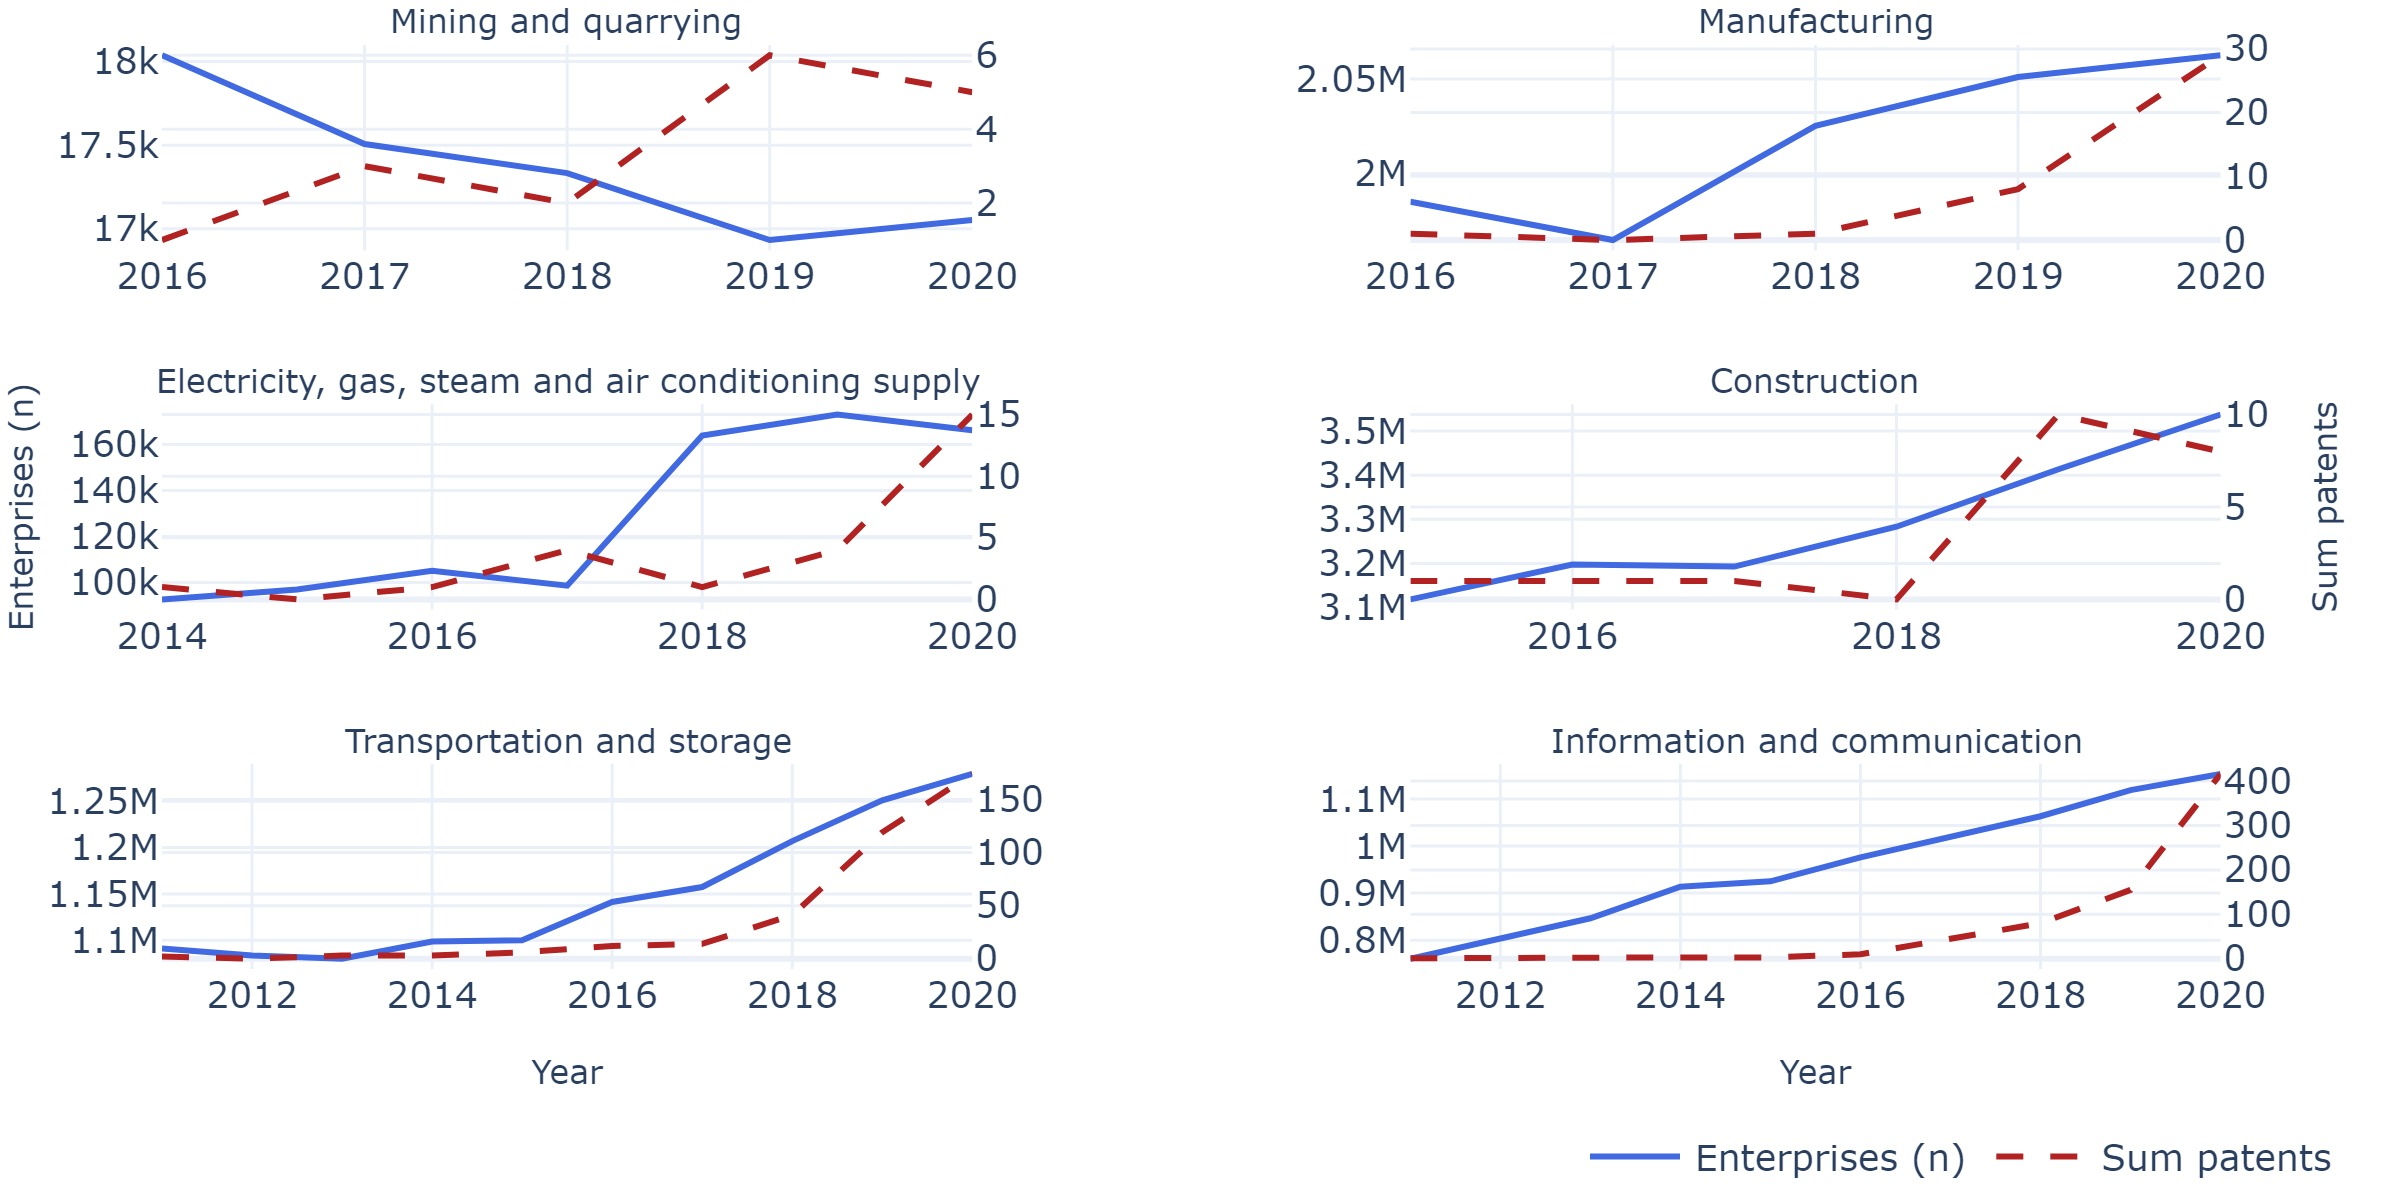
\includegraphics{rieg2023_files/figure-pdf/fig-untransformed-data-enterprises-output-1.jpeg}

}

\caption{\label{fig-untransformed-data-enterprises}Untransformed data
across all industries and NACE code `Enterprises (n)' plotted over
years}

\end{figure}

\begin{figure}[H]

{\centering 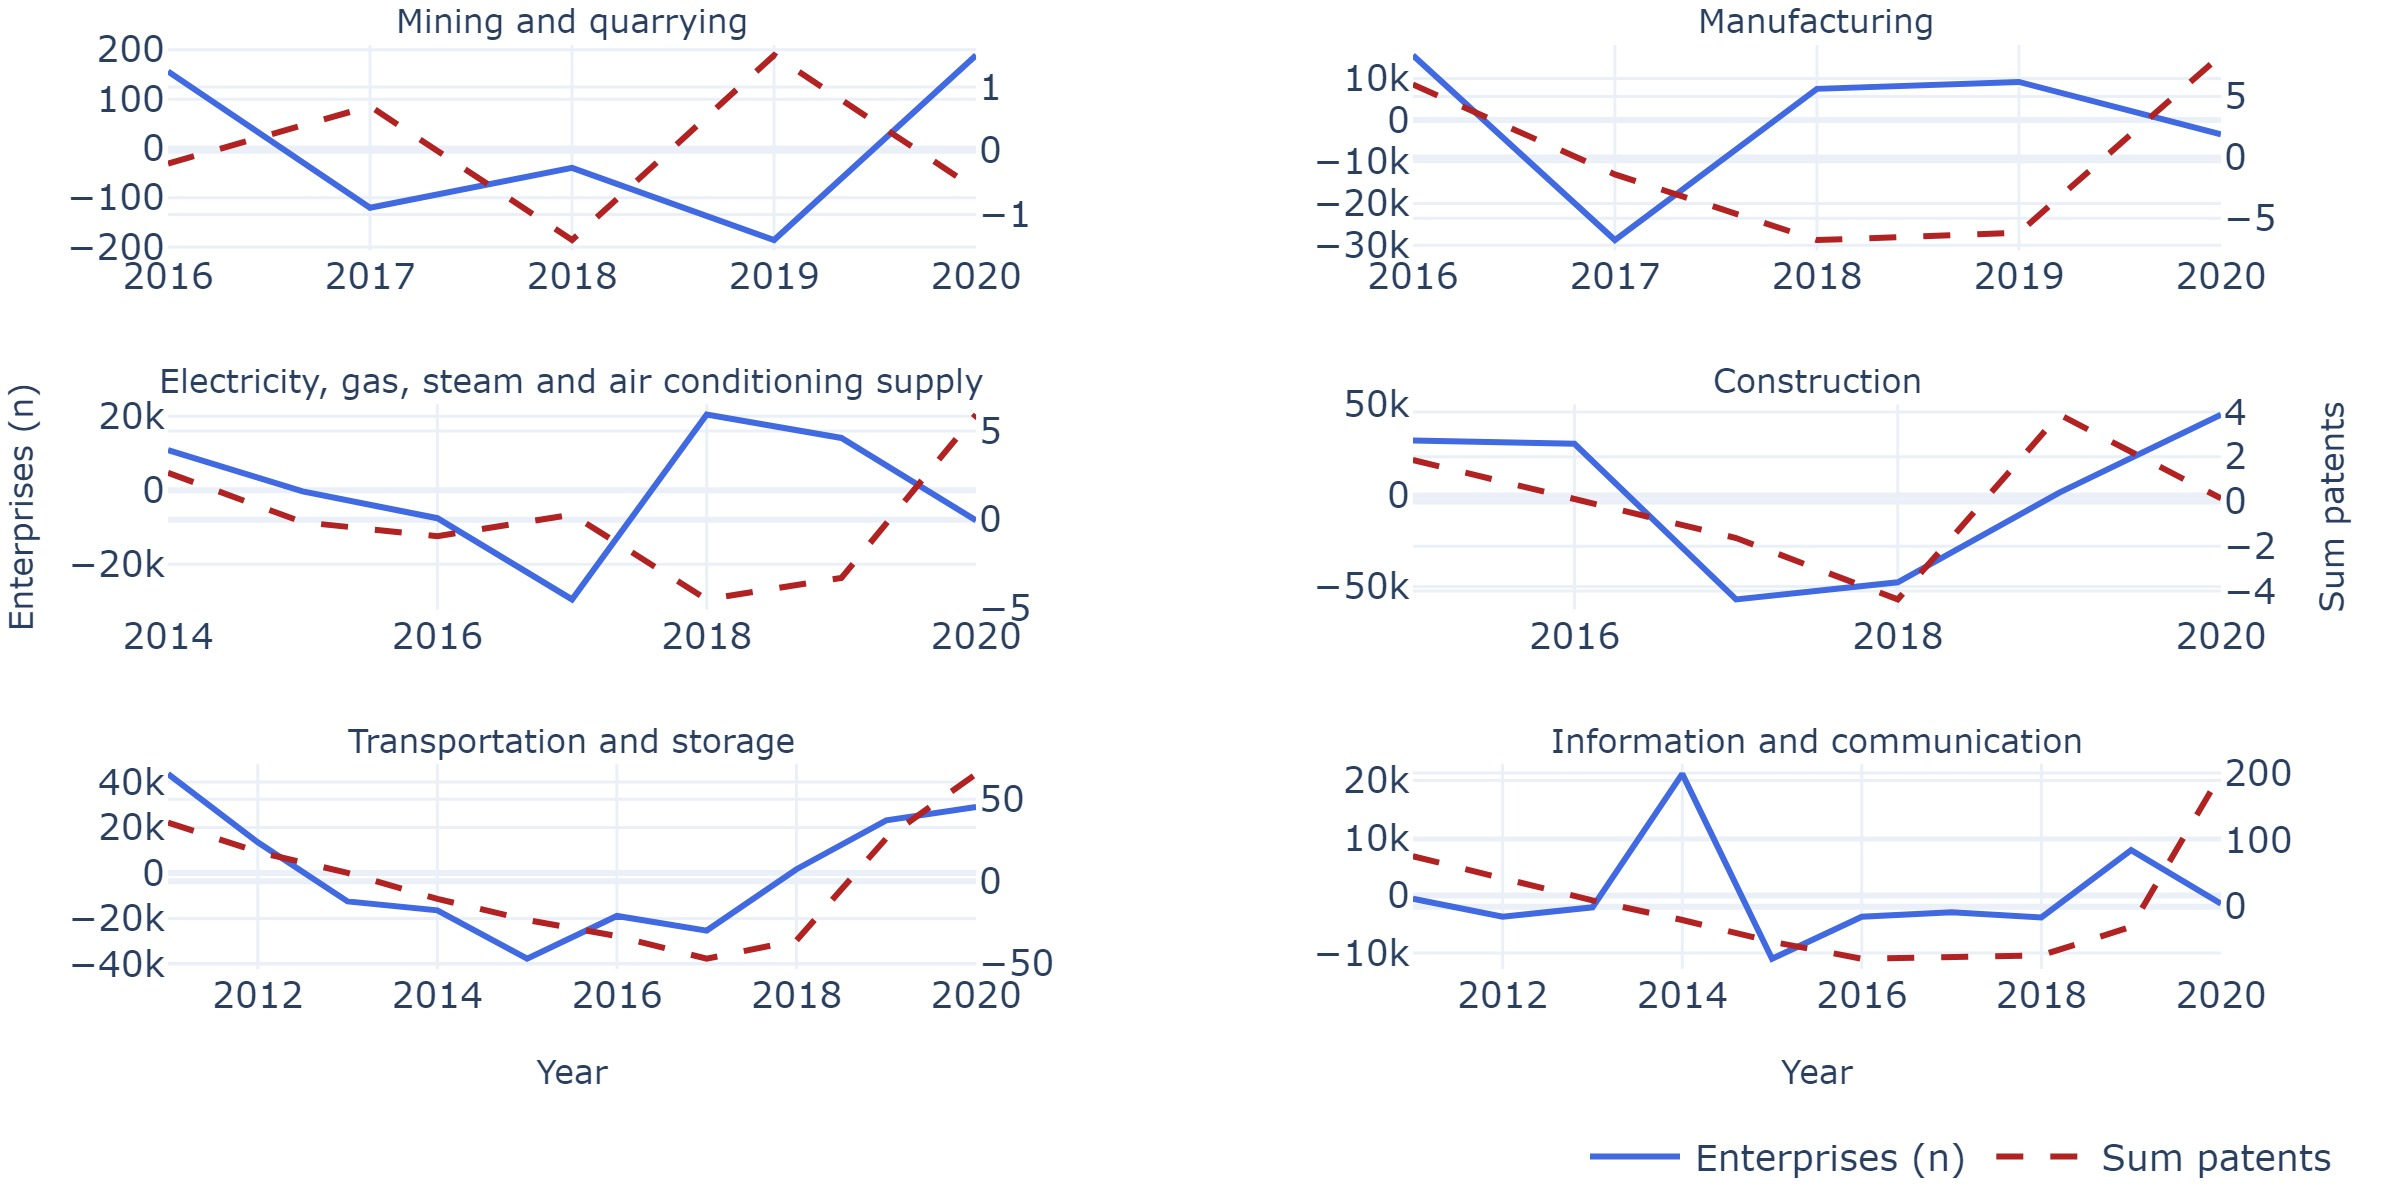
\includegraphics{rieg2023_files/figure-pdf/fig-transformed-data-example-enterprises-output-1.jpeg}

}

\caption{\label{fig-transformed-data-example-enterprises}Transformed
data across all industries and NACE code `Enterprises (n)' plotted over
years}

\end{figure}

\begin{figure}[H]

{\centering 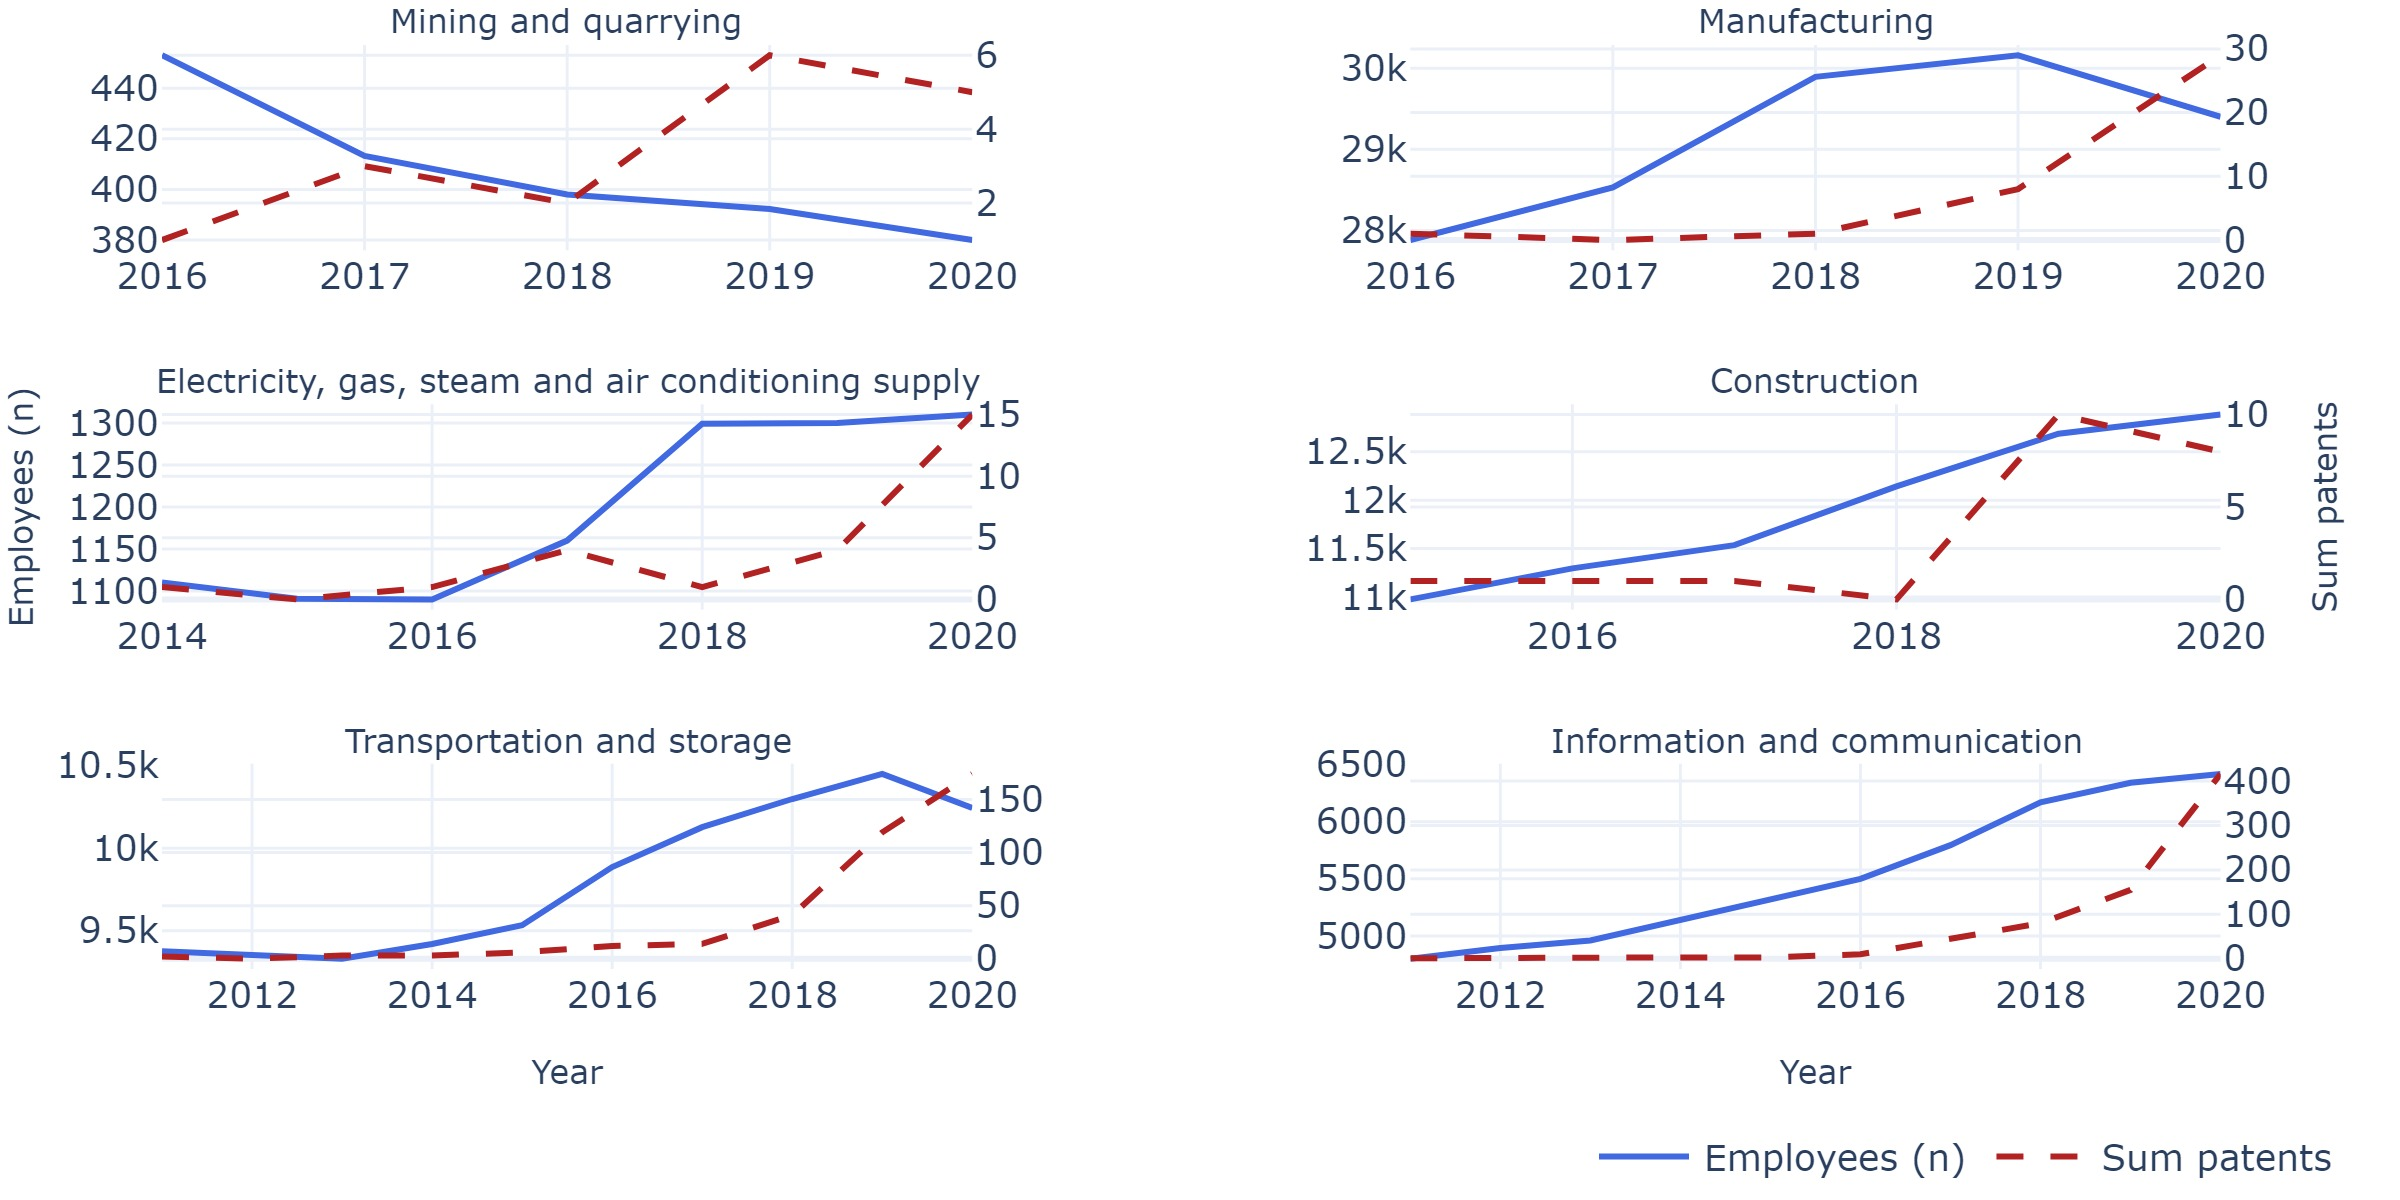
\includegraphics{rieg2023_files/figure-pdf/fig-untransformed-data-employees-output-1.jpeg}

}

\caption{\label{fig-untransformed-data-employees}Untransformed data
across all industries and NACE code `Employees (n)' plotted over years}

\end{figure}

\begin{figure}[H]

{\centering 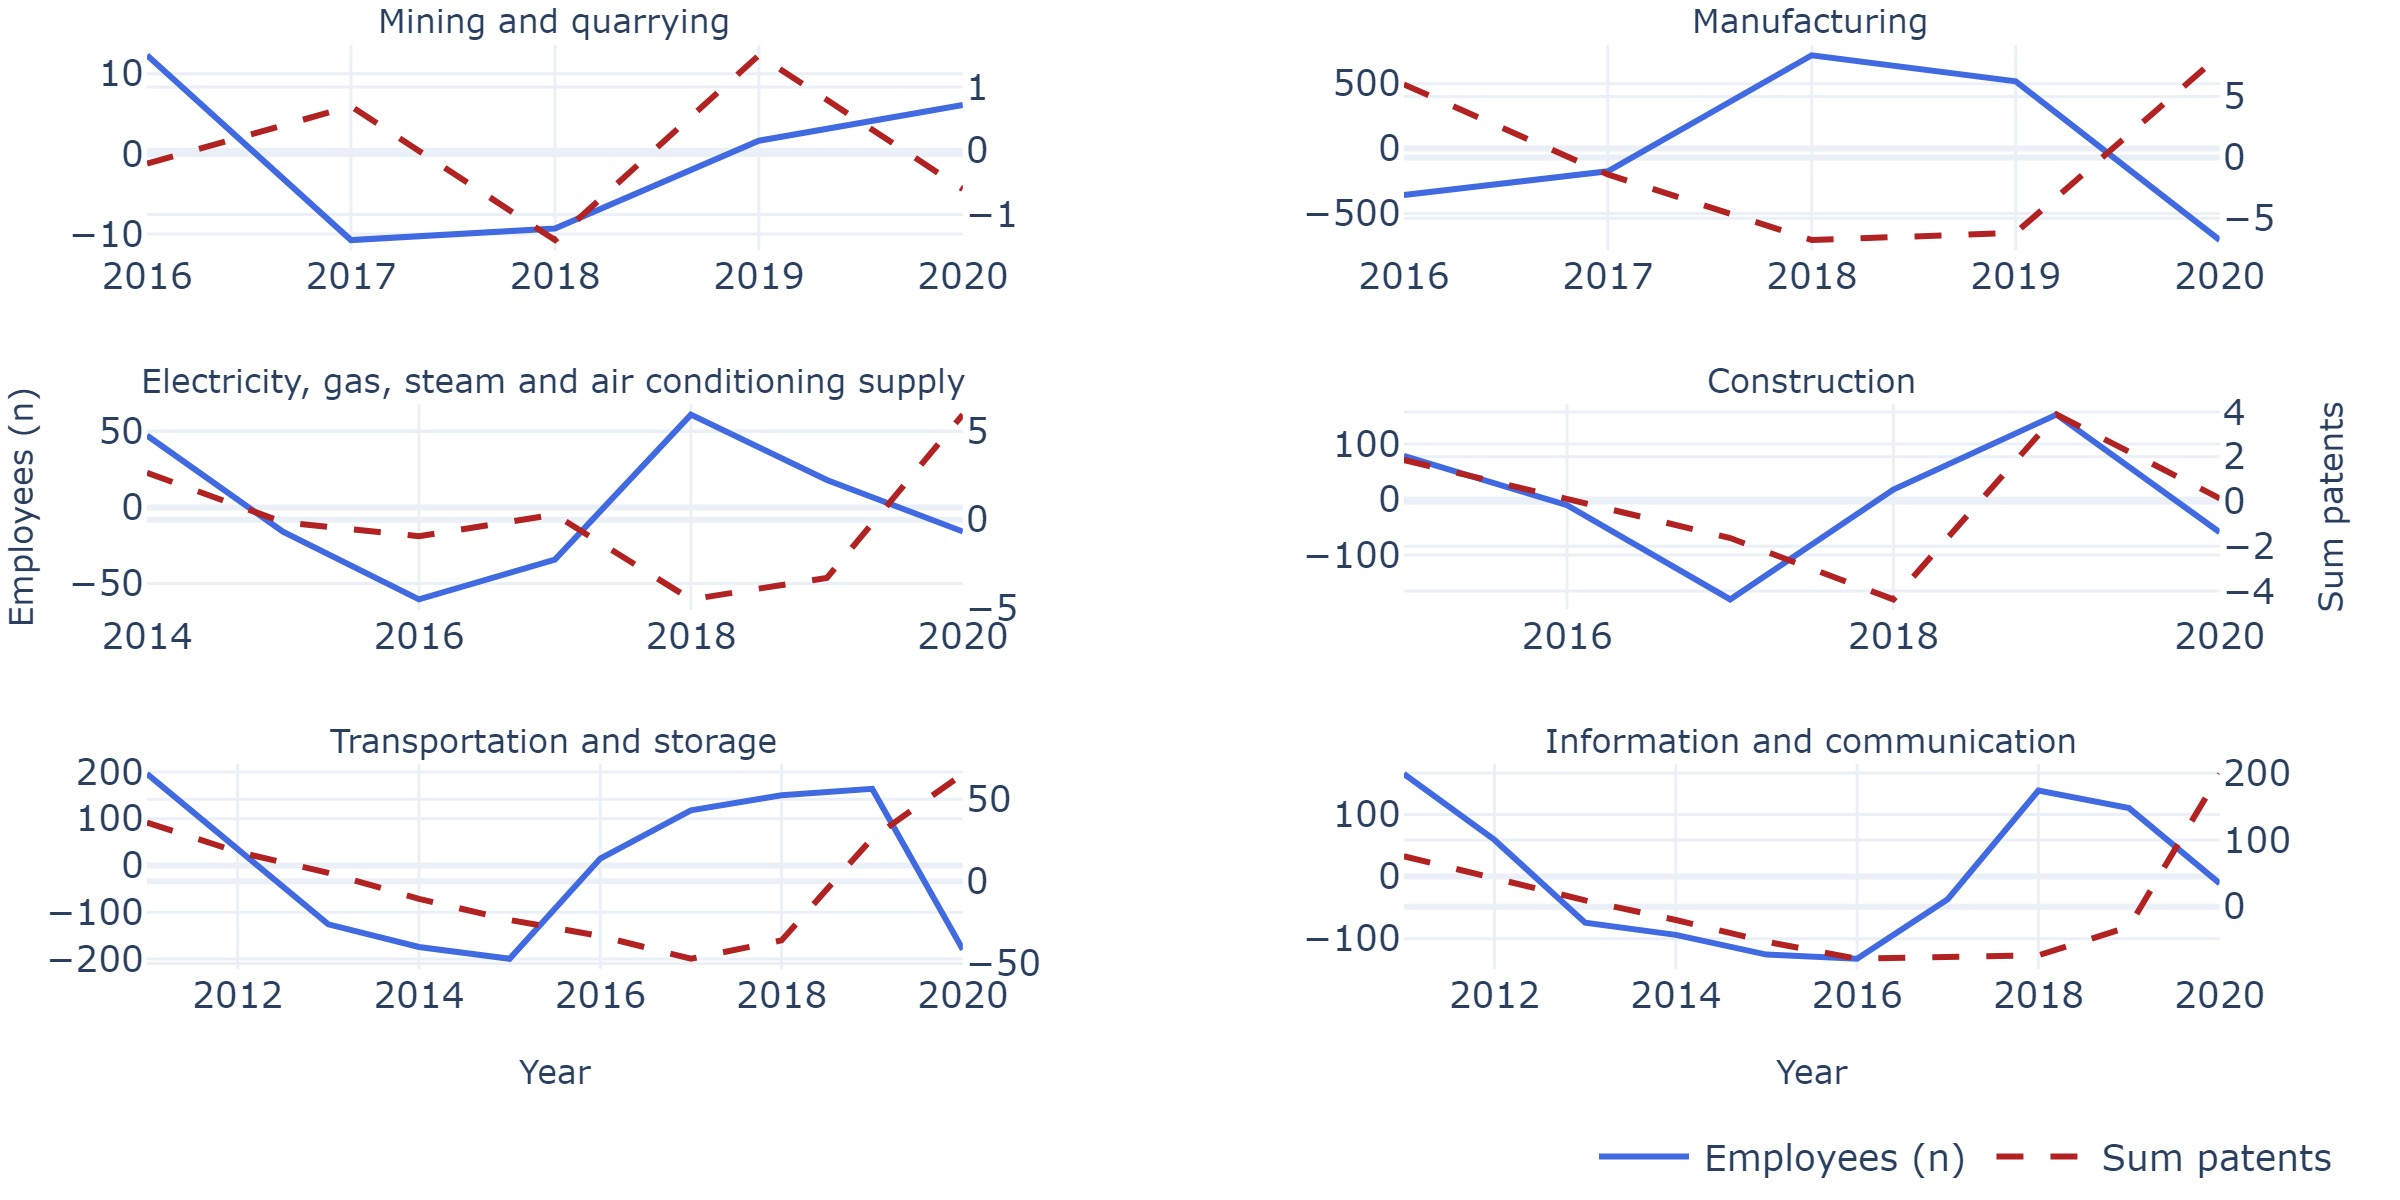
\includegraphics{rieg2023_files/figure-pdf/fig-transformed-data-employees-output-1.jpeg}

}

\caption{\label{fig-transformed-data-employees}Transformed data across
all industries and NACE code `Employees(n)' plotted over years}

\end{figure}

\begin{figure}[H]

{\centering 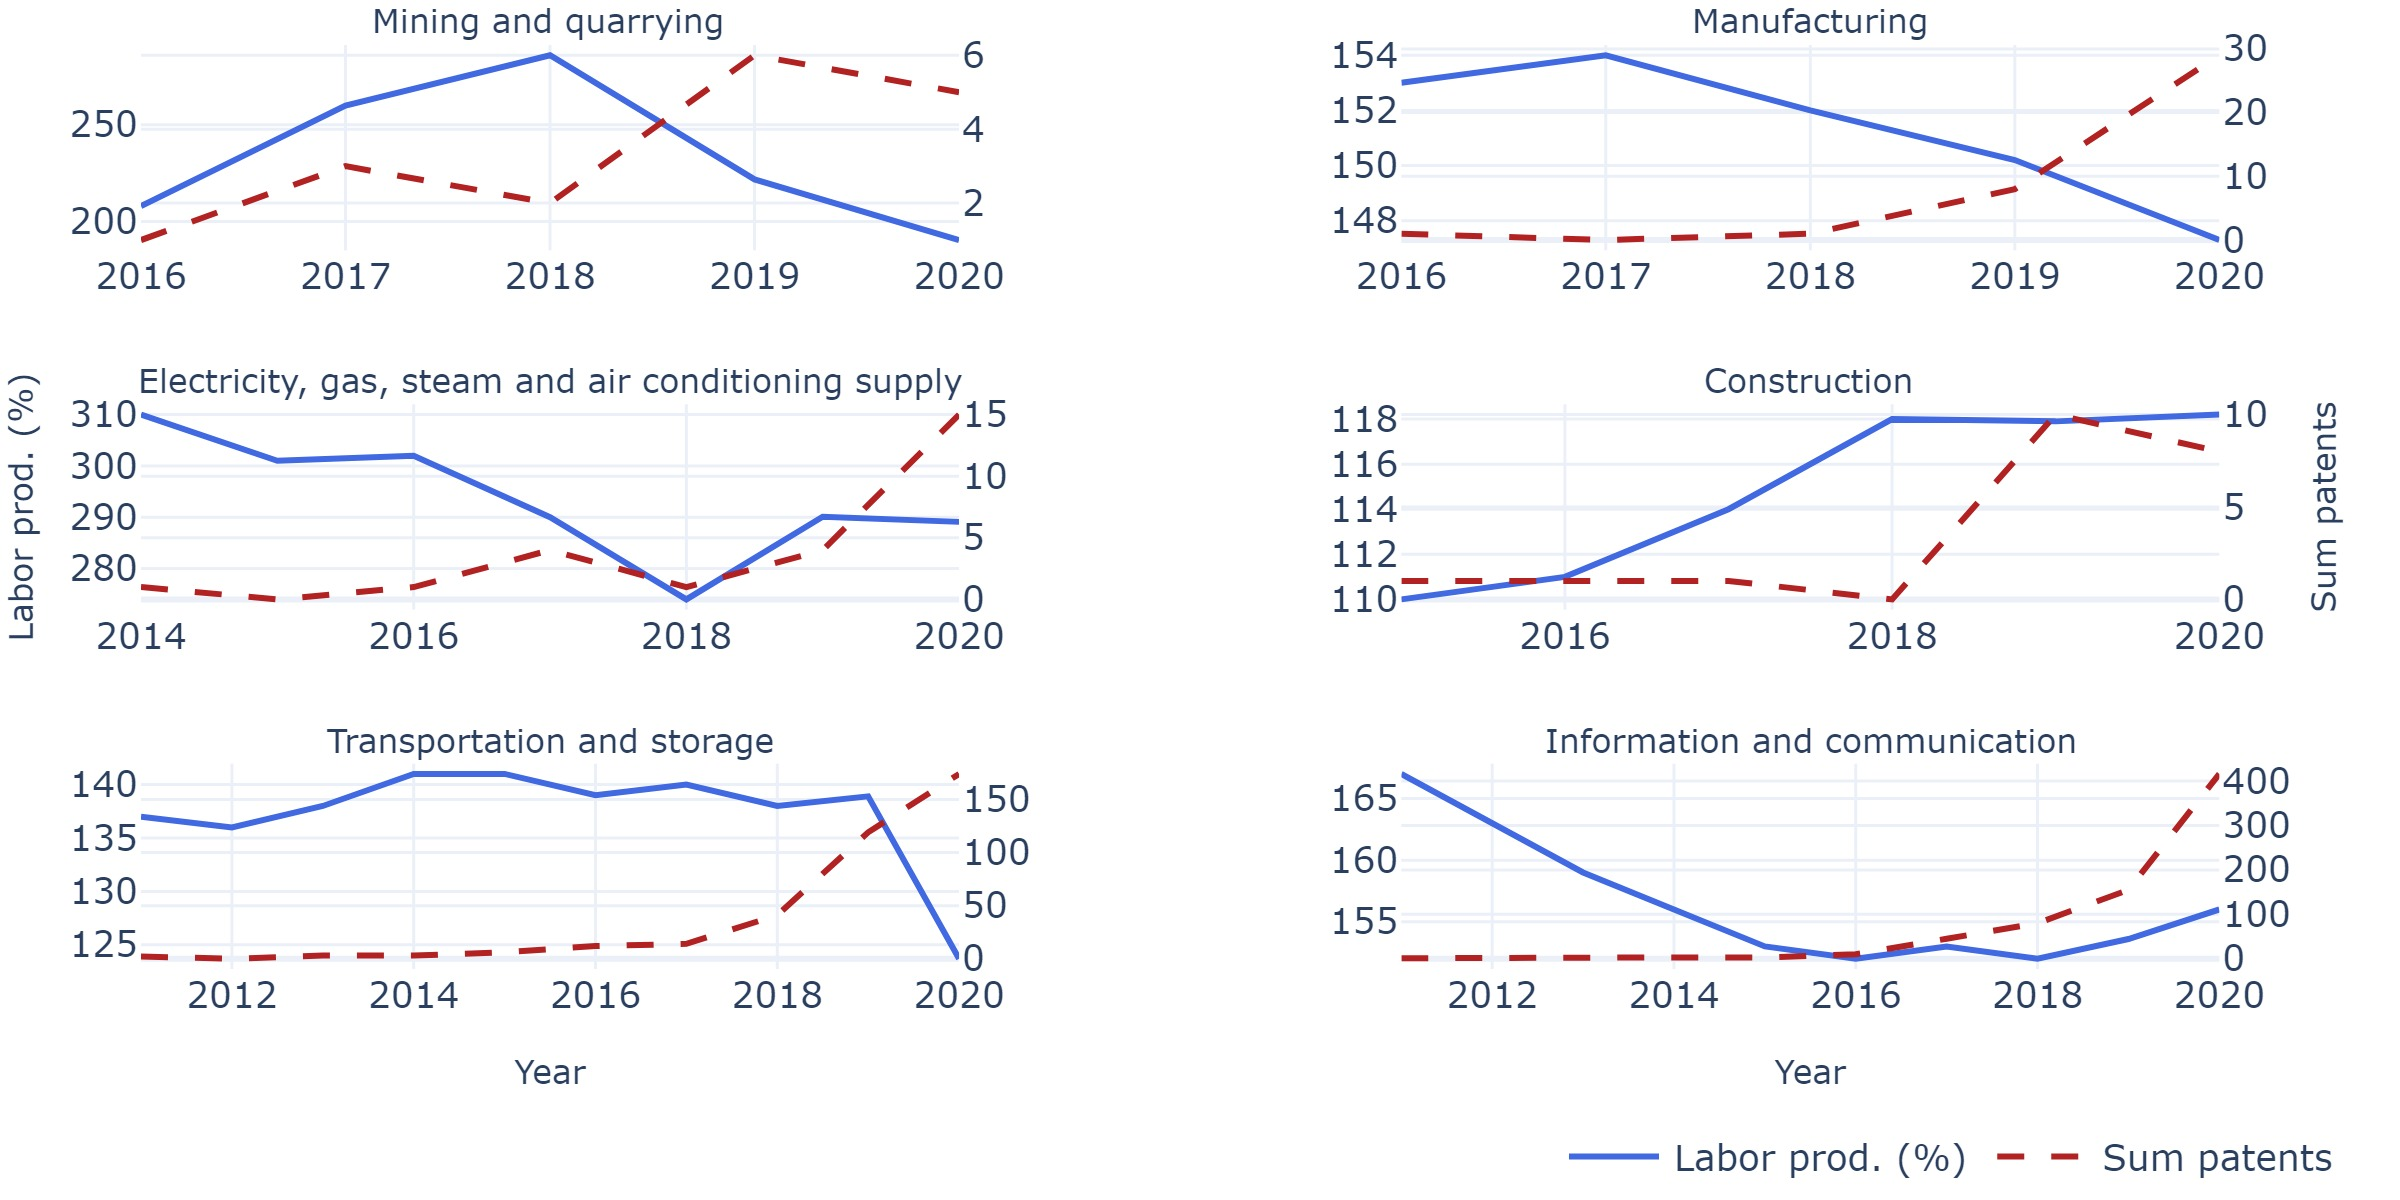
\includegraphics{rieg2023_files/figure-pdf/fig-untransformed-data-labor-prod-output-1.jpeg}

}

\caption{\label{fig-untransformed-data-labor-prod}Untransformed data
across all industries and NACE code `Wage adjusted labor productivity
(\%)' plotted over years}

\end{figure}

\begin{figure}[H]

{\centering 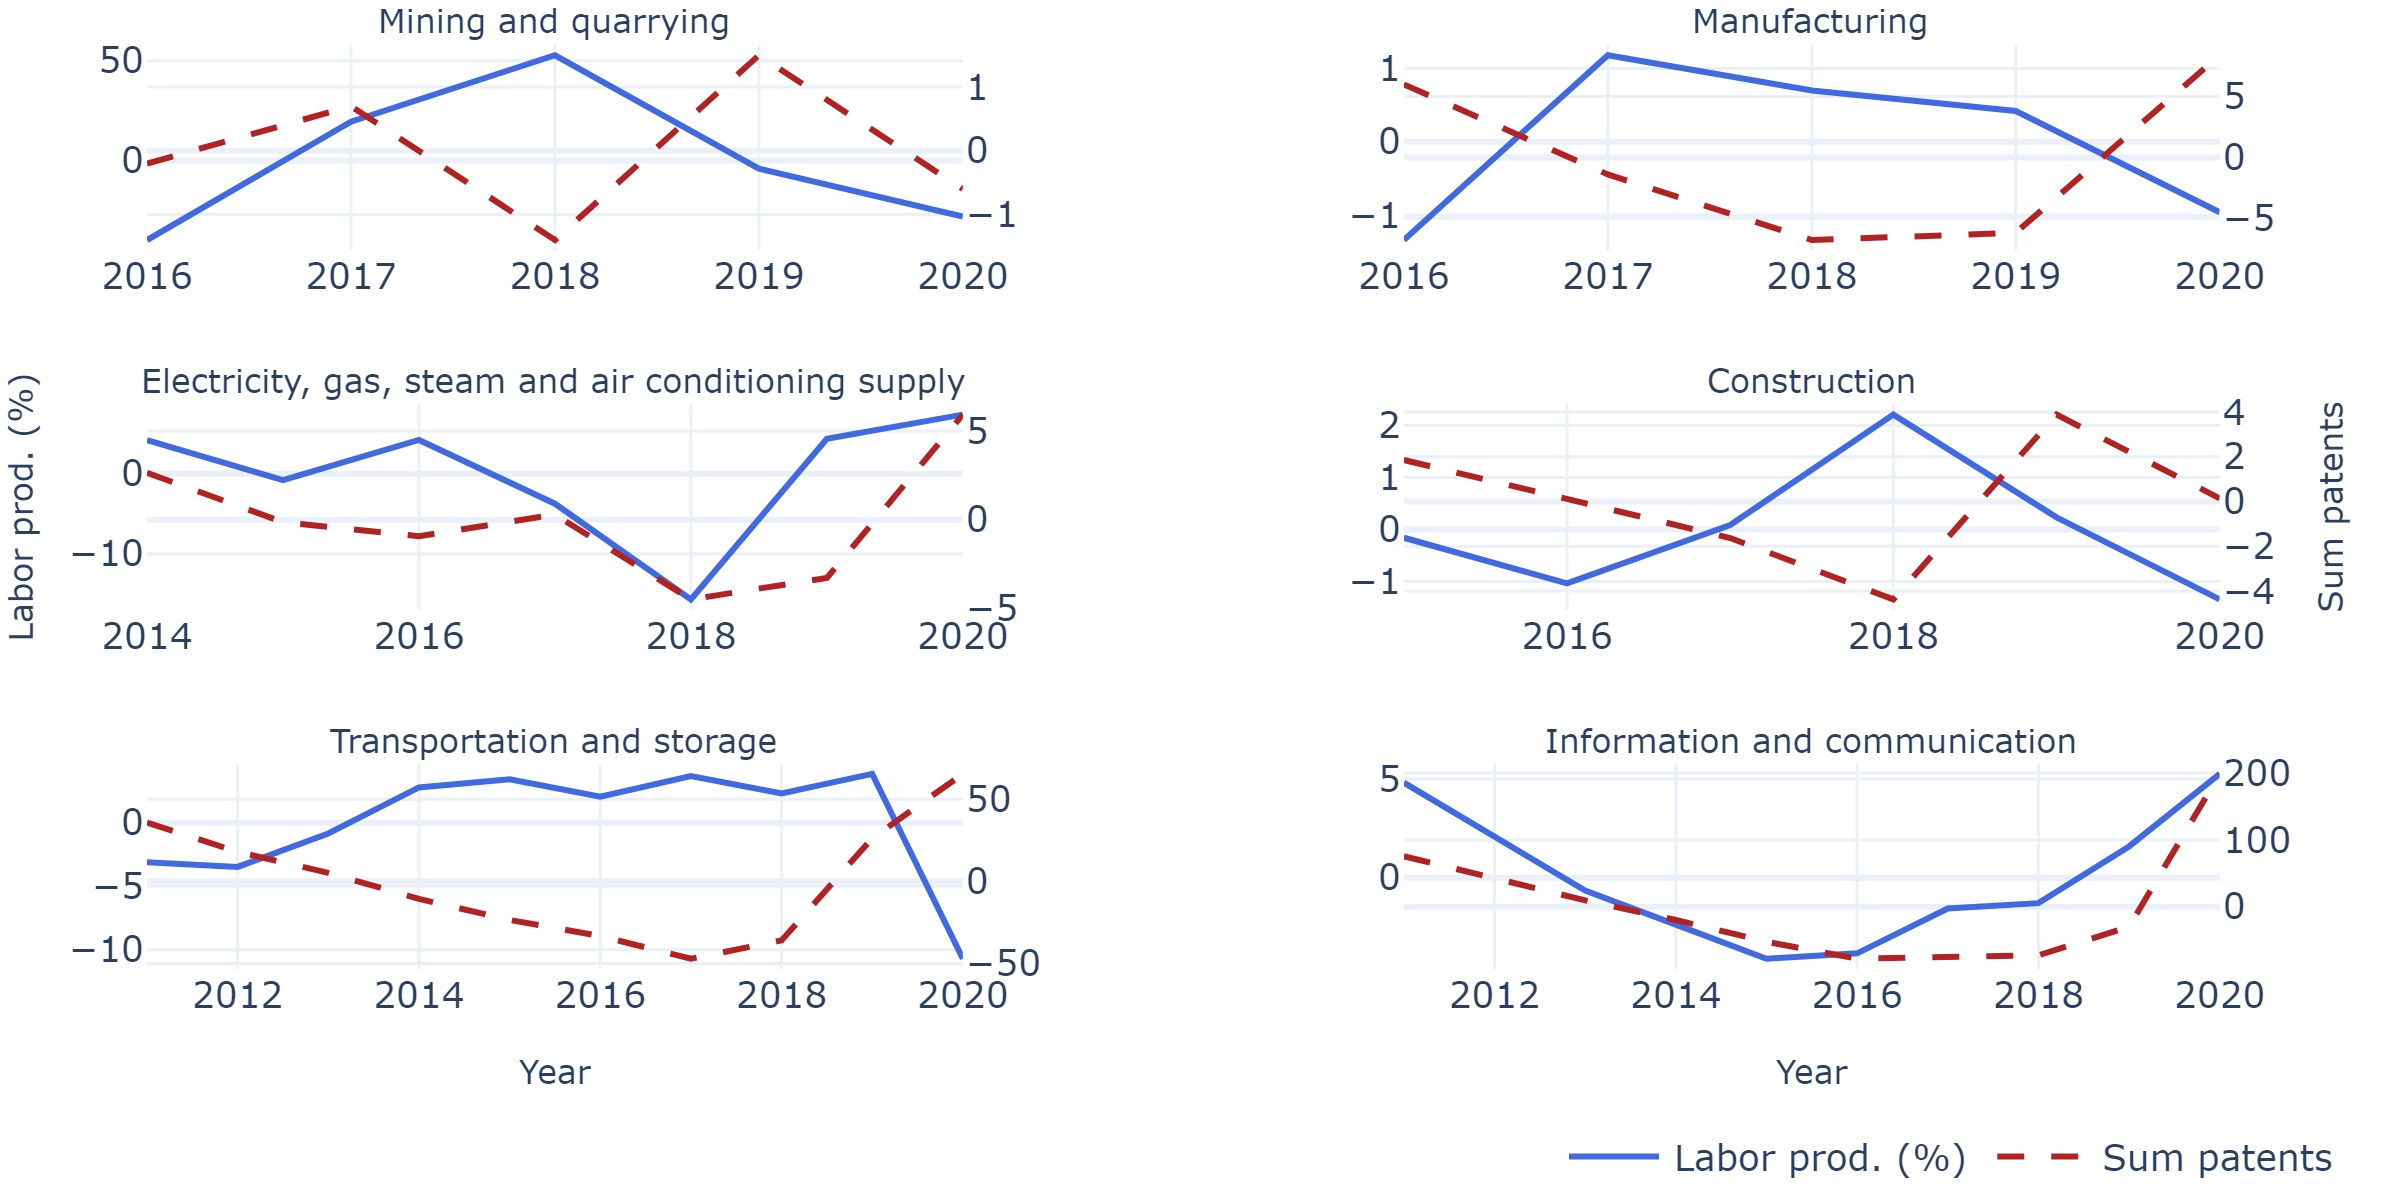
\includegraphics{rieg2023_files/figure-pdf/fig-transformed-data-labor-prod-output-1.jpeg}

}

\caption{\label{fig-transformed-data-labor-prod}Transformed data across
all industries and NACE code `Wage adjusted labor productivity (\%)'
plotted over years}

\end{figure}

\begin{figure}[H]

{\centering 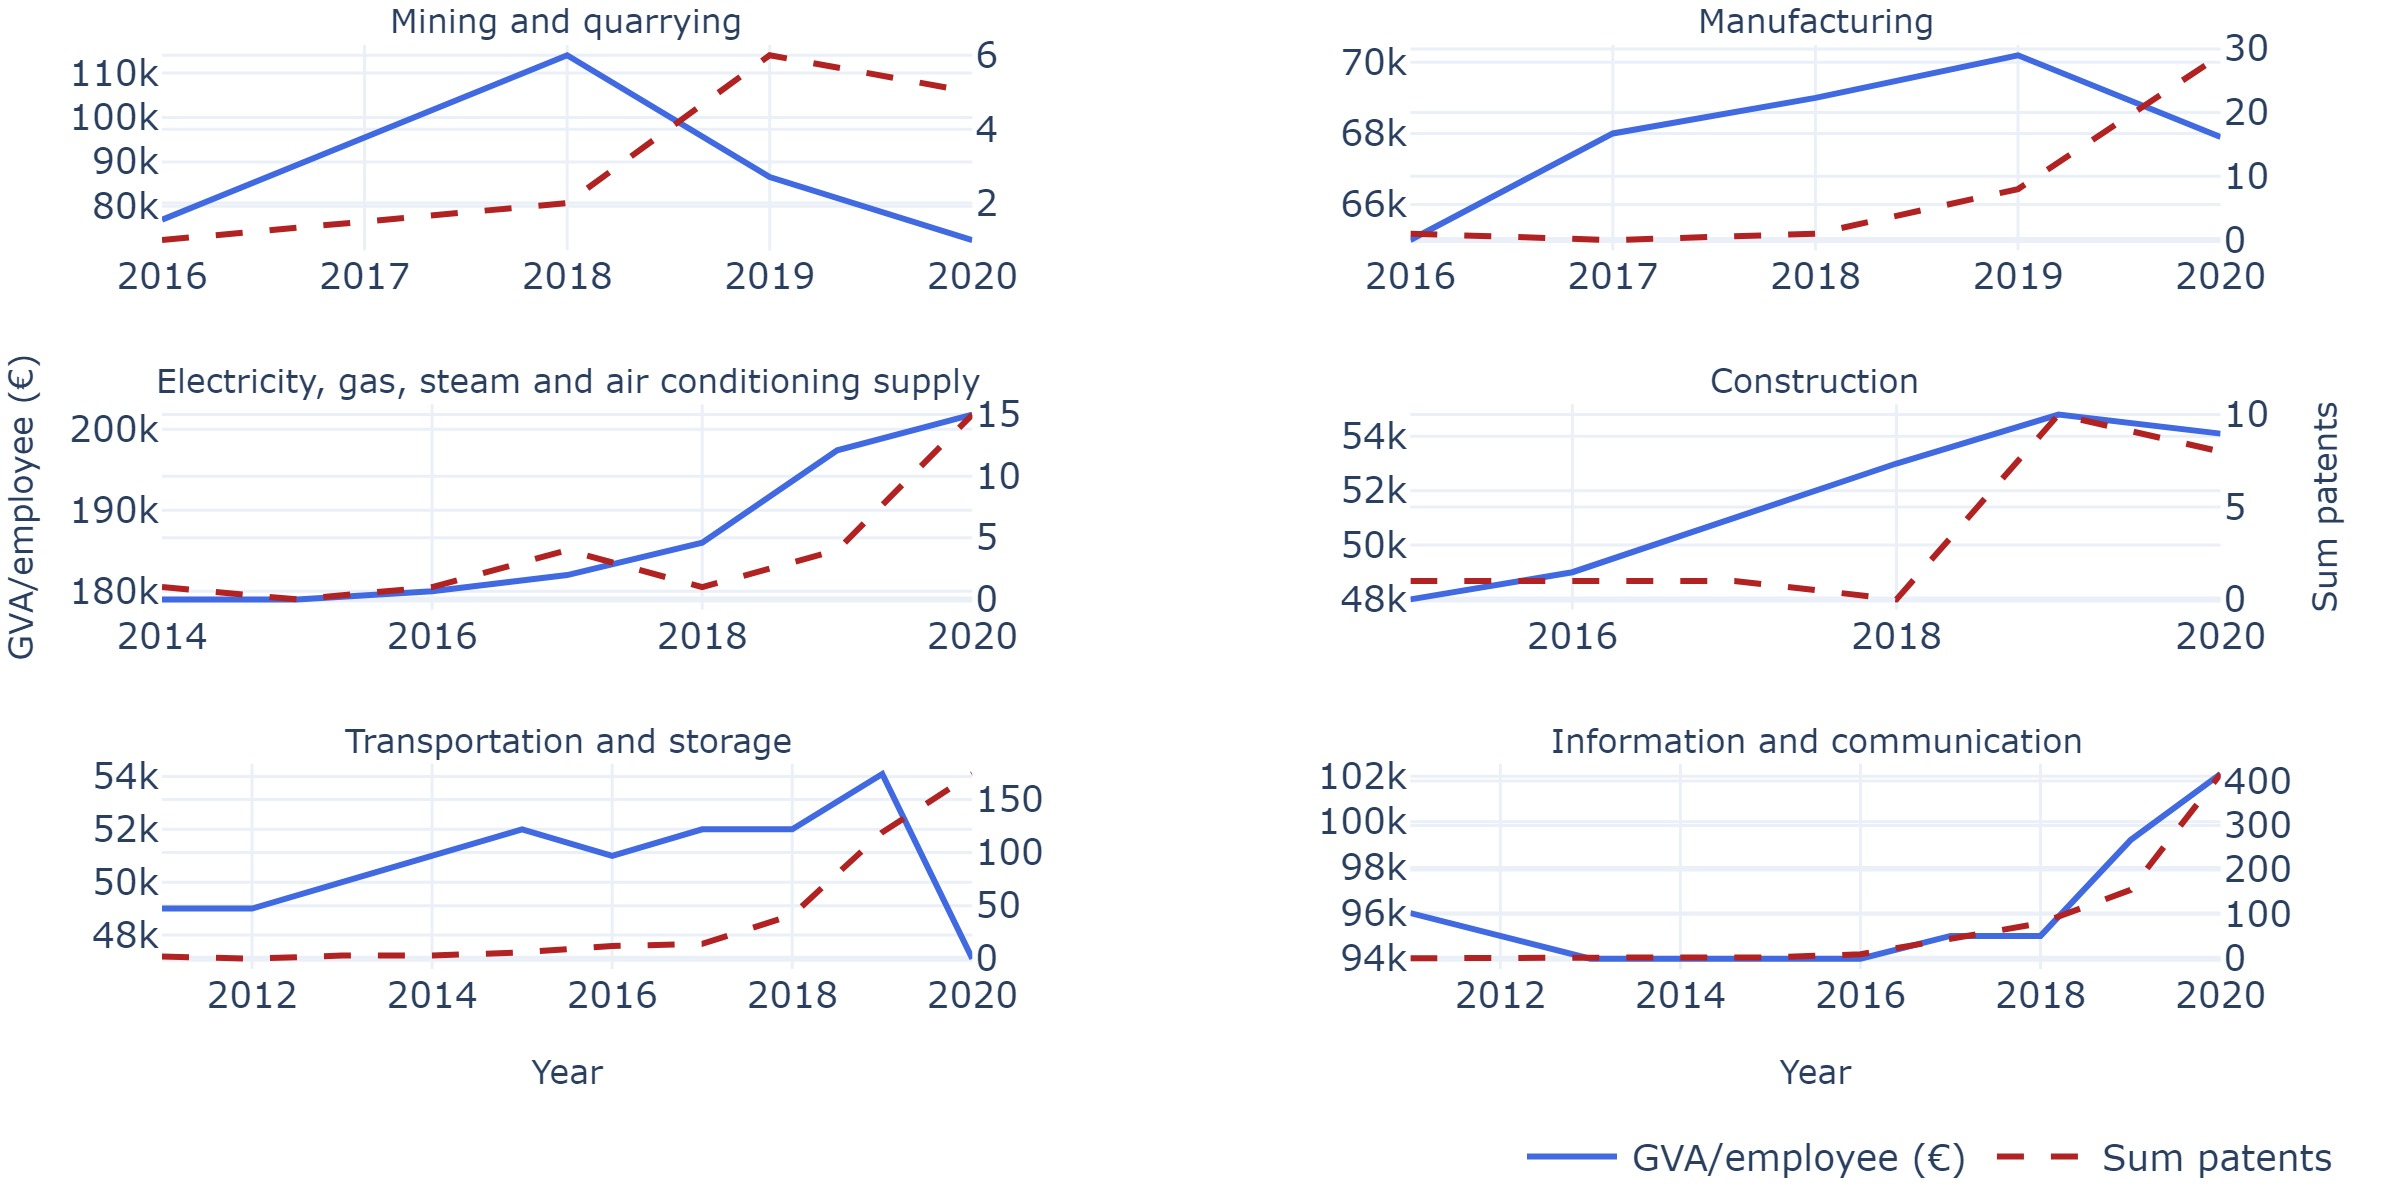
\includegraphics{rieg2023_files/figure-pdf/fig-untransformed-data-value-added-output-1.jpeg}

}

\caption{\label{fig-untransformed-data-value-added}Untransformed data
across all industries and NACE code `Gross value added per employee (€)'
plotted over years}

\end{figure}

\begin{figure}[H]

{\centering 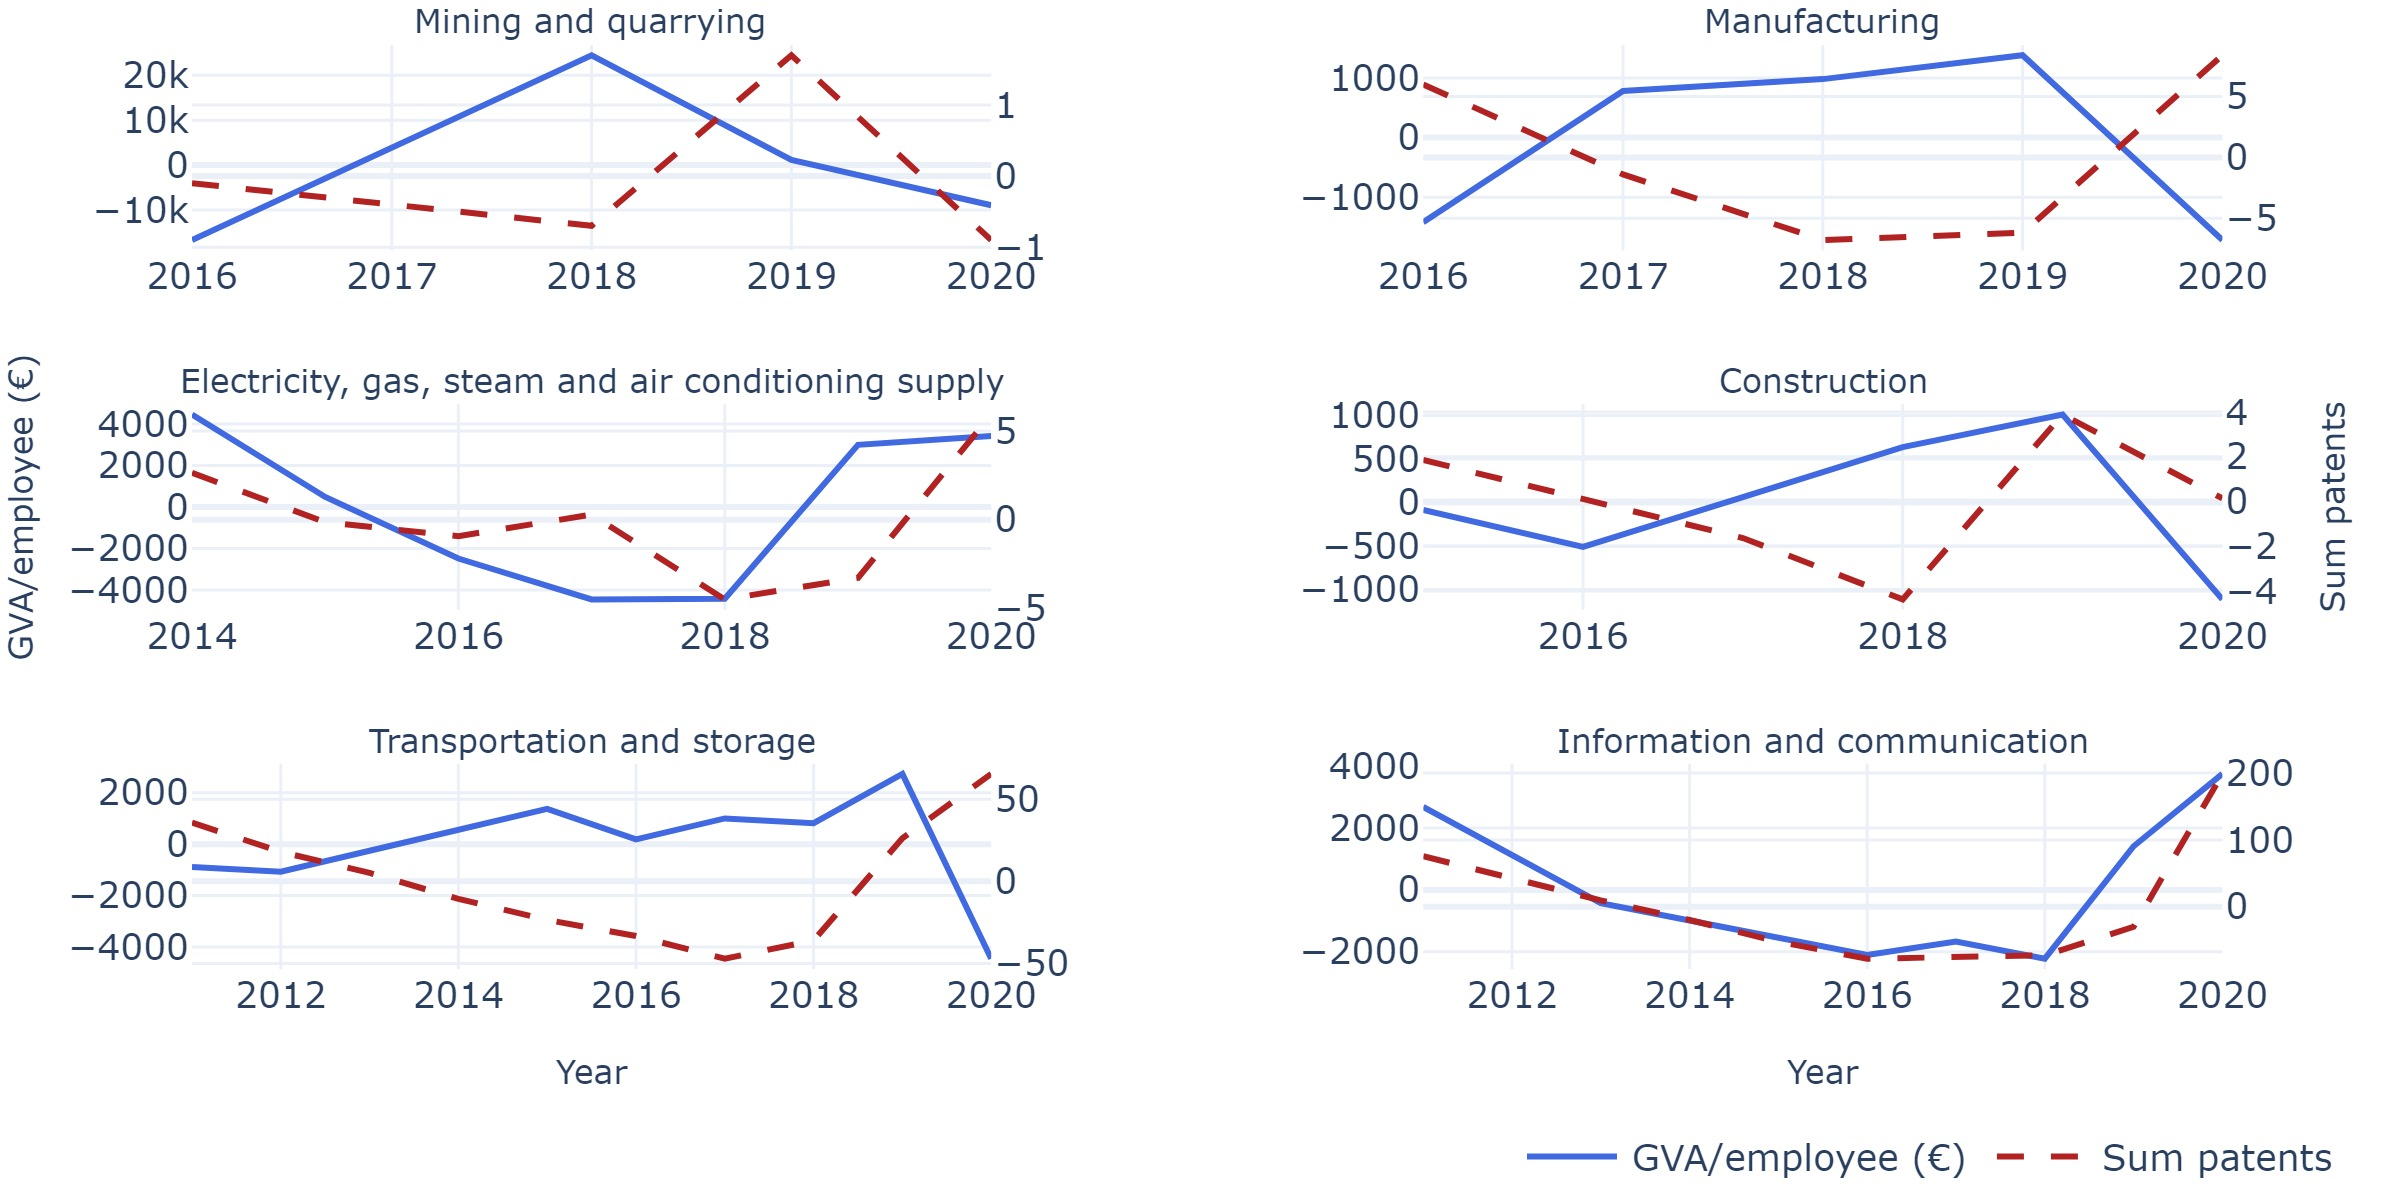
\includegraphics{rieg2023_files/figure-pdf/fig-transformed-data-value-added-output-1.jpeg}

}

\caption{\label{fig-transformed-data-value-added}Transformed data across
all industries and NACE code `Gross value added per employee (€)'
plotted over years}

\end{figure}

\begin{figure}[H]

{\centering 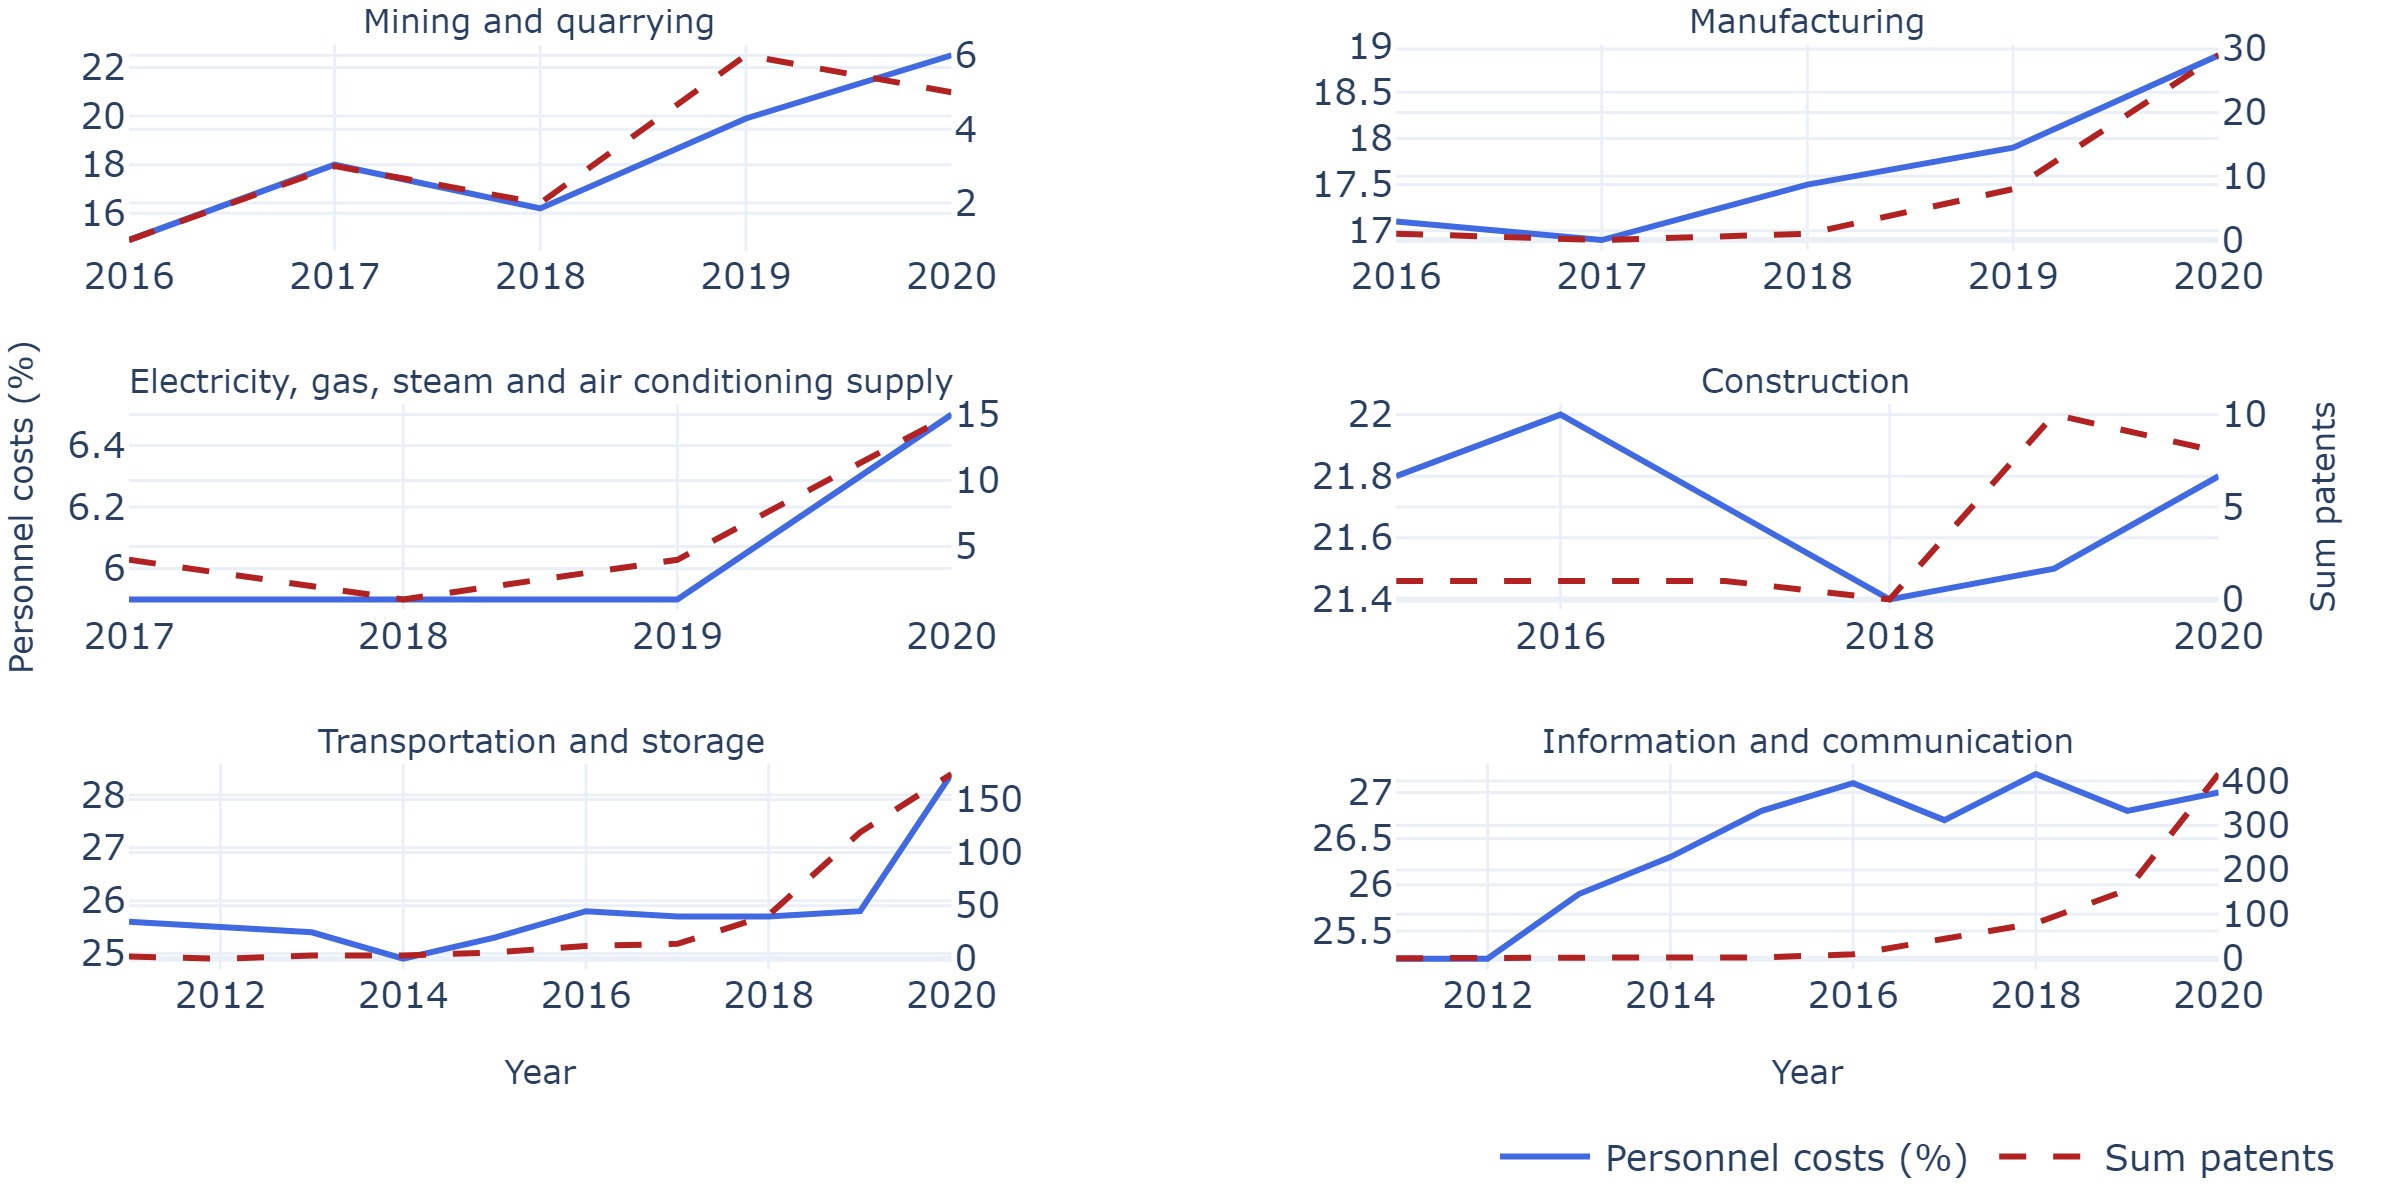
\includegraphics{rieg2023_files/figure-pdf/fig-untransformed-data-personnel-costs-output-1.jpeg}

}

\caption{\label{fig-untransformed-data-personnel-costs}Untransformed
data across all industries and NACE code `Personnel costs in production
(\%)' plotted over years}

\end{figure}

\begin{figure}[H]

{\centering 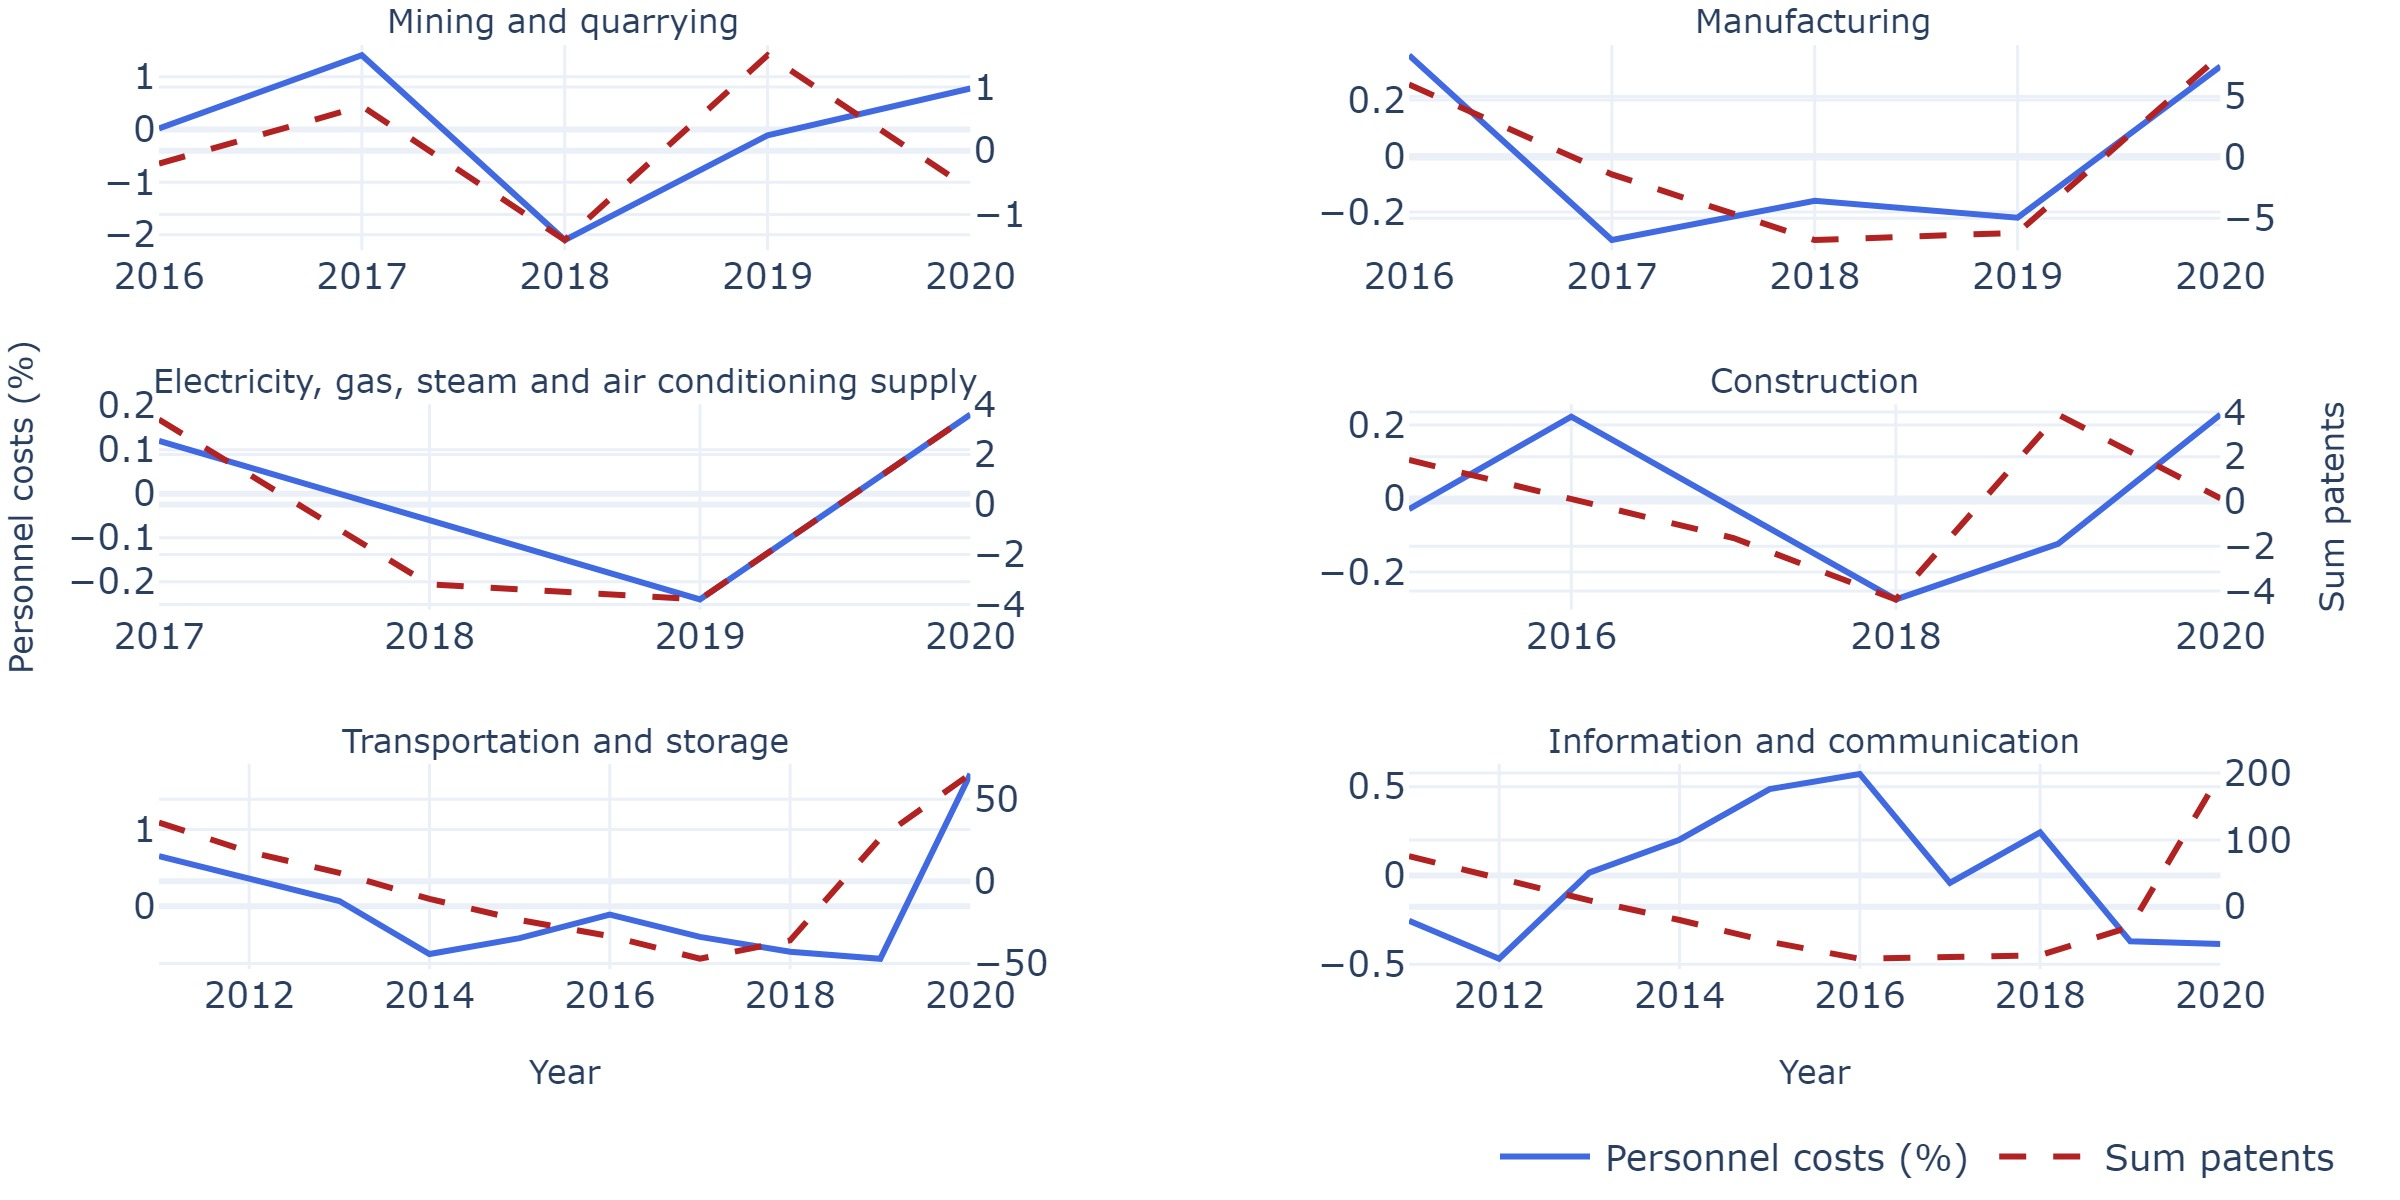
\includegraphics{rieg2023_files/figure-pdf/fig-transformed-data-personnel-costs-output-1.jpeg}

}

\caption{\label{fig-transformed-data-personnel-costs}Transformed data
across all industries and NACE code `Personnel costs in production (\%)'
plotted over years}

\end{figure}

\phantomsection\label{tbl-summary-reg-results-b}
\begin{longtable}[]{@{}
  >{\raggedright\arraybackslash}p{(\columnwidth - 10\tabcolsep) * \real{0.2033}}
  >{\raggedleft\arraybackslash}p{(\columnwidth - 10\tabcolsep) * \real{0.1545}}
  >{\raggedleft\arraybackslash}p{(\columnwidth - 10\tabcolsep) * \real{0.1382}}
  >{\raggedleft\arraybackslash}p{(\columnwidth - 10\tabcolsep) * \real{0.1545}}
  >{\raggedleft\arraybackslash}p{(\columnwidth - 10\tabcolsep) * \real{0.1626}}
  >{\raggedleft\arraybackslash}p{(\columnwidth - 10\tabcolsep) * \real{0.1870}}@{}}
\caption{\label{tbl-summary-reg-results-b}Summary of key regression
figures and tests - Mining and Quarrying (B)}\tabularnewline
\toprule\noalign{}
\begin{minipage}[b]{\linewidth}\raggedright
\end{minipage} & \begin{minipage}[b]{\linewidth}\raggedleft
Enterprises (n)
\end{minipage} & \begin{minipage}[b]{\linewidth}\raggedleft
Employees (n)
\end{minipage} & \begin{minipage}[b]{\linewidth}\raggedleft
Labor prod. (\%)
\end{minipage} & \begin{minipage}[b]{\linewidth}\raggedleft
GVA/employee (€)
\end{minipage} & \begin{minipage}[b]{\linewidth}\raggedleft
Personnel costs (\%)
\end{minipage} \\
\midrule\noalign{}
\endfirsthead
\toprule\noalign{}
\begin{minipage}[b]{\linewidth}\raggedright
\end{minipage} & \begin{minipage}[b]{\linewidth}\raggedleft
Enterprises (n)
\end{minipage} & \begin{minipage}[b]{\linewidth}\raggedleft
Employees (n)
\end{minipage} & \begin{minipage}[b]{\linewidth}\raggedleft
Labor prod. (\%)
\end{minipage} & \begin{minipage}[b]{\linewidth}\raggedleft
GVA/employee (€)
\end{minipage} & \begin{minipage}[b]{\linewidth}\raggedleft
Personnel costs (\%)
\end{minipage} \\
\midrule\noalign{}
\endhead
\bottomrule\noalign{}
\endlastfoot
F-statistic & 0.568 & 0.002 & 0.065 & 0.021 & 0.433 \\
Prob (F-statistic) & 0.638 & 0.998 & 0.939 & 0.979 & 0.698 \\
Observations & 5 & 5 & 5 & 4 & 5 \\
R-squared & 0.362 & 0.002 & 0.061 & 0.041 & 0.302 \\
Adj. R-squared & -0.275 & -0.997 & -0.878 & -1.877 & -0.395 \\
Jarque-Bera & 0.778 & 0.786 & 0.754 & 0.768 & 0.73 \\
Skew & 0.053 & 0.039 & -0.122 & 0.677 & -0.102 \\
Kurtosis & 1.45 & 1.481 & 1.373 & 1.846 & 1.272 \\
Durbin-Watson & 1.384 & 1.723 & 1.437 & 2.239 & 2.114 \\
Breusch-Pagan & 0.1 & 0.11 & 0.093 & 0.399 & 0.181 \\
Sum patents Coef. & 0.398 & 0.959 & 0.753 & 0.942 & 0.45 \\
Sum patents p value & 0.398 & 0.959 & 0.753 & 0.942 & 0.45 \\
Sum patents SE & 83.139 & 6.204 & 22.635 & 14778.9 & 0.693 \\
Sum patents Conf. lower & -446.364 & -26.329 & -105.535 & -189125 &
-2.336 \\
Sum patents Conf. upper & 269.07 & 27.055 & 89.245 & 186443 & 3.626 \\
Year Coef. & 1 & 1 & 1 & 0.882 & 1 \\
Year p value & 1 & 1 & 1 & 0.882 & 1 \\
Year SE & 59.373 & 4.43 & 16.164 & 10239.1 & 0.495 \\
Year Conf. lower & -255.461 & -19.062 & -69.55 & -128179 & -2.129 \\
Year Conf. upper & 255.461 & 19.062 & 69.55 & 132022 & 2.129 \\
\end{longtable}

\vspace{-1.5em}\setstretch{1}\begin{flushleft}\footnotesize\textit{Jarque-Bera test for normality of residuals, p value < 0.05 indicates non-normality; Durbin-Watson test for autocorrelation, values between 1.5 and 2.5 indicate no autocorrelation; Breusch-Pagan test for heteroskedasticity, p value < 0.05 indicates heteroskedasticity; Coef. = Coefficient; Conf. lower = lower bound of 0.95 confidence interval, conf. upper = upper bound of 0.95 confidence interval; SE = standard error.}\end{flushleft}\setstretch{1.5}

\phantomsection\label{tbl-summary-reg-results-c}
\begin{longtable}[]{@{}
  >{\raggedright\arraybackslash}p{(\columnwidth - 10\tabcolsep) * \real{0.2033}}
  >{\raggedleft\arraybackslash}p{(\columnwidth - 10\tabcolsep) * \real{0.1545}}
  >{\raggedleft\arraybackslash}p{(\columnwidth - 10\tabcolsep) * \real{0.1382}}
  >{\raggedleft\arraybackslash}p{(\columnwidth - 10\tabcolsep) * \real{0.1545}}
  >{\raggedleft\arraybackslash}p{(\columnwidth - 10\tabcolsep) * \real{0.1626}}
  >{\raggedleft\arraybackslash}p{(\columnwidth - 10\tabcolsep) * \real{0.1870}}@{}}
\caption{\label{tbl-summary-reg-results-c}Summary table of regression
figures and tests - Manufacturing (C)}\tabularnewline
\toprule\noalign{}
\begin{minipage}[b]{\linewidth}\raggedright
\end{minipage} & \begin{minipage}[b]{\linewidth}\raggedleft
Enterprises (n)
\end{minipage} & \begin{minipage}[b]{\linewidth}\raggedleft
Employees (n)
\end{minipage} & \begin{minipage}[b]{\linewidth}\raggedleft
Labor prod. (\%)
\end{minipage} & \begin{minipage}[b]{\linewidth}\raggedleft
GVA/employee (€)
\end{minipage} & \begin{minipage}[b]{\linewidth}\raggedleft
Personnel costs (\%)
\end{minipage} \\
\midrule\noalign{}
\endfirsthead
\toprule\noalign{}
\begin{minipage}[b]{\linewidth}\raggedright
\end{minipage} & \begin{minipage}[b]{\linewidth}\raggedleft
Enterprises (n)
\end{minipage} & \begin{minipage}[b]{\linewidth}\raggedleft
Employees (n)
\end{minipage} & \begin{minipage}[b]{\linewidth}\raggedleft
Labor prod. (\%)
\end{minipage} & \begin{minipage}[b]{\linewidth}\raggedleft
GVA/employee (€)
\end{minipage} & \begin{minipage}[b]{\linewidth}\raggedleft
Personnel costs (\%)
\end{minipage} \\
\midrule\noalign{}
\endhead
\bottomrule\noalign{}
\endlastfoot
F-statistic & 0 & 10.222 & 2.163 & 17.29 & 3.525 \\
Prob (F-statistic) & 1 & 0.089 & 0.316 & 0.055 & 0.221 \\
Observations & 5 & 5 & 5 & 5 & 5 \\
R-squared & 0 & 0.911 & 0.684 & 0.945 & 0.779 \\
Adj. R-squared & -1 & 0.822 & 0.368 & 0.891 & 0.558 \\
Jarque-Bera & 0.649 & 0.706 & 0.684 & 0.867 & 0.655 \\
Skew & -0.992 & -0.873 & 0.912 & 0.356 & -0.983 \\
Kurtosis & 2.538 & 2.456 & 2.443 & 2.069 & 2.555 \\
Durbin-Watson & 2.816 & 3.173 & 2.738 & 3.42 & 3.065 \\
Breusch-Pagan & 0.445 & 0.427 & 0.453 & 0.367 & 0.433 \\
Sum patents Coef. & 0.994 & 0.046 & 0.173 & 0.028 & 0.117 \\
Sum patents p value & 0.994 & 0.046 & 0.173 & 0.028 & 0.117 \\
Sum patents SE & 1778.57 & 18.244 & 0.063 & 34.574 & 0.015 \\
Sum patents Conf. lower & -7667.17 & -160.985 & -0.399 & -352.071 &
-0.025 \\
Sum patents Conf. upper & 7637.95 & -3.993 & 0.139 & -54.554 & 0.105 \\
Year Coef. & 1 & 1 & 1 & 1 & 1 \\
Year p value & 1 & 1 & 1 & 1 & 1 \\
Year SE & 7817.61 & 80.189 & 0.275 & 151.967 & 0.066 \\
Year Conf. lower & -33636.5 & -345.027 & -1.182 & -653.862 & -0.285 \\
Year Conf. upper & 33636.5 & 345.027 & 1.182 & 653.862 & 0.285 \\
\end{longtable}

\vspace{-1.5em}\setstretch{1}\begin{flushleft}\footnotesize\textit{Jarque-Bera test for normality of residuals, p value < 0.05 indicates non-normality; Durbin-Watson test for autocorrelation, values between 1.5 and 2.5 indicate no autocorrelation; Breusch-Pagan test for heteroskedasticity, p value < 0.05 indicates heteroskedasticity; Coef. = Coefficient; Conf. lower = lower bound of 0.95 confidence interval, conf. upper = upper bound of 0.95 confidence interval; SE = standard error.}\end{flushleft}\setstretch{1.5}

\phantomsection\label{tbl-summary-reg-results-d}
\begin{longtable}[]{@{}
  >{\raggedright\arraybackslash}p{(\columnwidth - 10\tabcolsep) * \real{0.2033}}
  >{\raggedleft\arraybackslash}p{(\columnwidth - 10\tabcolsep) * \real{0.1545}}
  >{\raggedleft\arraybackslash}p{(\columnwidth - 10\tabcolsep) * \real{0.1382}}
  >{\raggedleft\arraybackslash}p{(\columnwidth - 10\tabcolsep) * \real{0.1545}}
  >{\raggedleft\arraybackslash}p{(\columnwidth - 10\tabcolsep) * \real{0.1626}}
  >{\raggedleft\arraybackslash}p{(\columnwidth - 10\tabcolsep) * \real{0.1870}}@{}}
\caption{\label{tbl-summary-reg-results-d}Summary of key regression
figures and tests - Electricity, gas, steam and air conditioning supply
(D)}\tabularnewline
\toprule\noalign{}
\begin{minipage}[b]{\linewidth}\raggedright
\end{minipage} & \begin{minipage}[b]{\linewidth}\raggedleft
Enterprises (n)
\end{minipage} & \begin{minipage}[b]{\linewidth}\raggedleft
Employees (n)
\end{minipage} & \begin{minipage}[b]{\linewidth}\raggedleft
Labor prod. (\%)
\end{minipage} & \begin{minipage}[b]{\linewidth}\raggedleft
GVA/employee (€)
\end{minipage} & \begin{minipage}[b]{\linewidth}\raggedleft
Personnel costs (\%)
\end{minipage} \\
\midrule\noalign{}
\endfirsthead
\toprule\noalign{}
\begin{minipage}[b]{\linewidth}\raggedright
\end{minipage} & \begin{minipage}[b]{\linewidth}\raggedleft
Enterprises (n)
\end{minipage} & \begin{minipage}[b]{\linewidth}\raggedleft
Employees (n)
\end{minipage} & \begin{minipage}[b]{\linewidth}\raggedleft
Labor prod. (\%)
\end{minipage} & \begin{minipage}[b]{\linewidth}\raggedleft
GVA/employee (€)
\end{minipage} & \begin{minipage}[b]{\linewidth}\raggedleft
Personnel costs (\%)
\end{minipage} \\
\midrule\noalign{}
\endhead
\bottomrule\noalign{}
\endlastfoot
F-statistic & 0.495 & 0.162 & 1.398 & 0.818 & 3.6 \\
Prob (F-statistic) & 0.643 & 0.856 & 0.347 & 0.504 & 0.349 \\
Observations & 7 & 7 & 7 & 7 & 4 \\
R-squared & 0.198 & 0.075 & 0.411 & 0.29 & 0.878 \\
Adj. R-squared & -0.203 & -0.387 & 0.117 & -0.065 & 0.634 \\
Jarque-Bera & 0.583 & 0.849 & 0.923 & 0.876 & 0.853 \\
Skew & -0.96 & -0.058 & 0.05 & 0.173 & 0.152 \\
Kurtosis & 2.895 & 1.946 & 2.268 & 2.11 & 1.651 \\
Durbin-Watson & 1.688 & 1.506 & 2.748 & 1.571 & 3.394 \\
Breusch-Pagan & 0.901 & 0.304 & 0.041 & 0.624 & 0.145 \\
Sum patents Coef. & 0.376 & 0.599 & 0.17 & 0.27 & 0.227 \\
Sum patents p value & 0.376 & 0.599 & 0.17 & 0.27 & 0.227 \\
Sum patents SE & 2160.27 & 6.018 & 0.859 & 455.045 & 0.016 \\
Sum patents Conf. lower & -8146.81 & -20.137 & -0.949 & -681.52 &
-0.164 \\
Sum patents Conf. upper & 3848.96 & 13.281 & 3.821 & 1845.3 & 0.252 \\
Year Coef. & 1 & 1 & 1 & 1 & 1 \\
Year p value & 1 & 1 & 1 & 1 & 1 \\
Year SE & 3515.32 & 9.793 & 1.398 & 740.475 & 0.051 \\
Year Conf. lower & -9760.09 & -27.19 & -3.881 & -2055.89 & -0.652 \\
Year Conf. upper & 9760.09 & 27.19 & 3.881 & 2055.89 & 0.652 \\
\end{longtable}

\vspace{-1.5em}\setstretch{1}\begin{flushleft}\footnotesize\textit{Jarque-Bera test for normality of residuals, p value < 0.05 indicates non-normality; Durbin-Watson test for autocorrelation, values between 1.5 and 2.5 indicate no autocorrelation; Breusch-Pagan test for heteroskedasticity, p value < 0.05 indicates heteroskedasticity; Coef. = Coefficient; Conf. lower = lower bound of 0.95 confidence interval, conf. upper = upper bound of 0.95 confidence interval; SE = standard error.}\end{flushleft}\setstretch{1.5}

\phantomsection\label{tbl-summary-reg-results-f}
\begin{longtable}[]{@{}
  >{\raggedright\arraybackslash}p{(\columnwidth - 10\tabcolsep) * \real{0.2033}}
  >{\raggedleft\arraybackslash}p{(\columnwidth - 10\tabcolsep) * \real{0.1545}}
  >{\raggedleft\arraybackslash}p{(\columnwidth - 10\tabcolsep) * \real{0.1382}}
  >{\raggedleft\arraybackslash}p{(\columnwidth - 10\tabcolsep) * \real{0.1545}}
  >{\raggedleft\arraybackslash}p{(\columnwidth - 10\tabcolsep) * \real{0.1626}}
  >{\raggedleft\arraybackslash}p{(\columnwidth - 10\tabcolsep) * \real{0.1870}}@{}}
\caption{\label{tbl-summary-reg-results-f}Summary table of regression
figures and tests - Construction (F)}\tabularnewline
\toprule\noalign{}
\begin{minipage}[b]{\linewidth}\raggedright
\end{minipage} & \begin{minipage}[b]{\linewidth}\raggedleft
Enterprises (n)
\end{minipage} & \begin{minipage}[b]{\linewidth}\raggedleft
Employees (n)
\end{minipage} & \begin{minipage}[b]{\linewidth}\raggedleft
Labor prod. (\%)
\end{minipage} & \begin{minipage}[b]{\linewidth}\raggedleft
GVA/employee (€)
\end{minipage} & \begin{minipage}[b]{\linewidth}\raggedleft
Personnel costs (\%)
\end{minipage} \\
\midrule\noalign{}
\endfirsthead
\toprule\noalign{}
\begin{minipage}[b]{\linewidth}\raggedright
\end{minipage} & \begin{minipage}[b]{\linewidth}\raggedleft
Enterprises (n)
\end{minipage} & \begin{minipage}[b]{\linewidth}\raggedleft
Employees (n)
\end{minipage} & \begin{minipage}[b]{\linewidth}\raggedleft
Labor prod. (\%)
\end{minipage} & \begin{minipage}[b]{\linewidth}\raggedleft
GVA/employee (€)
\end{minipage} & \begin{minipage}[b]{\linewidth}\raggedleft
Personnel costs (\%)
\end{minipage} \\
\midrule\noalign{}
\endhead
\bottomrule\noalign{}
\endlastfoot
F-statistic & 0.896 & 0.759 & 0.598 & 0.006 & 0.123 \\
Prob (F-statistic) & 0.495 & 0.541 & 0.604 & 0.994 & 0.889 \\
Observations & 6 & 6 & 6 & 6 & 6 \\
R-squared & 0.374 & 0.336 & 0.285 & 0.004 & 0.076 \\
Adj. R-squared & -0.043 & -0.107 & -0.191 & -0.66 & -0.541 \\
Jarque-Bera & 0.764 & 0.852 & 0.744 & 0.843 & 0.724 \\
Skew & -0.066 & -0.289 & -0.019 & -0.157 & 0.239 \\
Kurtosis & 1.539 & 2.028 & 1.463 & 1.872 & 1.464 \\
Durbin-Watson & 2.245 & 2.437 & 1.852 & 1.781 & 1.925 \\
Breusch-Pagan & 0.354 & 0.237 & 0.146 & 0.071 & 0.364 \\
Sum patents Coef. & 0.273 & 0.306 & 0.354 & 0.922 & 0.654 \\
Sum patents p value & 0.273 & 0.306 & 0.354 & 0.922 & 0.654 \\
Sum patents SE & 6911.85 & 19.029 & 0.215 & 155.658 & 0.038 \\
Sum patents Conf. lower & -12743.9 & -37.117 & -0.921 & -478.871 &
-0.103 \\
Sum patents Conf. upper & 31249.3 & 84.004 & 0.45 & 511.874 & 0.141 \\
Year Coef. & 1 & 1 & 1 & 1 & 1 \\
Year p value & 1 & 1 & 1 & 1 & 1 \\
Year SE & 10494.4 & 28.893 & 0.327 & 236.339 & 0.058 \\
Year Conf. lower & -33397.9 & -91.95 & -1.041 & -752.136 & -0.186 \\
Year Conf. upper & 33397.9 & 91.95 & 1.041 & 752.136 & 0.186 \\
\end{longtable}

\vspace{-1.5em}\setstretch{1}\begin{flushleft}\footnotesize\textit{Jarque-Bera test for normality of residuals, p value < 0.05 indicates non-normality; Durbin-Watson test for autocorrelation, values between 1.5 and 2.5 indicate no autocorrelation; Breusch-Pagan test for heteroskedasticity, p value < 0.05 indicates heteroskedasticity; Coef. = Coefficient; Conf. lower = lower bound of 0.95 confidence interval, conf. upper = upper bound of 0.95 confidence interval; SE = standard error.}\end{flushleft}\setstretch{1.5}

\phantomsection\label{tbl-summary-reg-results-h}
\begin{longtable}[]{@{}
  >{\raggedright\arraybackslash}p{(\columnwidth - 10\tabcolsep) * \real{0.2033}}
  >{\raggedleft\arraybackslash}p{(\columnwidth - 10\tabcolsep) * \real{0.1545}}
  >{\raggedleft\arraybackslash}p{(\columnwidth - 10\tabcolsep) * \real{0.1382}}
  >{\raggedleft\arraybackslash}p{(\columnwidth - 10\tabcolsep) * \real{0.1545}}
  >{\raggedleft\arraybackslash}p{(\columnwidth - 10\tabcolsep) * \real{0.1626}}
  >{\raggedleft\arraybackslash}p{(\columnwidth - 10\tabcolsep) * \real{0.1870}}@{}}
\caption{\label{tbl-summary-reg-results-h}Summary of key regression
figures and tests - Transportation and storage (H)}\tabularnewline
\toprule\noalign{}
\begin{minipage}[b]{\linewidth}\raggedright
\end{minipage} & \begin{minipage}[b]{\linewidth}\raggedleft
Enterprises (n)
\end{minipage} & \begin{minipage}[b]{\linewidth}\raggedleft
Employees (n)
\end{minipage} & \begin{minipage}[b]{\linewidth}\raggedleft
Labor prod. (\%)
\end{minipage} & \begin{minipage}[b]{\linewidth}\raggedleft
GVA/employee (€)
\end{minipage} & \begin{minipage}[b]{\linewidth}\raggedleft
Personnel costs (\%)
\end{minipage} \\
\midrule\noalign{}
\endfirsthead
\toprule\noalign{}
\begin{minipage}[b]{\linewidth}\raggedright
\end{minipage} & \begin{minipage}[b]{\linewidth}\raggedleft
Enterprises (n)
\end{minipage} & \begin{minipage}[b]{\linewidth}\raggedleft
Employees (n)
\end{minipage} & \begin{minipage}[b]{\linewidth}\raggedleft
Labor prod. (\%)
\end{minipage} & \begin{minipage}[b]{\linewidth}\raggedleft
GVA/employee (€)
\end{minipage} & \begin{minipage}[b]{\linewidth}\raggedleft
Personnel costs (\%)
\end{minipage} \\
\midrule\noalign{}
\endhead
\bottomrule\noalign{}
\endlastfoot
F-statistic & 6.995 & 0.039 & 6.12 & 2.251 & 4.588 \\
Prob (F-statistic) & 0.021 & 0.962 & 0.029 & 0.176 & 0.053 \\
Observations & 10 & 10 & 10 & 10 & 10 \\
R-squared & 0.667 & 0.011 & 0.636 & 0.391 & 0.567 \\
Adj. R-squared & 0.571 & -0.271 & 0.532 & 0.218 & 0.444 \\
Jarque-Bera & 0.827 & 0.617 & 0.267 & 0.161 & 0.468 \\
Skew & 0.15 & -0.055 & 1.106 & 1.174 & -0.903 \\
Kurtosis & 2.093 & 1.483 & 4.204 & 4.807 & 3.619 \\
Durbin-Watson & 1.188 & 1.019 & 2.689 & 2.667 & 2.31 \\
Breusch-Pagan & 0.772 & 0.611 & 0.062 & 0.053 & 0.063 \\
Sum patents Coef. & 0.007 & 0.788 & 0.01 & 0.072 & 0.019 \\
Sum patents p value & 0.007 & 0.788 & 0.01 & 0.072 & 0.019 \\
Sum patents SE & 159.016 & 1.622 & 0.029 & 15.583 & 0.005 \\
Sum patents Conf. lower & 218.767 & -4.29 & -0.171 & -69.913 & 0.003 \\
Sum patents Conf. upper & 970.791 & 3.382 & -0.033 & 3.784 & 0.028 \\
Year Coef. & 1 & 1 & 1 & 1 & 1 \\
Year p value & 1 & 1 & 1 & 1 & 1 \\
Year SE & 1908.64 & 19.474 & 0.35 & 187.044 & 0.062 \\
Year Conf. lower & -4513.22 & -46.049 & -0.828 & -442.289 & -0.146 \\
Year Conf. upper & 4513.22 & 46.049 & 0.828 & 442.289 & 0.146 \\
\end{longtable}

\vspace{-1.5em}\setstretch{1}\begin{flushleft}\footnotesize\textit{Jarque-Bera test for normality of residuals, p value < 0.05 indicates non-normality; Durbin-Watson test for autocorrelation, values between 1.5 and 2.5 indicate no autocorrelation; Breusch-Pagan test for heteroskedasticity, p value < 0.05 indicates heteroskedasticity; Coef. = Coefficient; Conf. lower = lower bound of 0.95 confidence interval, conf. upper = upper bound of 0.95 confidence interval; SE = standard error.}\end{flushleft}\setstretch{1.5}

\phantomsection\label{tbl-summary-reg-results-j}
\begin{longtable}[]{@{}
  >{\raggedright\arraybackslash}p{(\columnwidth - 10\tabcolsep) * \real{0.2033}}
  >{\raggedleft\arraybackslash}p{(\columnwidth - 10\tabcolsep) * \real{0.1545}}
  >{\raggedleft\arraybackslash}p{(\columnwidth - 10\tabcolsep) * \real{0.1382}}
  >{\raggedleft\arraybackslash}p{(\columnwidth - 10\tabcolsep) * \real{0.1545}}
  >{\raggedleft\arraybackslash}p{(\columnwidth - 10\tabcolsep) * \real{0.1626}}
  >{\raggedleft\arraybackslash}p{(\columnwidth - 10\tabcolsep) * \real{0.1870}}@{}}
\caption{\label{tbl-summary-reg-results-j}Summary of key regression
figures and tests - Information and communication (J)}\tabularnewline
\toprule\noalign{}
\begin{minipage}[b]{\linewidth}\raggedright
\end{minipage} & \begin{minipage}[b]{\linewidth}\raggedleft
Enterprises (n)
\end{minipage} & \begin{minipage}[b]{\linewidth}\raggedleft
Employees (n)
\end{minipage} & \begin{minipage}[b]{\linewidth}\raggedleft
Labor prod. (\%)
\end{minipage} & \begin{minipage}[b]{\linewidth}\raggedleft
GVA/employee (€)
\end{minipage} & \begin{minipage}[b]{\linewidth}\raggedleft
Personnel costs (\%)
\end{minipage} \\
\midrule\noalign{}
\endfirsthead
\toprule\noalign{}
\begin{minipage}[b]{\linewidth}\raggedright
\end{minipage} & \begin{minipage}[b]{\linewidth}\raggedleft
Enterprises (n)
\end{minipage} & \begin{minipage}[b]{\linewidth}\raggedleft
Employees (n)
\end{minipage} & \begin{minipage}[b]{\linewidth}\raggedleft
Labor prod. (\%)
\end{minipage} & \begin{minipage}[b]{\linewidth}\raggedleft
GVA/employee (€)
\end{minipage} & \begin{minipage}[b]{\linewidth}\raggedleft
Personnel costs (\%)
\end{minipage} \\
\midrule\noalign{}
\endhead
\bottomrule\noalign{}
\endlastfoot
F-statistic & 0.003 & 0.198 & 9.191 & 16.087 & 2.763 \\
Prob (F-statistic) & 0.997 & 0.825 & 0.011 & 0.002 & 0.13 \\
Observations & 10 & 10 & 10 & 10 & 10 \\
R-squared & 0.001 & 0.053 & 0.724 & 0.821 & 0.441 \\
Adj. R-squared & -0.285 & -0.217 & 0.645 & 0.77 & 0.281 \\
Jarque-Bera & 0.082 & 0.543 & 0.667 & 0.149 & 0.716 \\
Skew & 1.513 & 0.434 & 0.184 & 1.448 & -0.339 \\
Kurtosis & 4.687 & 1.524 & 1.656 & 3.87 & 1.929 \\
Durbin-Watson & 2.725 & 0.969 & 1.057 & 2.298 & 2.02 \\
Breusch-Pagan & 0.8 & 0.79 & 0.982 & 0.582 & 0.473 \\
Sum patents Coef. & 0.94 & 0.549 & 0.004 & 0.001 & 0.051 \\
Sum patents p value & 0.94 & 0.549 & 0.004 & 0.001 & 0.051 \\
Sum patents SE & 37.959 & 0.471 & 0.008 & 3.893 & 0.001 \\
Sum patents Conf. lower & -86.777 & -0.817 & 0.015 & 12.876 & -0.006 \\
Sum patents Conf. upper & 92.739 & 1.409 & 0.05 & 31.287 & 0 \\
Year Coef. & 1 & 1 & 1 & 1 & 1 \\
Year p value & 1 & 1 & 1 & 1 & 1 \\
Year SE & 1089.43 & 13.513 & 0.218 & 111.729 & 0.035 \\
Year Conf. lower & -2576.08 & -31.952 & -0.515 & -264.197 & -0.082 \\
Year Conf. upper & 2576.08 & 31.952 & 0.515 & 264.197 & 0.082 \\
\end{longtable}

\vspace{-1.5em}\setstretch{1}\begin{flushleft}\footnotesize\textit{Jarque-Bera test for normality of residuals, p value < 0.05 indicates non-normality; Durbin-Watson test for autocorrelation, values between 1.5 and 2.5 indicate no autocorrelation; Breusch-Pagan test for heteroskedasticity, p value < 0.05 indicates heteroskedasticity; Coef. = Coefficient; Conf. lower = lower bound of 0.95 confidence interval, conf. upper = upper bound of 0.95 confidence interval; SE = standard error.}\end{flushleft}\setstretch{1.5}



\end{document}
